
%%%%%%%%%%%%%%%%%%%%%%%%%%%%%%%%%%%%%%%%%%%%%%
%%                                          %%
%%         DOCUMENT FROM TEMPLATE           %%
%%                                          %%
%%%%%%%%%%%%%%%%%%%%%%%%%%%%%%%%%%%%%%%%%%%%%%
\documentclass[10pt, conference]{IEEEtran}
% \IEEEoverridecommandlockouts 
% \overrideIEEEmargins          

\usepackage{amsmath,amssymb,amsfonts}
\usepackage{graphicx}
\usepackage{pifont}


%%%%%%%%%%%%%%%%%%%%%%%%%%%%%%%%%%%%%%%%%%%%%%
%%                                          %%
%%           ADDITIONAL PACKAGES            %%
%%                                          %%
%%%%%%%%%%%%%%%%%%%%%%%%%%%%%%%%%%%%%%%%%%%%%%
\usepackage{amsthm}
\usepackage{xcolor}
\usepackage[figuresright]{rotating}

\usepackage{graphicx}
\graphicspath{{/}{fig/}}

\usepackage{array}
\usepackage{textcomp}
\usepackage{xcolor}
\usepackage{multirow}
\usepackage{booktabs}

\usepackage{mathtools}
\usepackage{breqn}
\usepackage{float}

\usepackage{pgfplots}
\pgfplotsset{compat=1.7}
\usepgfplotslibrary{groupplots}

\usepackage{caption}
\usepackage{subcaption}

\usepackage{multirow,tabularx}
\usepackage{hyperref}
\usepackage{flushend}
\usepackage{algorithmic}
\usepackage[vlined, ruled, shortend]{algorithm2e}
%%%%%%%%%%%%%%%%%%%%%%%%%%%%%%%%%%%%%%%%%%%%%%
%%                                          %%
%%              NEW COMMANDS                %%
%%                                          %%
%%%%%%%%%%%%%%%%%%%%%%%%%%%%%%%%%%%%%%%%%%%%%%

\newcommand{\red}{\textcolor{red}}
\newcommand{\blue}{\textcolor{blue}}

\newlength\figureheight
\newlength\figurewidth
\setlength\figureheight{0.23\textwidth}
\setlength\figurewidth{0.24\textwidth}

\SetAlCapNameFnt{\footnotesize}
\SetAlCapFnt{\footnotesize}

\captionsetup[figure]{font=small, labelfont=small}

\DeclareMathOperator*{\argmin}{argmin}

%%%%%%%%%%%%%%%%%%%%%%%%%%%%%%%%%%%%%%%%%%%%%%
%%                                          %%
%%            TITLE AND AUTHORS             %%
%%                                          %%
%%%%%%%%%%%%%%%%%%%%%%%%%%%%%%%%%%%%%%%%%%%%%%

\title{
    % \LARGE
    Cooperative UWB-Based Localization for Outdoors Positioning and Navigation of UAVs aided by Ground Robots \\
}


\author{
    \IEEEauthorblockN{
        \vspace{1em}
        Yu Xianjia\IEEEauthorrefmark{2},
        Li Qingqing\IEEEauthorrefmark{2},
        Jorge Peña Queralta\IEEEauthorrefmark{2},
        Jukka Heikkonen\IEEEauthorrefmark{2},
        Tomi Westerlund\IEEEauthorrefmark{2}
    }
    \IEEEauthorblockA{
        \normalsize
        \IEEEauthorrefmark{2}\href{https://tiers.utu.fi}{Turku Intelligent Embedded and Robotic Systems (TIERS) Lab, University of Turku, Finland}.\\
        Emails: \textsuperscript{1}\{xianjia.yu, qingqli, jopequ, jukhei, tovewe\}@utu.fi\\[+6pt]
    }
}



%%%%%%%%%%%%%%%%%%%%%%%%%%%%%%%%%%%%%%%%%%%%%%
%%                                          %%
%%             BEGIN DOCUMENT               %%
%%                                          %%
%%%%%%%%%%%%%%%%%%%%%%%%%%%%%%%%%%%%%%%%%%%%%%
\begin{document}

\maketitle
\thispagestyle{empty}
\pagestyle{empty}

%%%%%%%%%%%%%%%%%%%%%%%%%%%%%%%%%%%%%%%%%%%%%%
%%                                          %%
%%           ABSTRACT AND TITLE             %%
%%                                          %%
%%%%%%%%%%%%%%%%%%%%%%%%%%%%%%%%%%%%%%%%%%%%%%
Researchers have proposed various methods for visually interpreting the Convolutional Neural Network (CNN) via saliency maps, which include Class-Activation-Map (CAM) based approaches as a leading family. However, in terms of the internal design logic, existing CAM-based approaches often overlook the causal perspective that answers the core ``why'' question to help humans understand the explanation. Additionally, current CNN explanations lack the consideration of both necessity and sufficiency, two complementary sides of a desirable explanation. This paper presents a causality-driven framework, SUNY, designed to rationalize the explanations toward better human understanding. Using the CNN model's input features or internal filters as hypothetical causes, SUNY generates explanations by bi-directional quantifications on both the necessary and sufficient perspectives. Extensive evaluations justify that SUNY not only produces more informative and convincing explanations from the angles of necessity and sufficiency, but also achieves performances competitive to other approaches across different CNN architectures over large-scale datasets, including ILSVRC2012 and CUB-200-2011. 

\IEEEpeerreviewmaketitle


%%%%%%%%%%%%%%%%%%%%%%%%%%%%%%%%%%%%%%%%%%%%%%
%%                                          %%
%%                SECTIONS                  %%
%%                                          %%
%%%%%%%%%%%%%%%%%%%%%%%%%%%%%%%%%%%%%%%%%%%%%%
%%%%%%%%%%%%%%%%%%%%%%%%%%%%%%%%%%%%%%%%%%%%%%
%%                                          %%
%%              INTRODUCTION                %%
%%                                          %%
%%%%%%%%%%%%%%%%%%%%%%%%%%%%%%%%%%%%%%%%%%%%%%

\section{Introduction}\label{sec:introduction}
\thispagestyle{FirstPage}

Achieving high-level situational awareness is a vital but %formidable 
not trivial task in the domain of mobile robotics and autonomous systems in general, as it enables effective decision-making, navigation, and control in %heterogeneous 
complex environments~\cite{fan2019key}. In recent years, researchers have exploited diverse sensor modalities to enhance robotics perception systems. Among these, LiDAR and cameras have emerged as the primary perception components~\cite{kato2018autoware}. In contrast to cameras, LiDARs offer key features, including long-range and precise geometry data, and generally greater resilience to adverse weather conditions, such as fog and rain. 
Currently, there are various modalities of LiDARs available~\cite{qingqing2022multi}. Ouster LiDARs~\cite{tampuu2022lidar, angus2018lidar, xianjia2022analyzing} stand out by offering dense point clouds and 360\textdegree field of view with low-resolution images, obtained by encoding depth, reflectivity, or near-infrared light in the image pixels. These are so-called lidar as a camera sensors~\cite{tampuu2022lidar, xianjia2022analyzing}. Other lidar manufacturers are expected to provide similar functionality in the near future.

\begin{figure}[t]
    \centering
    \includegraphics[width=0.48\textwidth]{fig/system_arch_fancy.pdf}
    \caption{Diagram of proposed UAV tracking system based on the image and point cloud generated by an Ouster LiDAR.}
    \label{fig:concept}
\end{figure}

This type of LiDAR as a camera sensor is inherently compatible with deep learning (DL) models for vision sensors, obviating the need for external camera mounting and calibration~\cite{xianjia2022analyzing}. Moreover, the LiDAR-as-camera approach can augment conventional LiDAR-based methods for object detection and tracking, as the algorithms for the latter are more computationally intensive and less mature than vision sensors. Despite the low vertical resolution and lack of color, the key motivation for considering such an approach is simply to do more with already existing data and without additional sensors.

We are interested in studying the potential of these sensors for tracking unmanned aerial vehicles (UAVs), fusing both lidar point cloud data and signal images. Given that the images generated by the LiDAR as a camera sensors have low resolution (see for example in figure~\ref{fig:pcd_frame}), we are particularly interested in short-range tracking of UAVs, which finds potential applications in UAV docking, or collaboration, among others. The deployment of UAVs requires accurate localization, especially in cases where GNSS signals suffer from degradation or are not available~\cite{li2018high}. 

In this paper, we propose a UAV tracking approach based on the integration of images and 3D point clouds generated by an Ouster LiDAR sensor. The diagram of the approach we follow is illustrated in figure~\ref{fig:concept}. The UAV can be detected in signal images instead of manually giving its initial position as it is needed in other point-cloud-only approaches. The detection also yields an approximate region of interest (ROI) in the point cloud, which will be expanded if no detection occurs. This approach reduces computation overhead by avoiding the need for an overall point cloud search. UAV identification is achieved by clustering points within the ROI, followed by continuous position estimation using the Kalman Filter (KF).

The remainder of this document is organized as follows. Section II introduces the current state-of-the-art UAV tracking methods relevant to the presented approach. Section III  introduces the methodology and the experimental setup with results presented in Section IV. Section V concludes the work and outlines future research directions.

% Given the low-resolution images generated by the Ouster LiDAR, we are particularly interested in short-range tracking of unmanned aerial vehicles (UAVs). This capability could potentially benefit applications such as UAV docking and collaboration. Accurate UAV localization is essential, particularly in scenarios where GNSS signals are degraded or not accessible.



% The conceptual figure can be seen in figure~\ref{fig:concept}.

% \red{Multiple industrial use cases benefit from the deployment of unmanned aerial vehicles (UAVs)~\cite{shakhatreh2019unmanned}. When accurate localization is needed, GNSS-RTK is the de-facto standard for gathering aerial data with UAVs~\cite{li2018high}. For example, high-accuracy photogrammetry~\cite{lee2018assessment}, civil infrastructure monitoring~\cite{kim2018structural}, or in urban environments where GNSS signals suffer more degradation~\cite{li2018high}. As UAVs become ubiquitous across different domains and application areas~\cite{queralta2020collaborative}, having access to more flexible and lower-cost solutions to precise UAV navigation can aid in accelerating adoption and widespread use. In this paper, we consider the problem of UAV navigation through relative localization to a companion unmanned ground vehicle (UGV). We consider a ground robot as a more flexible platform from the point of view of deployment, but in simulations, we also consider localization based on fixed beacons in the environment, closer to how GNSS-RTK systems are deployed.}

% Within the different approaches that can be used for cooperative relative localization, from visual sensors~\cite{hui2013autonomous} to cooperative SLAM~\cite{kim2019uav}, wireless ranging technologies offer high performance with low system complexity~\cite{queralta2020uwb}. In particular, ultra-wideband (UWB) wireless ranging offers unparalleled localization performance within the different radio technologies in unlicensed bands~\cite{shule2020uwb}. Other benefits of UWB include resilience to multipath, high time resolution, and low interference with other radio technologies~\cite{yu2021applications}.




%%%%%%%%%%%%%%%%%%%%%%%%%%%%%%%%%%%%%%%%%%%%%%
%%                                          %%
%%              RELATED WORKS               %%
%%                                          %%
%%%%%%%%%%%%%%%%%%%%%%%%%%%%%%%%%%%%%%%%%%%%%%
% \newpage

\section{Background} \label{sec:related_work}

This section reviews the literature in the area of outdoors positioning and navigation methods for multi-robot systems. 

\subsection{Limitations of standalone GNSS}

The long-term operation of autonomous robots outdoors is often a reliance on GNSS~\cite{qingqing2019multi}.  However, the positioning accuracy of GNSS can be easily influenced by multipath when satellites are not in line-of-sight. This is a typical problem in urban environments or partly covered environments such as forests~\cite{groves2012intelligent, li2020localization}. Additional sensors are thus used in practice, from IMUs at the lowest level~\cite{jiang2017board} to odometry estimation from lidars~\cite{chang2019gnss} or visual sensors~\cite{li2019tight}. It is worth mentioning, nonetheless, that more recent receivers exploiting multi-constellation signals (e.g., GPS, GLONASS, BEIDOU, or GALILEO) are able to deliver significantly higher positioning accuracy~\cite{li2019triple}.

% To meet the localization accuracy needs in a challenging environment, additional sensors are utilized and fused with GNSS to enhance the positioning accuracy, such as Lidar, IMU, camera.
% % -- Drones with multiple receivers
% When large numbers of robots are deployed in swarms for collaboration tasks, accurate relative state estimation is an essential issue. 
% % To realize relative state estimation in GNSS available environment, one intuitive method is integrating GNSS to each robot. 
% However, the meters-level accuracy limitation of GNSS hinders the dense swarm collaboration performance. 
% % -- Multi-constellation (GPS+GLONASS, +BEIDOU, +GALILEO)
% With more commercial GNSS system become available, such as GPS, GLONASS, BEIDOU, multi-constellation GNSS and multi-frequency signals open new prospects for fast ambiguity resolution of precise point positioning~\cite{li2019triple}. Fusing multi-GNSS to improve the position estimation has been studied in ~\cite{li2015accuracy}.

\subsection{GNSS-RTK}
% RTK
% As the accuracy of satellite-based positioning systems is easily being influenced by multi-path effect in clustered environment,  
High-accuracy GNSS positioning is possible with real-time kinematic (RTK) systems. RTK positioning leverages measurements of the phase of the signal's carrier wave in addition to the information content of the signal and relies on a reference station or interpolated virtual station to provide real-time corrections, providing up to centimeter-level accuracy~\cite{tomavstik2019uav}. These systems, however, are costly and require calibration and setup for each different location.
% -- Papers where is has been used for multi-robot systems
% Accuracy assessment of GNSS-RTK measurements on UAVs for direct geo-referencing has been studied in ~\cite{ekaso2020accuracy}.% -- Benefits and drawbacks
% However, the reference base station add more cost and also the system complexity which require addition effort at preparation stage e.g. system calibration.

\subsection{Onboard navigation}

With the increasing adoption of UAVs in recent years, the maturity of onboard estate estimation and localization has reached a point where it is standard in commercial systems. Onboard odometry and positioning are typically based on monocular or stereo vision (e.g., VINS-mono~\cite{qin2018vins}, vins-fusion~\cite{qin2019general}), but lidars are also effective in larger UAVs~\cite{zhang2019maximum}. Passive visual sensors, however, have evident limitations in terms of environmental conditions (e.g., night operation) and in situations where there is a lack of features~\cite{xiao2017uav, qingqing2020towards}

% Owning to less dependence on external equipment, less system complexity and high scalability, on-board navigation system has attracted much attention in recent years. The on-board navigation approaches can be divided into two groups: camera-based, e.g. VINS-mono~\cite{qin2018vins}, vins-fusion~\cite{qin2019general} and Lidar based, e.g LOAM~\cite{zhang2014loam}, Lego-loam~\cite{shan2018lego}. 
% % VIO outdoors
% The use of vision sensors in the inertial navigation of multi-robot systems outdoor has been investigated in~\cite{xiao2017uav,qingqing2020towards} 
% % 
% However, passive vision systems suffer from disadvantages such as night vision incapability, the inability of direct depth perception and illumination variations, which limits their use in realistic outdoor scenarios. By contrast, lidar-based approaches are more robust against the aforementioned problems.
% % % 
% 2D lidar has been widely adopted as a core sensor for mapping and navigation tasks in structured indoor environments in various commercial products, e.g. cleaning robots,  due to its cost-effective, lightweight and power efficiency\cite{catapang2016obstacle}. Combined with RGB-D sensors, 2D lidar also has been utilized to detect obstacles and navigate for UAV in DARPA subterranean challenge\cite{rouvcek2019darpa}. 
% 3D lidar able to accurately measure and sample the distance to the surface of objects, so it has been widely deployed in autonomous system~\cite{qingqing2020towards}. However, high-definition 3D lidar proved to be a prominent performance for obstacle detection~\cite{qingqing2020towards}, object recognition, SLAM~\cite{shan2018lego}, but suffer from the high cost and the heavyweight which make it hard to implement on load and power limited device such as micro UAVs.
% % Load and power sensible device


\subsection{UWB Localization}

Ultra-wideband (UWB) positioning systems are being increasingly adopted for autonomous systems ~\cite{yu2021applications}.UWB positioning systems based on a series of fixed nodes in known locations (or anchors), and ranging measurements between these and mobile nodes (or tags), can be used for consistent, long-term localization of mobile robots~\cite{macoir2019uwb, queralta2020uwb}.%, provides a competitive alternative to MOCAP systems that is accurate and stable enough by itself whenever centimeter-level accuracy suffices~\cite{shule2020uwb}.
% -- Talk about fixed anchor systems, competitive compared to RTK and MOCAP
Compared to RTK-based localization systems, UWB systems can be utilized both indoors and outdoors, can be automatically calibrated~\cite{almansa2020autocalibration} for ad-hoc deployment, and offer similar accuracies at much lower prices. UWB sensors also have a small form factor and are generally considered more energy efficient than other wireless solutions. Finally, UWB ranging is often combined with other sensors to add orientation estimation and increase the overall localization performance. Different approaches in the literature include fusion of UWB with IMU~\cite{yao2017integrated}, VIO estimators~\cite{nguyen2019integrated}, GPS~\cite{zhang2019combined}, or lidar~\cite{song2019uwb}.

% a significant advantage as its ability to penetrate walls in buildings and mitigate individual multipath components due to its large bandwidth~\cite{ruiz2017comparing}, so it can be utilized both indoor and outdoor environment. Furthermore, UWB sensor is small, power-efficient and highly portable, it is more flexible than MOCAP system.
 
% -- Give a few examples of applications of drones
% As a radio-based sensor, the multipath interference, NLOS transmission will degrade the UWB positioning performance. Therefore, UWB ranging data is often fused with different sensors or sources of location, inertial, or odometry data in real applications, such as raw IMU~\cite{yao2017integrated}, VIO estimators~\cite{nguyen2019integrated}, GPS~\cite{zhang2019combined}, and Lidar~\cite{song2019uwb}. 
% -- Talk about accuracy and saying that it is better than Wifi/Bluetooth
% Multiple examples in the literature have investigated that UWB positioning systems are more robust and accurate than their Wi-Fi or Bluetooth counterparts~~\cite{woo2011application, karaagac2017evaluation}. Specifically, UWB positioning has been proven significantly more accurate in harsh and complex environments. 

\subsection{UWB for relative estimation}

UWB ranging has been widely used for relative localization within multi-robot systems. For instance, in~\cite{nguyen2018robust}, the authors demonstrate a system where relative positioning between and UAV and a UGV is designed based on UWB transceivers installed on both robots. In subsequent works~\cite{nguyen2019integrated}, a similar system is employed during docking maneuvers. Combined with vision sensors for the final docking, the autonomous approach of the UAV to the UGV relied on UWB ranging between transceivers in both robots. Relative localization between UAVs and UGVs has also been shown within the context of collaborative dense scene reconstruction~\cite{queralta2020vio}. In multi-UAV systems and UAV swarms, UWB ranging has been leveraged for swarm-level decentralized estate estimation~\cite{xu2020decentralized, qi2020cooperative}.

In general, terms, while UWB systems including those for relative localization have been widely studied in the literature, we see a lack of studies that quantitatively analyze how UWB-based relative estate estimation can improve GNSS positioning and navigation outdoors.  


% Relative positioning play an essential role in cooperative heterogeneous multi-robot systems~\cite{shule2020uwb}.
% % -- Swarm relative estate estimation
% \red{Relative localization between two equipped with multiple transceivers~\cite{nguyen2018robust} can be leveraged for, e.g., autonomous docking~\cite{nguyen2019integrated}, or for collaborative scene reconstruction~\cite{queralta2020vio}. When large numbers of robots are deployed in swarms, UWB ranging and other sensor data can be leveraged for decentralized system-level estate estimation~\cite{xu2020decentralized, qi2020cooperative}.}
% % -- Landing and relative localization
% % -- Mostly related to the paper topic
% % One of the most similar work is ~\cite{nguyen2019integrated} in which the authors proposed a positioning method combining UWB ranging sensor with vision-based techniques to achieve both autonomous approaching and landing capabilities in GPS-denied environments.


% \red{TODO} However there is a lack of studies in the literature on quantitatively analyzing how UWB-based relative estate estimation can improve GNSS positioning and navigation ourdoors. 

 
%%%%%%%%%%%%%%%%%%%%%%%%%%%%%%%%%%%%%%%%%%%%%%
%%                                          %%
%%        PROBLEM DEFINITION                %%
%%                                          %%
%%%%%%%%%%%%%%%%%%%%%%%%%%%%%%%%%%%%%%%%%%%%%%

\newpage
\section{Problem to solve?}

TO DO



%%%%%%%%%%%%%%%%%%%%%%%%%%%%%%%%%%%%%%%%%%%%%%
%%                                          %%
%%              METHODOLOGY                 %%
%%                                          %%
%%%%%%%%%%%%%%%%%%%%%%%%%%%%%%%%%%%%%%%%%%%%%%

% \newpage
\section{Methodology}

\subsection{Hardware Information}

The experimental setup consists of an Ouster OS0-128 LiDAR, an Intel computer, and a Holybro X500 V2 drone  shown in Fig.~\ref{fig:track_device}. The Ouster OS0-128 boasts a wide field of view ($360^\circ \times 90^\circ$) and is capable of producing both dense point cloud data and signal images at a frequency of 10\,Hz. The drone is equipped with OptiTrack markers, allowing the acquisition of the drone's actual position at 100\,Hz in the motion capture (MOCAP) system, which is also partially visible in Fig.~\ref{fig:track_device}.

% The Intel computer has 16\,GB RAM, a 6-core Intel i5-9300H (2.40\,GHz) processor, and an Nvidia GTX 1660Ti (1536 CUDA cores, 6\,GB VRAM).

\begin{figure}[t] 
    \centering   
    \includegraphics[width=0.48\textwidth]{fig/hardware_info.pdf}  
    \caption{Experimental hardware and site.}
    \label{fig:track_device} 
\end{figure}

\subsection{Software Information}

The system was implemented based on the ROS Noetic framework on Ubuntu 20.04 operating system. The tracking package, Ouster drivers, and OptiTrack mocap program were executed on the laptop computer connected to the Ouster LiDAR. Our tracking approach requires YOLOv5~\footnote{\href{https://github.com/ultralytics/yolov5/releases}{https://github.com/ultralytics/yolov5/releases}} for UAV detection and Open3D~\footnote{\href{http://www.open3d.org/}{http://www.open3d.org/}} for point cloud data processing. The algorithms and code designed and developed for these experiments are written in Python and are publicly available in a GitHub repository~\footnote{\href{http://github.com}{https://github.com/TIERS/UAV-tracking-based-on-LiDAR-as-a-camera}}.
% he computer ran the OptiTrack receiver node program, the Ouster LiDAR driver, and our MAV tracking package. 

% The Ouster LiDAR driver provides real-time, 1:1 spatially synchronized point cloud data and signal images, ensuring that every pixel in the 2D structured data corresponds to a 3D point in the LiDAR data without any discretization or resampling occurring. 
% The latter was implemented as a ROS node and capable of simultaneously processing point cloud data and signal images in real time. 
% The position of the UAV was extracted from the point cloud and laser radar signal image using a point cloud library (Open3D) and image object detection (YOLOV5), respectively.

\subsection{Data collection}\label{subsec:data}

Regarding the data consisting of UAV detections with the Ouster LiDAR, we collected three different data sequences ($Seq \quad i, i \in (1 \sim 3)$).
% \textit{Seq 1}, \textit{Seq 2}, and \textit{Seq 3}) 
in an indoor area of $10.0 \times 10.0 m^2$, with distances ranging 0.5\,m to 8\,m between the LiDAR and the UAV. The details of the collected data can be seen in Table~\ref{tab:sequence_detail}. \textit{Seq\,1} and \textit{Seq\,3} represent a helical ascension trajectory, while \textit{Seq 2} represents an elliptical trajectory. 
 
\section{Data}
\label{sec:data}

We use data from the \textbf{Ultrasuite repository}\footnote{\label{fn:ultrasuite}\url{https://www.ultrax-speech.org/ultrasuite}} \citep{eshky2018ultrasuite}, consisting of synchronised ultrasound and audio data from child speech therapy sessions.
Ultrasuite currently contains three datasets of child speech.
Ultrax Typically Developing (UXTD) includes recordings of 58 typically developing children.
The remaining datasets include recordings from children with speech sound disorders collected over the course of assessment and therapy sessions: Ultrax Speech Sound Disorders  (UXSSD,  8  children)  and  Ultraphonix  (UPX,  20  children). 
Assessment sessions denote recordings at various stages of therapy: baseline (before therapy),  mid-therapy,  post-therapy  (immediately after therapy), and maintenance (several months after therapy).
For the child speech datasets, ultrasound was recorded with an Ultrasonix SonixRP machine using Articulate Assistant Advanced (AAA, \cite{articulate2010articulate}) software at $\sim$120fps with a 135\degree ~field of view.
A single B-Mode ultrasound frame has 412 echo returns for each of 63 scan lines, giving a $63\times412$ \enquote{raw} ultrasound frame capturing a mid-sagittal view of the tongue.
Samples from this data are illustrated in Figure \ref{fig:td_samples}.

To complement the Ultrasuite repository, we use the \textbf{Tongue and Lips corpus}\footnote{Available via the Ultrasuite Repository, see footnote \ref{fn:ultrasuite}.}(TaL, \cite{ribeiro2021tal}).
TaL is a corpus of synchronised ultrasound, audio, and lip videos from 82 adult native speakers of English.
Ultrasound in the TaL corpus was recorded using Articulate Instruments' Micro system \citep{articulate2010articulate} at $\sim$80fps with a 92\degree ~field of view.
TaL used a different transducer than the one in the Ultrasuite data collection.
Because of this, an ultrasound frame of the TaL corpus contains  842  echo  returns  for  each  of  64  scan  lines ($64\times842$ \enquote{raw} ultrasound frame).



\subsection{UAV tracking fusing signal images and point clouds}

This manuscript introduces an approach to tracking a UAV by fusing LiDAR signal images and point cloud data, both generated within the same sensor. The proposed methodology's overarching framework is illustrated in Fig.~\ref{fig:concept}. It is worth noting that the Ouster OS0-128 LiDAR serves as the sole input source for the entire system, providing real-time UAV position outputs. The tracking procedure comprises two primary stages, namely:

% (i) Obtain the initial position of the UAV
\subsubsection{Initialization of UAV position}

Fig~\ref{fig:signal_image} shows the signal image and point cloud data of a UAV at its initial position. Notably, when the UAV approaches the Ouster LiDAR, the signal image of the UAV appears clearer. To detect the position of the UAV in the signal image and obtain the ROI in the image, the state-of-the-art object detection algorithm YOLOV5 is utilized. Given that the Ouster LiDAR signal image and the point cloud data are spatially linked, the corresponding point cloud ROI can be extracted. Subsequently, by employing ground removal and point cloud clustering techniques, the UAV point cloud can be extracted and, as such, the initial position of the UAV can be estimated.

\begin{figure}[b] 
    \centering   
    \includegraphics[width=0.45\textwidth]{fig/signal_img.pdf}  
    \caption{Example of a signal image (top) and its corresponding point cloud with background removed (bottom).}
    \label{fig:signal_image} 
\end{figure}


% (ii) fusing signal images and point clouds
\subsubsection{Fusion of signal image and point cloud data}

Our goal for fusing the signal image and point cloud data is to acquire an accurate ROI. Initially, we perform image detection on each signal image to identify the UAV. This allows us to obtain a more precise ROI. Additionally, we can use the UAV's initial position from the previous step as a reference to extract the UAV point cloud from the environment based on the number of UAV point clouds and their distance. However, if YOLOv5 fails to detect the UAV, we select the ROI predicted by the Kalman filter and separate the UAV point cloud from it. This process is explicated in Algorithm~\ref{alg:fusing_data}.


\begin{algorithm}[t]
    \footnotesize
	\caption{UAV tracking fusing signal images and point clouds} 
	\label{alg:fusing_data}
	\KwIn{ \\
	    \vspace{.42em}
	    \hspace{.5em}Raw pointcloud:  $\mathcal{P}_{raw}^t$ \\
                  
	    \vspace{.23em}
	    \hspace{.5em}Signal image:  $\mathcal{S}^{t} $ \\

            \vspace{.23em}
	    \hspace{.5em}Target UAV point cloud:  $\mathcal{P}_{UAV}^{t-1}$ \\

	}
	\KwOut{  \\
	    \vspace{.42em}
	    \hspace{.5em}Drone pose: $\textbf{P}_{UAV}^{t}$\;
	    % \vspace{.23em}
        }
    \SetKwFunction{FMain}{object\_extraction}
    \SetKwProg{Fn}{Function}{:}{}
    \Fn{\FMain{$\mathcal{P}_{raw}^t$, $\mathcal{P}_{UAV}^{t-1}$, $\mathcal{ROI}^t_{YOLO}$}}{
        \If{$\mathcal{ROI}^t_{YOLO}$}{
            $\mathcal{P}_{roi}^t$ = $\mathcal{P}_{raw}^t$ ($\mathcal{ROI}^t_{YOLO}$)\;
        }
        \Else{
            $\mathcal{ROI}^t \longleftarrow KF \left( get\_center\left( \mathcal{P}_{UAV}^{t-1} \right) \right)$\;
            
            % $\mathcal{P}_{roi}^t$ \longleftarrow\ $\mathcal{P}^t_{raw}$ ( $\mathcal{ROI}^{t}$)\;
        }
        $\mathcal{P}^t \longleftarrow ground\_removal\left( \mathcal{P}_{ROI}^t \right)$ \;
        $\mathcal{P}_{i}^t \longleftarrow DBSCAN \left( \mathcal{P}^t \right),\:i\in(0,R)$\;
        \ForEach{ $\mathcal{P}$ $\in$ $\mathcal{P}_{i}^t$ }{%
            \If{ Min (num($\mathcal{P}$ ) - num($\mathcal{P}_{UAV}^{t-1}$) )}{%
                \If{Min (dis($\mathcal{P}$) - dis($\mathcal{P}_{UAV}^{t-1}$))}{%
                    $flag = 1$ \;
                    $\mathcal{P}^{t}_{uav} \longleftarrow \mathcal{P}$ \;
                }
                
            \Else{
                $flag = 0$\;
                }
            }
            \Else{ 
                $flag = 0$\;}
        }
    \KwRet $\mathcal{P}_{uav}^{t}$, flag \;
    }
    \ForEach{ \textit{new} $\mathcal{S}^t$ }{
        $\mathcal{ROI}^t_{YOLO} \longleftarrow\ YOLOv5 \left( \mathcal{S}^{t} \right)$\;
        \If{$\mathcal{ROI}^t_{YOLO} = \textbf{None}$}{
            $\mathcal{P}_{UAV}^{t}$ , flag = \textit{object\_extraction} ($\mathcal{P}_{raw}^t$, $\mathcal{P}_{uav}^{t-1}$) \;
            \If{flag = 0}{
                $\textbf{P}_{UAV}^{t}$ = \textit{KF\_predict} (\textit{get\_center}($\mathcal{P}_{UAV}^{t-1}$))  \;
                \textit{KF\_update} ($\textbf{P}_{UAV}^{t}$)
            }
            \Else{
                $\textbf{P}_{UAV}^{t}$ = \textit{get\_center}($\mathcal{P}_{UAV}^{t}$)  \;
                \textit{KF\_update} ($\textbf{P}_{UAV}^{t}$)  \;
            }
        }
        \Else{
            $\mathcal{P}_{UAV}^{t} = object\_extraction \left( \mathcal{P}_{raw}^t, \:\mathcal{P}_{UAV}^{t-1}, \:\mathcal{ROI}^t \right)$ \;
            $\textbf{P}_{UAV}^{t} = get\_center \left(\mathcal{P}_{UAV}^{t} \right)$\;
            $KF\_update \left( \textbf{P}_{UAV}^{t} \right)$\;
        }
    }
\end{algorithm}

\subsection{Evaluation}
% In order to validate the accuracy of the estimated poses and velocities of the UAV, we calculated the absolute pose error (APE) and velocity error based on the ground truth from the mocap system. Additionally, as Jetson Nano is a popular mobile computing platform, we  performed our tracking program in it to evaluate the computation consumption as a reference.
To validate the precision of the UAV estimated poses and velocities by our approach, we calculate the absolute pose error (APE) and velocity error based on the ground truth from the MOCAP system. We conducted a comparative analysis of our proposed method with a UAV tracking method that solely relies on either Ouster LiDAR images or point clouds.
The point cloud tracking method uses only Ouster OS0-128 LiDAR point cloud data as input, with a frame rate of\,10Hz. When tracking the UAV using point cloud data, the initial position of the UAV needs to be known as the point cloud of the UAV is sparser than that of larger objects, such as cars or humans, and distinguishing the point cloud of the UAV from the environment using features is challenging. On the other hand, the image tracking method uses only Ouster OS0-128 LiDAR signal images with a frame rate of 10\,Hz. Firstly, the signal image undergoes target detection processing to obtain the UAV's bounding box in the signal image. Subsequently, the image in the bounding box is converted into point cloud data. The point cloud clustering algorithm is then utilized to separate the UAV's point cloud from the environment based on the number and distance features of the point cloud clusters. This approach allows us to obtain the trajectory of the UAV. Both of these methods are estimated by the Kalman filter method to obtain the UAV's trajectory.

We conducted the experiments on two different platforms to assess real-time performance, the Lenovo Legion Y7000P equipped with 16GB RAM, 6-core Intel i5-9300H (2.40GHz) and Nvidia GTX 1660Ti (1536 CUDA cores, 6GB VRAM), as well as the commonly used embedded computing platform Jetson Nano with 4-core ARM A57 64-bit CPU (1.43GHz), 4GB RAM, and 128-core Maxwell GPU. 

% Furthermore, in addition to the Intel laptop, we also implemented our tracking program on the Jetson Nano, a widely used mobile computing platform, to assess its computational efficiency. 
%The Jetson Nano has 4G RAM and Quad-core ARM Cortex-A57 64-bit with 1.43\,GHz. The evaluations were operated with all three collected data sequences described in~\ref{subsec:data}.


%%%%%%%%%%%%%%%%%%%%%%%%%%%%%%%%%%%%%%%%%%%%%%
%%                                          %%
%%              EXPERIMENTS                 %%
%%                                          %%
%%%%%%%%%%%%%%%%%%%%%%%%%%%%%%%%%%%%%%%%%%%%%%

\begin{figure}[ht]
    \centering
    \includegraphics[width=0.495\textwidth]{fig/UAV_points.pdf}
    % \caption{UAV in point cloud}
    \caption{UAV point cloud of drones at different distances, the bottom line shows UAV point cloud of four consecutive frames at the same long distance.}
    \label{fig:pcd_frame}
\end{figure}

\begin{figure*}[ht]
    \begin{subfigure}{.32\textwidth}
        \centering
        \setlength{\figurewidth}{\textwidth}
        \setlength{\figureheight}{1.05\textwidth}
        \scriptsize{% This file was created with tikzplotlib v0.9.14.
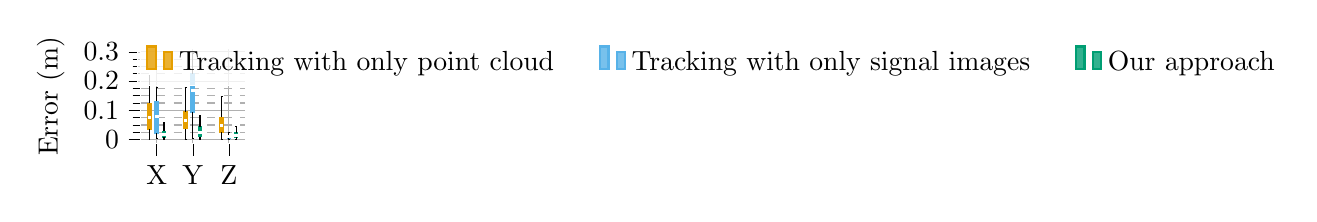
\begin{tikzpicture}

% \definecolor{color0}{rgb}{0.6,0,0.980392156862745}
% \definecolor{color1}{rgb}{0.968627450980392,0.00784313725490196,0.164705882352941}
% \definecolor{color2}{rgb}{0.0235294117647059,0.32156862745098,1}

\definecolor{color0}{rgb}{0.90, 0.62, 0.00}
\definecolor{color1}{rgb}{0.34, 0.70, 0.91}
\definecolor{color2}{rgb}{0.00, 0.62, 0.45}
\definecolor{color3}{rgb}{0.94, 0.89, 0.27}
\definecolor{color4}{rgb}{0.00, 0.45, 0.69}
\definecolor{color5}{rgb}{0.83, 0.37, 0.00}

\begin{axis}[
    width=\figurewidth,
    height=\figureheight,
    legend cell align={left},
    legend style={
      fill opacity=0.8,
      draw opacity=1,
      text opacity=1,
      at={(-0.03,1.10)},
      anchor=north west,
      draw=white,
      /tikz/every even column/.append style={column sep=0.5cm},
    },
    legend columns=3,
    axis line style={white},
    tick align=outside,
    tick pos=left,
    % title={Seq 1 },
    x grid style={white!69.0196078431373!black},
    xmin=0.5, xmax=6.3,
    xtick style={color=black},
    xtick={1.4,3.4,5.4},
    xticklabels={X,Y,Z},
    y grid style={white!69.0196078431373!black},
    ylabel={ Error (m)},
    ymin=-0.0147050240191961, ymax=0.31,
    ytick style={color=black},
    xmajorgrids,
    % xmajorticks=true,
    % xmin=-0.5, xmax=3.3125,
    xminorgrids,
    ymajorgrids,
    ymajorticks=true,
    minor y tick num = 3,
    minor y grid style={dashed},
    yminorgrids,
    yticklabel style={
            /pgf/number format/fixed,
            /pgf/number format/precision=5
    },
    scaled y ticks=false,
]

\draw[draw=color0,fill=color0, thick] (axis cs:0,0) rectangle (axis cs:0,0);
\addlegendimage{ybar, ybar legend, draw=color0,fill=color0,thick}
\addlegendentry{Tracking with only point cloud}

\draw[draw=color1,fill=color1, thick] (axis cs:0,0) rectangle (axis cs:0,0);
\addlegendimage{ybar, ybar legend, draw=color1,fill=color1,thick}
\addlegendentry{Tracking with only signal images}

\draw[draw=color2,fill=color2, thick] (axis cs:0,0) rectangle (axis cs:0,0);
\addlegendimage{ybar, ybar legend, draw=color2,fill=color2,thick}
\addlegendentry{Our approach}


\path [draw=color0, fill=color0]
(axis cs:0.9,0.0359016596706485)
--(axis cs:1.1,0.0359016596706485)
--(axis cs:1.1,0.123964853476531)
--(axis cs:0.9,0.123964853476531)
--(axis cs:0.9,0.0359016596706485)
--cycle;
\addplot [black, forget plot]
table {%
1 0.0359016596706485
1 0.000594158118181198
};
\addplot [black, forget plot]
table {%
1 0.123964853476531
1 0.219165955456631
};
\addplot [black, forget plot]
table {%
0.95 0.000594158118181198
1.05 0.000594158118181198
};
\addplot [black, forget plot]
table {%
0.95 0.219165955456631
1.05 0.219165955456631
};
\path [draw=color1, fill=color1]
(axis cs:1.3,0.0224564700129198)
--(axis cs:1.5,0.0224564700129198)
--(axis cs:1.5,0.131575909470591)
--(axis cs:1.3,0.131575909470591)
--(axis cs:1.3,0.0224564700129198)
--cycle;
\addplot [black, forget plot]
table {%
1.4 0.0224564700129198
1.4 0.00368735991092217
};
\addplot [black, forget plot]
table {%
1.4 0.131575909470591
1.4 0.177035822042366
};
\addplot [black, forget plot]
table {%
1.35 0.00368735991092217
1.45 0.00368735991092217
};
\addplot [black, forget plot]
table {%
1.35 0.177035822042366
1.45 0.177035822042366
};
\path [draw=color2, fill=color2]
(axis cs:1.7,0.00882856225400375)
--(axis cs:1.9,0.00882856225400375)
--(axis cs:1.9,0.0287960855190496)
--(axis cs:1.7,0.0287960855190496)
--(axis cs:1.7,0.00882856225400375)
--cycle;
\addplot [black, forget plot]
table {%
1.8 0.00882856225400375
1.8 0.000267686459507033
};
\addplot [black, forget plot]
table {%
1.8 0.0287960855190496
1.8 0.0584475453119366
};
\addplot [black, forget plot]
table {%
1.75 0.000267686459507033
1.85 0.000267686459507033
};
\addplot [black, forget plot]
table {%
1.75 0.0584475453119366
1.85 0.0584475453119366
};
\path [draw=color0, fill=color0]
(axis cs:2.9,0.0365788961205427)
--(axis cs:3.1,0.0365788961205427)
--(axis cs:3.1,0.0941762357336027)
--(axis cs:2.9,0.0941762357336027)
--(axis cs:2.9,0.0365788961205427)
--cycle;
\addplot [black, forget plot]
table {%
3 0.0365788961205427
3 0.000869162330838336
};
\addplot [black, forget plot]
table {%
3 0.0941762357336027
3 0.17826472756505
};
\addplot [black, forget plot]
table {%
2.95 0.000869162330838336
3.05 0.000869162330838336
};
\addplot [black, forget plot]
table {%
2.95 0.17826472756505
3.05 0.17826472756505
};
\path [draw=color1, fill=color1]
(axis cs:3.3,0.0936335797918026)
--(axis cs:3.5,0.0936335797918026)
--(axis cs:3.5,0.225292738533558)
--(axis cs:3.3,0.225292738533558)
--(axis cs:3.3,0.0936335797918026)
--cycle;
\addplot [black, forget plot]
table {%
3.4 0.0936335797918026
3.4 0.00413021189512097
};
\addplot [black, forget plot]
table {%
3.4 0.225292738533558
3.4 0.294725109117304
};
\addplot [black, forget plot]
table {%
3.35 0.00413021189512097
3.45 0.00413021189512097
};
\addplot [black, forget plot]
table {%
3.35 0.294725109117304
3.45 0.294725109117304
};
\path [draw=color2, fill=color2]
(axis cs:3.7,0.0105550124701859)
--(axis cs:3.9,0.0105550124701859)
--(axis cs:3.9,0.0439037283093395)
--(axis cs:3.7,0.0439037283093395)
--(axis cs:3.7,0.0105550124701859)
--cycle;
\addplot [black, forget plot]
table {%
3.8 0.0105550124701859
3.8 0.000138631389560828
};
\addplot [black, forget plot]
table {%
3.8 0.0439037283093395
3.8 0.0823405821542753
};
\addplot [black, forget plot]
table {%
3.75 0.000138631389560828
3.85 0.000138631389560828
};
\addplot [black, forget plot]
table {%
3.75 0.0823405821542753
3.85 0.0823405821542753
};
\path [draw=color0, fill=color0]
(axis cs:4.9,0.0255128619703696)
--(axis cs:5.1,0.0255128619703696)
--(axis cs:5.1,0.0756290965564553)
--(axis cs:4.9,0.0756290965564553)
--(axis cs:4.9,0.0255128619703696)
--cycle;
\addplot [black, forget plot]
table {%
5 0.0255128619703696
5 0.00148441613567574
};
\addplot [black, forget plot]
table {%
5 0.0756290965564553
5 0.148283764805501
};
\addplot [black, forget plot]
table {%
4.95 0.00148441613567574
5.05 0.00148441613567574
};
\addplot [black, forget plot]
table {%
4.95 0.148283764805501
5.05 0.148283764805501
};
\path [draw=color1, fill=color1]
(axis cs:5.3,0.00532853403802855)
--(axis cs:5.5,0.00532853403802855)
--(axis cs:5.5,0.0127842448158017)
--(axis cs:5.3,0.0127842448158017)
--(axis cs:5.3,0.00532853403802855)
--cycle;
\addplot [black, forget plot]
table {%
5.4 0.00532853403802855
5.4 0.00142377354419265
};
\addplot [black, forget plot]
table {%
5.4 0.0127842448158017
5.4 0.0237795656365393
};
\addplot [black, forget plot]
table {%
5.35 0.00142377354419265
5.45 0.00142377354419265
};
\addplot [black, forget plot]
table {%
5.35 0.0237795656365393
5.45 0.0237795656365393
};
\path [draw=color2, fill=color2]
(axis cs:5.7,0.00727972918056854)
--(axis cs:5.9,0.00727972918056854)
--(axis cs:5.9,0.0231674857426256)
--(axis cs:5.7,0.0231674857426256)
--(axis cs:5.7,0.00727972918056854)
--cycle;
\addplot [black, forget plot]
table {%
5.8 0.00727972918056854
5.8 2.9744225399142e-05
};
\addplot [black, forget plot]
table {%
5.8 0.0231674857426256
5.8 0.0459741988826368
};
\addplot [black, forget plot]
table {%
5.75 2.9744225399142e-05
5.85 2.9744225399142e-05
};
\addplot [black, forget plot]
table {%
5.75 0.0459741988826368
5.85 0.0459741988826368
};
\addplot [line width=1pt, white, forget plot]
table {%
0.9 0.0765784603353681
1.1 0.0765784603353681
};
\addplot [line width=1pt, white, forget plot]
table {%
1.3 0.0798680383669237
1.5 0.0798680383669237
};
\addplot [line width=1pt, white, forget plot]
table {%
1.7 0.0167689702781684
1.9 0.0167689702781684
};
\addplot [line width=1pt, white, forget plot]
table {%
2.9 0.0651368712573408
3.1 0.0651368712573408
};
\addplot [line width=1pt, white, forget plot]
table {%
3.3 0.167468870553379
3.5 0.167468870553379
};
\addplot [line width=1pt, white, forget plot]
table {%
3.7 0.0247040115872634
3.9 0.0247040115872634
};
\addplot [line width=1pt, white, forget plot]
table {%
4.9 0.0489386840818955
5.1 0.0489386840818955
};
\addplot [line width=1pt, white, forget plot]
table {%
5.3 0.00967427726703923
5.5 0.00967427726703923
};
\addplot [line width=1pt, white, forget plot]
table {%
5.7 0.0139552293806988
5.9 0.0139552293806988
};
\end{axis}

\end{tikzpicture}
}
        \caption{\scriptsize{Seq\,1}}
        \label{fig:err_seq1}
    \end{subfigure}
    \hfill
    \begin{subfigure}{.32\textwidth}
        \centering
        \setlength{\figurewidth}{\textwidth}
        \setlength{\figureheight}{1.03\textwidth}
        \scriptsize{% This file was created with tikzplotlib v0.9.14.
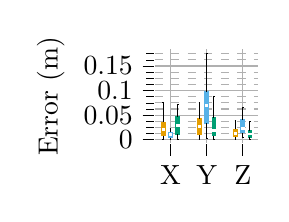
\begin{tikzpicture}

% \definecolor{color0}{rgb}{0.6,0,0.980392156862745}
% \definecolor{color1}{rgb}{0.968627450980392,0.00784313725490196,0.164705882352941}
% \definecolor{color2}{rgb}{0.0235294117647059,0.32156862745098,1}
\definecolor{color0}{rgb}{0.90, 0.62, 0.00}
\definecolor{color1}{rgb}{0.34, 0.70, 0.91}
\definecolor{color2}{rgb}{0.00, 0.62, 0.45}
\definecolor{color3}{rgb}{0.94, 0.89, 0.27}
\definecolor{color4}{rgb}{0.00, 0.45, 0.69}
\definecolor{color5}{rgb}{0.83, 0.37, 0.00}

\begin{axis}[
    width=\figurewidth,
    height=\figureheight,
    legend cell align={left},
    legend style={
      fill opacity=0.8,
      draw opacity=1,
      text opacity=1,
      at={(0.03,0.97)},
      anchor=north west,
      draw=white!80!black
    },
axis line style={white},
tick align=outside,
tick pos=left,
% title={Seq 2 },
x grid style={white!69.0196078431373!black},
xmin=0.5, xmax=6.3,
xtick style={color=black},
xtick={1.4,3.4,5.4},
xticklabels={X,Y,Z},
y grid style={white!69.0196078431373!black},
ylabel={ Error (m)},
ymin=-0.00876739680516033, ymax=0.184969536254822,
ytick style={color=black},
    xmajorgrids,
    % xmajorticks=true,
    % xmin=-0.5, xmax=3.3125,
    xminorgrids,
    ymajorgrids,
    ymajorticks=true,
    minor y tick num = 3,
    minor y grid style={dashed},
    yminorgrids,
    yticklabel style={
            /pgf/number format/fixed,
            /pgf/number format/precision=5
    },
    scaled y ticks=false,
]
\path [draw=color0, fill=color0]
(axis cs:0.9,0.00815245852515445)
--(axis cs:1.1,0.00815245852515445)
--(axis cs:1.1,0.0355660872611989)
--(axis cs:0.9,0.0355660872611989)
--(axis cs:0.9,0.00815245852515445)
--cycle;
\addplot [black, forget plot]
table {%
1 0.00815245852515445
1 0.000677464621831714
};
\addplot [black, forget plot]
table {%
1 0.0355660872611989
1 0.0760465676788473
};
\addplot [black, forget plot]
table {%
0.95 0.000677464621831714
1.05 0.000677464621831714
};
\addplot [black, forget plot]
table {%
0.95 0.0760465676788473
1.05 0.0760465676788473
};
\path [draw=color1, fill=color1]
(axis cs:1.3,0.00430830867868714)
--(axis cs:1.5,0.00430830867868714)
--(axis cs:1.5,0.0151839841291762)
--(axis cs:1.3,0.0151839841291762)
--(axis cs:1.3,0.00430830867868714)
--cycle;
\addplot [black, forget plot]
table {%
1.4 0.00430830867868714
1.4 0.0010557370823836
};
\addplot [black, forget plot]
table {%
1.4 0.0151839841291762
1.4 0.0231649600846127
};
\addplot [black, forget plot]
table {%
1.35 0.0010557370823836
1.45 0.0010557370823836
};
\addplot [black, forget plot]
table {%
1.35 0.0231649600846127
1.45 0.0231649600846127
};
\path [draw=color2, fill=color2]
(axis cs:1.7,0.0108070949987866)
--(axis cs:1.9,0.0108070949987866)
--(axis cs:1.9,0.0469455026016019)
--(axis cs:1.7,0.0469455026016019)
--(axis cs:1.7,0.0108070949987866)
--cycle;
\addplot [black, forget plot]
table {%
1.8 0.0108070949987866
1.8 3.88274248388498e-05
};
\addplot [black, forget plot]
table {%
1.8 0.0469455026016019
1.8 0.0722655397008891
};
\addplot [black, forget plot]
table {%
1.75 3.88274248388498e-05
1.85 3.88274248388498e-05
};
\addplot [black, forget plot]
table {%
1.75 0.0722655397008891
1.85 0.0722655397008891
};
\path [draw=color0, fill=color0]
(axis cs:2.9,0.00974226341835482)
--(axis cs:3.1,0.00974226341835482)
--(axis cs:3.1,0.0424458183453618)
--(axis cs:2.9,0.0424458183453618)
--(axis cs:2.9,0.00974226341835482)
--cycle;
\addplot [black, forget plot]
table {%
3 0.00974226341835482
3 0.0003648774884768
};
\addplot [black, forget plot]
table {%
3 0.0424458183453618
3 0.0759341926763533
};
\addplot [black, forget plot]
table {%
2.95 0.0003648774884768
3.05 0.0003648774884768
};
\addplot [black, forget plot]
table {%
2.95 0.0759341926763533
3.05 0.0759341926763533
};
\path [draw=color1, fill=color1]
(axis cs:3.3,0.0336190006785358)
--(axis cs:3.5,0.0336190006785358)
--(axis cs:3.5,0.097577699413025)
--(axis cs:3.3,0.097577699413025)
--(axis cs:3.3,0.0336190006785358)
--cycle;
\addplot [black, forget plot]
table {%
3.4 0.0336190006785358
3.4 0.0030644107688782
};
\addplot [black, forget plot]
table {%
3.4 0.097577699413025
3.4 0.176163312024822
};
\addplot [black, forget plot]
table {%
3.35 0.0030644107688782
3.45 0.0030644107688782
};
\addplot [black, forget plot]
table {%
3.35 0.176163312024822
3.45 0.176163312024822
};
\path [draw=color2, fill=color2]
(axis cs:3.7,0.00808186866347871)
--(axis cs:3.9,0.00808186866347871)
--(axis cs:3.9,0.0440748566983342)
--(axis cs:3.7,0.0440748566983342)
--(axis cs:3.7,0.00808186866347871)
--cycle;
\addplot [black, forget plot]
table {%
3.8 0.00808186866347871
3.8 0.0001008556550679
};
\addplot [black, forget plot]
table {%
3.8 0.0440748566983342
3.8 0.0881248202830607
};
\addplot [black, forget plot]
table {%
3.75 0.0001008556550679
3.85 0.0001008556550679
};
\addplot [black, forget plot]
table {%
3.75 0.0881248202830607
3.85 0.0881248202830607
};
\path [draw=color0, fill=color0]
(axis cs:4.9,0.00612243655419784)
--(axis cs:5.1,0.00612243655419784)
--(axis cs:5.1,0.0209237401912207)
--(axis cs:4.9,0.0209237401912207)
--(axis cs:4.9,0.00612243655419784)
--cycle;
\addplot [black, forget plot]
table {%
5 0.00612243655419784
5 0.000388261695153491
};
\addplot [black, forget plot]
table {%
5 0.0209237401912207
5 0.0392731995430584
};
\addplot [black, forget plot]
table {%
4.95 0.000388261695153491
5.05 0.000388261695153491
};
\addplot [black, forget plot]
table {%
4.95 0.0392731995430584
5.05 0.0392731995430584
};
\path [draw=color1, fill=color1]
(axis cs:5.3,0.0139338719068252)
--(axis cs:5.5,0.0139338719068252)
--(axis cs:5.5,0.040402023571507)
--(axis cs:5.3,0.040402023571507)
--(axis cs:5.3,0.0139338719068252)
--cycle;
\addplot [black, forget plot]
table {%
5.4 0.0139338719068252
5.4 0.00455167088083763
};
\addplot [black, forget plot]
table {%
5.4 0.040402023571507
5.4 0.065507495128893
};
\addplot [black, forget plot]
table {%
5.35 0.00455167088083763
5.45 0.00455167088083763
};
\addplot [black, forget plot]
table {%
5.35 0.065507495128893
5.45 0.065507495128893
};
\path [draw=color2, fill=color2]
(axis cs:5.7,0.004761184148176)
--(axis cs:5.9,0.004761184148176)
--(axis cs:5.9,0.0178303404227792)
--(axis cs:5.7,0.0178303404227792)
--(axis cs:5.7,0.004761184148176)
--cycle;
\addplot [black, forget plot]
table {%
5.8 0.004761184148176
5.8 0.000167742242199065
};
\addplot [black, forget plot]
table {%
5.8 0.0178303404227792
5.8 0.0364272724509153
};
\addplot [black, forget plot]
table {%
5.75 0.000167742242199065
5.85 0.000167742242199065
};
\addplot [black, forget plot]
table {%
5.75 0.0364272724509153
5.85 0.0364272724509153
};
\addplot [line width=1pt, white, forget plot]
table {%
0.9 0.0202748343545978
1.1 0.0202748343545978
};
\addplot [line width=1pt, white, forget plot]
table {%
1.3 0.00982938124535071
1.5 0.00982938124535071
};
\addplot [line width=1pt, white, forget plot]
table {%
1.7 0.029147362000046
1.9 0.029147362000046
};
\addplot [line width=1pt, white, forget plot]
table {%
2.9 0.0267552841689922
3.1 0.0267552841689922
};
\addplot [line width=1pt, white, forget plot]
table {%
3.3 0.0701316623582899
3.5 0.0701316623582899
};
\addplot [line width=1pt, white, forget plot]
table {%
3.7 0.0192756859440788
3.9 0.0192756859440788
};
\addplot [line width=1pt, white, forget plot]
table {%
4.9 0.0129318118170228
5.1 0.0129318118170228
};
\addplot [line width=1pt, white, forget plot]
table {%
5.3 0.0231806449570045
5.5 0.0231806449570045
};
\addplot [line width=1pt, white, forget plot]
table {%
5.7 0.0113959344884098
5.9 0.0113959344884098
};
\end{axis}

\end{tikzpicture}
}
        \caption{\scriptsize{Seq\,2}}
        \label{fig:err_seq2}     
    \end{subfigure}
    \hfill
    \begin{subfigure}{.32\textwidth}
        \centering
        \setlength{\figurewidth}{\textwidth}
        \setlength{\figureheight}{\textwidth}
        \scriptsize{% This file was created with tikzplotlib v0.9.14.
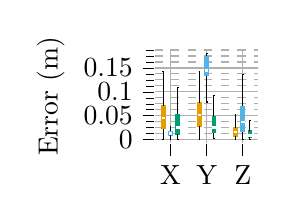
\begin{tikzpicture}

% \definecolor{color0}{rgb}{0.6,0,0.980392156862745}
% \definecolor{color1}{rgb}{0.968627450980392,0.00784313725490196,0.164705882352941}
% \definecolor{color2}{rgb}{0.0235294117647059,0.32156862745098,1}
\definecolor{color0}{rgb}{0.90, 0.62, 0.00}
\definecolor{color1}{rgb}{0.34, 0.70, 0.91}
\definecolor{color2}{rgb}{0.00, 0.62, 0.45}
\definecolor{color3}{rgb}{0.94, 0.89, 0.27}
\definecolor{color4}{rgb}{0.00, 0.45, 0.69}
\definecolor{color5}{rgb}{0.83, 0.37, 0.00}


\begin{axis}[
    width=\figurewidth,
    height=\figureheight,
    legend cell align={left},
    legend style={
      fill opacity=0.8,
      draw opacity=1,
      text opacity=1,
      at={(0.03,0.97)},
      anchor=north west,
      draw=white!80!black
    },
axis line style={white},
tick align=outside,
tick pos=left,
% title={Seq 3 },
x grid style={white!69.0196078431373!black},
xmin=0.5, xmax=6.3,
xtick style={color=black},
xtick={1.4,3.4,5.4},
xticklabels={X,Y,Z},
y grid style={white!69.0196078431373!black},
ylabel={ Error (m)},
ymin=-0.00897775582982006, ymax=0.189937849485646,
ytick style={color=black},
        xmajorgrids,
    % xmajorticks=true,
    % xmin=-0.5, xmax=3.3125,
    xminorgrids,
    ymajorgrids,
    ymajorticks=true,
    minor y tick num = 3,
    minor y grid style={dashed},
    yminorgrids,
    yticklabel style={
            /pgf/number format/fixed,
            /pgf/number format/precision=5
    },
    scaled y ticks=false,
]
\path [draw=color0, fill=color0]
(axis cs:0.9,0.0232780218577666)
--(axis cs:1.1,0.0232780218577666)
--(axis cs:1.1,0.0711417617143559)
--(axis cs:0.9,0.0711417617143559)
--(axis cs:0.9,0.0232780218577666)
--cycle;
\addplot [black, forget plot]
table {%
1 0.0232780218577666
1 0.000596100612618056
};
\addplot [black, forget plot]
table {%
1 0.0711417617143559
1 0.142771459094593
};
\addplot [black, forget plot]
table {%
0.95 0.000596100612618056
1.05 0.000596100612618056
};
\addplot [black, forget plot]
table {%
0.95 0.142771459094593
1.05 0.142771459094593
};
\path [draw=color1, fill=color1]
(axis cs:1.3,0.0088396449768362)
--(axis cs:1.5,0.0088396449768362)
--(axis cs:1.5,0.0177479663700559)
--(axis cs:1.3,0.0177479663700559)
--(axis cs:1.3,0.0088396449768362)
--cycle;
\addplot [black, forget plot]
table {%
1.4 0.0088396449768362
1.4 0.000359157874370908
};
\addplot [black, forget plot]
table {%
1.4 0.0177479663700559
1.4 0.0278344120708334
};
\addplot [black, forget plot]
table {%
1.35 0.000359157874370908
1.45 0.000359157874370908
};
\addplot [black, forget plot]
table {%
1.35 0.0278344120708334
1.45 0.0278344120708334
};
\path [draw=color2, fill=color2]
(axis cs:1.7,0.0114199810676545)
--(axis cs:1.9,0.0114199810676545)
--(axis cs:1.9,0.053081363686204)
--(axis cs:1.7,0.053081363686204)
--(axis cs:1.7,0.0114199810676545)
--cycle;
\addplot [black, forget plot]
table {%
1.8 0.0114199810676545
1.8 0.000901600574375827
};
\addplot [black, forget plot]
table {%
1.8 0.053081363686204
1.8 0.108638698498432
};
\addplot [black, forget plot]
table {%
1.75 0.000901600574375827
1.85 0.000901600574375827
};
\addplot [black, forget plot]
table {%
1.75 0.108638698498432
1.85 0.108638698498432
};
\path [draw=color0, fill=color0]
(axis cs:2.9,0.0279910207296199)
--(axis cs:3.1,0.0279910207296199)
--(axis cs:3.1,0.0771662866628215)
--(axis cs:2.9,0.0771662866628215)
--(axis cs:2.9,0.0279910207296199)
--cycle;
\addplot [black, forget plot]
table {%
3 0.0279910207296199
3 0.000493392369484091
};
\addplot [black, forget plot]
table {%
3 0.0771662866628215
3 0.14312320811591
};
\addplot [black, forget plot]
table {%
2.95 0.000493392369484091
3.05 0.000493392369484091
};
\addplot [black, forget plot]
table {%
2.95 0.14312320811591
3.05 0.14312320811591
};
\path [draw=color1, fill=color1]
(axis cs:3.3,0.133592629973776)
--(axis cs:3.5,0.133592629973776)
--(axis cs:3.5,0.1742756192671)
--(axis cs:3.3,0.1742756192671)
--(axis cs:3.3,0.133592629973776)
--cycle;
\addplot [black, forget plot]
table {%
3.4 0.133592629973776
3.4 0.0787552872431321
};
\addplot [black, forget plot]
table {%
3.4 0.1742756192671
3.4 0.180896231062216
};
\addplot [black, forget plot]
table {%
3.35 0.0787552872431321
3.45 0.0787552872431321
};
\addplot [black, forget plot]
table {%
3.35 0.180896231062216
3.45 0.180896231062216
};
\path [draw=color2, fill=color2]
(axis cs:3.7,0.0143334506366791)
--(axis cs:3.9,0.0143334506366791)
--(axis cs:3.9,0.0484907984263832)
--(axis cs:3.7,0.0484907984263832)
--(axis cs:3.7,0.0143334506366791)
--cycle;
\addplot [black, forget plot]
table {%
3.8 0.0143334506366791
3.8 0.00152332401541067
};
\addplot [black, forget plot]
table {%
3.8 0.0484907984263832
3.8 0.0919856255534661
};
\addplot [black, forget plot]
table {%
3.75 0.00152332401541067
3.85 0.00152332401541067
};
\addplot [black, forget plot]
table {%
3.75 0.0919856255534661
3.85 0.0919856255534661
};
\path [draw=color0, fill=color0]
(axis cs:4.9,0.00718570042061395)
--(axis cs:5.1,0.00718570042061395)
--(axis cs:5.1,0.02510844997279)
--(axis cs:4.9,0.02510844997279)
--(axis cs:4.9,0.00718570042061395)
--cycle;
\addplot [black, forget plot]
table {%
5 0.00718570042061395
5 0.000149403716627639
};
\addplot [black, forget plot]
table {%
5 0.02510844997279
5 0.0515712221274507
};
\addplot [black, forget plot]
table {%
4.95 0.000149403716627639
5.05 0.000149403716627639
};
\addplot [black, forget plot]
table {%
4.95 0.0515712221274507
5.05 0.0515712221274507
};
\path [draw=color1, fill=color1]
(axis cs:5.3,0.016524061983732)
--(axis cs:5.5,0.016524061983732)
--(axis cs:5.5,0.0702343830365995)
--(axis cs:5.3,0.0702343830365995)
--(axis cs:5.3,0.016524061983732)
--cycle;
\addplot [black, forget plot]
table {%
5.4 0.016524061983732
5.4 0.00088228305353566
};
\addplot [black, forget plot]
table {%
5.4 0.0702343830365995
5.4 0.136660089747208
};
\addplot [black, forget plot]
table {%
5.35 0.00088228305353566
5.45 0.00088228305353566
};
\addplot [black, forget plot]
table {%
5.35 0.136660089747208
5.45 0.136660089747208
};
\path [draw=color2, fill=color2]
(axis cs:5.7,0.00499251809664381)
--(axis cs:5.9,0.00499251809664381)
--(axis cs:5.9,0.0189492854816761)
--(axis cs:5.7,0.0189492854816761)
--(axis cs:5.7,0.00499251809664381)
--cycle;
\addplot [black, forget plot]
table {%
5.8 0.00499251809664381
5.8 6.38625936102422e-05
};
\addplot [black, forget plot]
table {%
5.8 0.0189492854816761
5.8 0.0394391370956968
};
\addplot [black, forget plot]
table {%
5.75 6.38625936102422e-05
5.85 6.38625936102422e-05
};
\addplot [black, forget plot]
table {%
5.75 0.0394391370956968
5.85 0.0394391370956968
};
\addplot [line width=1pt, white, forget plot]
table {%
0.9 0.0452829561791654
1.1 0.0452829561791654
};
\addplot [line width=1pt, white, forget plot]
table {%
1.3 0.0120809718295072
1.5 0.0120809718295072
};
\addplot [line width=1pt, white, forget plot]
table {%
1.7 0.0255258806510643
1.9 0.0255258806510643
};
\addplot [line width=1pt, white, forget plot]
table {%
2.9 0.0515489334434402
3.1 0.0515489334434402
};
\addplot [line width=1pt, white, forget plot]
table {%
3.3 0.14480473897281
3.5 0.14480473897281
};
\addplot [line width=1pt, white, forget plot]
table {%
3.7 0.025519191420708
3.9 0.025519191420708
};
\addplot [line width=1pt, white, forget plot]
table {%
4.9 0.0157743244749928
5.1 0.0157743244749928
};
\addplot [line width=1pt, white, forget plot]
table {%
5.3 0.0370830731462402
5.5 0.0370830731462402
};
\addplot [line width=1pt, white, forget plot]
table {%
5.7 0.00942297550400267
5.9 0.00942297550400267
};
\end{axis}

\end{tikzpicture}
}
        \caption{\scriptsize{Seq\,3}}
        \label{fig:err_seq3}     
    \end{subfigure}
    \caption{Absolute position error (APE) value of three data sequences.}
    \label{fig:ape_error} 
\end{figure*}


\begin{figure*}[t]
    \begin{subfigure}{.32\textwidth}
        \centering
        \setlength{\figurewidth}{\textwidth}
        \setlength{\figureheight}{\textwidth}
        \scriptsize{% This file was created with tikzplotlib v0.9.14.
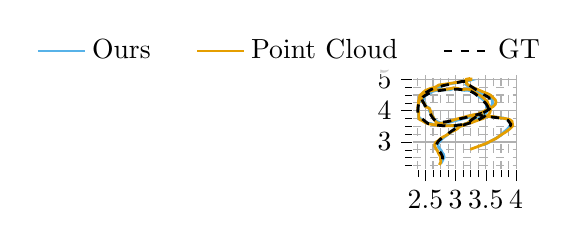
\begin{tikzpicture}

% \definecolor{color0}{rgb}{1,0.188235294117647,0.188235294117647}
\definecolor{color0}{rgb}{0.90, 0.62, 0.00}
\definecolor{color1}{rgb}{0.34, 0.70, 0.91}
\definecolor{color2}{rgb}{0.00, 0.62, 0.45}
\definecolor{color3}{rgb}{0.94, 0.89, 0.27}
\definecolor{color4}{rgb}{0.00, 0.45, 0.69}
\definecolor{color5}{rgb}{0.83, 0.37, 0.00}

\begin{axis}[
    width=\figurewidth,
    height=\figureheight,
legend cell align={left},
legend style={
  fill opacity=0.8,
  draw opacity=1,
  text opacity=1,
  at={(1.35,1.00)},
  anchor=south east,
  draw=white,
  /tikz/every even column/.append style={column sep=0.5cm},
},
legend columns=3,
axis line style= {white},
tick align=outside,
tick pos=left,
% title={XY plot},
xmajorgrids,
xmajorticks=true,
xminorgrids,
xminorgrids=true,
ymajorgrids,
ymajorticks=true,
yminorgrids,
yminorgrids=true,
    yticklabel style={
            /pgf/number format/fixed,
            /pgf/number format/precision=5
    },
    scaled y ticks=false,
        minor tick num = 3,
        minor grid style={dashed},
x grid style={white!69.0196078431373!black},
xmin=2.2937600641077, xmax=4.02480477083426,
xtick style={color=black},
y grid style={white!69.0196078431373!black},
ymin=2.12877276002231, ymax=5.16023554096054,
ytick style={color=black}
]
\addplot [line width=1pt, color1]
table {%
2.73259080042564 2.2954216427211
2.74343163560815 2.31777733333452
2.76226672899973 2.33763132237825
2.77197038543539 2.37099891932597
2.77941772327846 2.39915270681096
2.78829972509503 2.43237971210357
2.79987289003186 2.48228843678183
2.81119314984344 2.50723591521166
2.80290796777034 2.57016757457341
2.79863298401608 2.61110224606921
2.77857855552648 2.65472841443386
2.76879705733064 2.69645540690029
2.75941210404591 2.73302168382298
2.73673221300456 2.78460398196515
2.72048243208293 2.83162000452564
2.70981135271734 2.87356750945619
2.70740219155114 2.92110874032325
2.72064163397116 2.97777074365821
2.74227311431043 3.02254324868717
2.76767565170557 3.09168373521269
2.79776355687598 3.13921476015578
2.84619489817872 3.20421169494298
2.87781080242177 3.26403626073103
2.91866555366626 3.308839878853
2.95885920391216 3.35316934072594
2.99111507738432 3.39633428969372
3.01853055180776 3.43829247711476
3.04301459264569 3.47959461117091
3.07663927060839 3.50625344126635
3.11054872763804 3.52119343091084
3.12983829173943 3.55705093628962
3.17180958828291 3.58359333367066
3.22576927251157 3.61456898100191
3.28173252084285 3.66382379414986
3.33522348003846 3.70350267599603
3.38826456094178 3.73986772656383
3.42938132912533 3.79459211832735
3.47478516109619 3.8589167167674
3.49920348070984 3.92124063459251
3.51926711555732 3.99992257838136
3.53323378630256 4.04932519277265
3.5104876649043 4.12635767857896
3.50924029339517 4.18267360064715
3.49381577645071 4.26760867678425
3.46585263690297 4.33154077984819
3.42616129615141 4.40008314812554
3.39381158144173 4.44440381051309
3.35878389826143 4.50073852441353
3.31842252627628 4.54387388862518
3.28373377124474 4.57784565316582
3.26717255524395 4.61861403199193
3.20625048331003 4.65154330276112
3.14292769800767 4.64713122150596
3.10984578909261 4.65879743126192
3.03028290664255 4.70050728512957
2.98342308024528 4.71491058954871
2.90833750529192 4.66791998111957
2.81369016358825 4.66456338564272
2.68960518051834 4.6514615485341
2.61834317180246 4.61419404518564
2.59133359628131 4.57197420706711
2.53889867078703 4.53758470508788
2.49640102134837 4.46912709671841
2.43093337475764 4.42916135383894
2.41406072727463 4.34431157821041
2.38916320019083 4.25510880352394
2.38424727687088 4.19943957942588
2.3797065920442 4.10868519659685
2.3804940506239 4.03084815122655
2.38711249426717 3.96403028690104
2.38454997523936 3.87862436703802
2.38524487352131 3.81631763394191
2.4086064252633 3.75911789075354
2.44214202121798 3.71140899378346
2.47419208213707 3.65434881455194
2.52827375525438 3.60680009805964
2.59370041123844 3.58652056216466
2.64731952288101 3.55043822523879
2.73361202424747 3.53340288012352
2.81427216858312 3.52469800454746
2.90816328526587 3.52613146215501
2.96942244815454 3.50699401464921
3.04041606903737 3.54187917205913
3.08431936930925 3.53992240245697
3.13378486714116 3.55999978636447
3.15156481646775 3.58142860940515
3.19113576408744 3.59744380239372
3.20853207243552 3.61509018467778
3.22592080248474 3.64513837855198
3.24157625200172 3.67737153279367
3.26849122905683 3.70888977791336
3.29794225893743 3.76111119411413
3.34512934296052 3.81567450582051
3.3871017149695 3.87873492581653
3.44399595481758 3.94845073923546
3.50091762439694 4.00428374323119
3.55147346702835 4.07382113314224
3.58816732015563 4.13568268890664
3.61049923891057 4.22094809638009
3.60773687233267 4.28045051725409
3.60600726786476 4.35828816630771
3.55194239633667 4.4285547032453
3.51784149259861 4.47791919068106
3.43165381383551 4.55688852191186
3.36386457197198 4.62122417091992
3.29561769526148 4.68121848605205
3.24881431706591 4.73146398329164
3.20861244380214 4.78350441257105
3.16938767019224 4.83617557570634
3.18050056208889 4.88170283359478
3.16503509773993 4.93427000544225
3.208614253057 4.95618168663791
3.18412356131201 4.95904613541331
3.21190362926877 4.97156268814394
3.21027400805481 4.96111937046137
3.1700639722792 4.95360187519411
3.11517225580331 4.94110527615339
3.07335484285838 4.90874431955096
2.99570056124122 4.88445928190409
2.85846299112991 4.84402526283237
2.78757485262802 4.81363791051145
2.74221472731354 4.74639621909141
2.63435390947082 4.70270904061743
2.56660606991018 4.64008299046569
2.51794481030488 4.57376563144212
2.46911614289648 4.49753014236375
2.45058709697382 4.4323391667904
2.47135825381675 4.3752508721595
2.45283485458011 4.30350269834918
2.49496367430251 4.23780888271187
2.48904701255822 4.16120874459902
2.5646343025954 4.08395576213948
2.5687428966418 3.99330635987506
2.58730541323742 3.90717893497241
2.62251700243816 3.82396238528935
2.64333416476756 3.73051040945206
2.67948897550178 3.67380135412162
2.72166591565624 3.62732310185697
2.75270055594358 3.60816445200711
2.80677818151326 3.6098946166593
2.85133018420882 3.62974614417943
2.91066751505617 3.63564250016771
2.98482763034345 3.67777015015346
3.06730554673034 3.71591579123588
3.14460274091814 3.75898147583426
3.23213784635088 3.79552346889038
3.31024163079453 3.82217176546725
3.3512951091394 3.85307696350958
3.4017711046021 3.88682844445628
3.38549056476237 3.88813003946867
3.40526244113241 3.89499281734444
3.40346612365705 3.89927045065691
3.39371821855194 3.86211921707423
3.4019140630963 3.8675035459905
3.43280327400255 3.8550389843343
3.42039131920034 3.84582553031054
3.47478814252454 3.82192860675603
3.52481279222092 3.8188104365502
3.59465430557435 3.81326090765918
3.64292121266644 3.79713954466694
3.71732876891936 3.77813464376112
3.78228755694404 3.76760799931913
3.84326397997338 3.73444576200688
3.87591104971136 3.70009956408722
3.90045321168651 3.64725299707619
3.91996780654539 3.57459200766659
3.89384541236475 3.49507137704457
3.8532622045896 3.40462543050264
3.8009317601632 3.31878053771735
3.747730859615 3.21306244747252
3.66707106515983 3.11988218513941
3.5915272141181 3.03607055697764
3.52093959907854 2.95875103539358
3.45350962038186 2.90943214434925
};
\addlegendentry{Ours }
\addplot [line width=1pt, color0]
table {%
2.73138986085617 2.26656652279223
2.75360432320259 2.35714382130048
2.7508083515257 2.46912835587662
2.74550851348316 2.54904439484317
2.72250258307611 2.61610617873149
2.70890036336189 2.67091839597072
2.70048674867281 2.71293841304514
2.6621245905157 2.8289300166783
2.65258940451437 2.8774984141375
2.65388347721636 2.9297412196155
2.67367372667819 2.99582687673874
2.71430448120537 3.04398971125765
2.75246716597602 3.11821334733149
2.86294371432932 3.23500900778058
2.90622962533318 3.29710121648793
2.95056109235385 3.34523716767429
2.99364341688218 3.38133012793502
3.02859427991752 3.42218117361351
3.05303250126545 3.46468232077013
3.07371619488321 3.50232048035524
3.13888316455779 3.53138675226301
3.16026821946876 3.56050365837881
3.2011036391208 3.5866636872793
3.26194031975455 3.61679437274807
3.324686196072 3.66508438167831
3.39168199789358 3.71110243709038
3.45507064740115 3.74881729731915
3.54791406710348 3.87321212722207
3.56893738355065 3.94332451694098
3.57555290050113 4.02933308877975
3.58155283205009 4.09019776487595
3.54932629113885 4.16508434190537
3.53567629037423 4.22440220256894
3.51997284555271 4.30491172300629
3.433437696447 4.45110679138145
3.39377508547388 4.49818151091311
3.35114383424233 4.54490620065661
3.31313908978661 4.58474715181891
3.28820382358359 4.61732776598191
3.27425116100906 4.64513056496436
3.21557335445532 4.68209119320882
3.09517642619145 4.67689255581475
3.0237912725378 4.71121890184527
2.96730721438741 4.72908747193449
2.88654480121457 4.68988240652772
2.7825827012005 4.67061365107596
2.66926498137833 4.66318354414061
2.56055966975768 4.62011394913901
2.49794002158032 4.52897023159987
2.46771011458673 4.45192419369431
2.41016471761844 4.40100904910164
2.38746546621496 4.31615609623814
2.38373945569784 4.22276895453488
2.37568340169178 4.1513383273049
2.37438529736967 4.06132088987714
2.39164826922535 3.91240201883462
2.3902769834158 3.83365064700832
2.38948524431167 3.76827987219866
2.40738441948655 3.71381407610171
2.45310103488526 3.67536896327288
2.49340311007651 3.62523566406642
2.55163154853127 3.57816940186485
2.69675335918421 3.53342552792813
2.7828881224921 3.51982087848909
2.8781491291644 3.51785614866331
2.97401096266729 3.52830366103386
3.04490491628471 3.51297702842778
3.10674838697937 3.54607893560372
3.14268939458707 3.56705205771726
3.19304735985892 3.60401281076548
3.21979241206349 3.62928634441175
3.23261212494025 3.64446115856433
3.24157911978149 3.67286715948425
3.25282331608796 3.71002245775272
3.27531500357294 3.74868867147703
3.30946525165874 3.80102292687833
3.42385911017909 3.93236281040655
3.4925721935755 4.00647533265346
3.55868134397623 4.06658877149959
3.62211398508616 4.13244637976297
3.65590555658562 4.1961475001081
3.66762449416404 4.27739257805573
3.65635034189895 4.34797240131824
3.57450225759951 4.49815402389132
3.5158561928853 4.55318674767089
3.41539104845262 4.63109920128498
3.33620951102076 4.70003778680557
3.25981144745224 4.76173411000382
3.21774691837508 4.80983644276065
3.18190880196593 4.85795678179988
3.17415752571927 4.94957756098052
3.17693561005654 5.00200282074395
3.22823553566057 5.02244177819062
3.23357894433589 5.01361867542625
3.25220577008086 5.01083580216477
3.2515280013004 4.99080038985157
3.20585824063552 4.97426244268442
3.06770239653192 4.92098387821703
2.97668730023826 4.89068955830255
2.84576909514051 4.85105684806315
2.72324522445048 4.81949275852938
2.66511587162346 4.75215494766644
2.56737987444208 4.7000965492915
2.49471329396189 4.6370482848981
2.4093239167304 4.48600491487912
2.39956970376416 4.4143954307876
2.4376903406125 4.35508778149186
2.44608059076592 4.28856147136882
2.49113634814668 4.21924292669192
2.49765126578515 4.14232480811796
2.57138202453032 4.05807420954335
2.60142040165522 3.87004989365037
2.63148326539495 3.78420504498652
2.65489646110252 3.69286429381683
2.67590307732644 3.63283440896259
2.71555056669599 3.60052766507381
2.75553028398983 3.59385470673663
2.80934333571462 3.61573660602321
2.92733741621492 3.67854550142618
3.00795400936487 3.72883539212453
3.113924435822 3.78066445016795
3.20209421874616 3.82685738124627
3.29513009591462 3.86869615050429
3.37406738163484 3.89120954533684
3.41678144100867 3.91382799082125
3.42748138373125 3.9365317018496
3.41629296783595 3.93210645408647
3.39991136029194 3.93231502623131
3.38655207560852 3.89157036167549
3.38100526590359 3.87612959104443
3.41160372311744 3.86039258272765
3.42411932536854 3.84920205010396
3.46911867279182 3.82223804415004
3.62774585499471 3.81118702895529
3.68700583597362 3.78918835850452
3.76279959859637 3.76273740012428
3.83677982126538 3.74379930250183
3.89950867841041 3.71244778006224
3.93350333458381 3.66098633321622
3.94612092052851 3.51781356500873
3.90038448028181 3.42482929034603
3.83280522309102 3.32435618429358
3.75225049030137 3.22850809599341
3.67462506650057 3.12001769870334
3.57868141193329 3.02508054511676
3.48884590654207 2.9409249519996
3.33868769525814 2.83436894351627
3.27961156151381 2.79343853460443
3.24219519876619 2.76691028471854
};
\addlegendentry{Point Cloud}
% \addplot [line width=1pt, green!50!black]
% table {%
% 2.79194092027163 2.35892892452518
% 2.79407119406988 2.42978630582589
% 2.79527527534208 2.48453329989567
% 2.79418461279521 2.53544276599431
% 2.7992917117979 2.60163917930246
% 2.81102871558341 2.63961579753378
% 2.79760860772589 2.70738974953776
% 2.78645569767935 2.75855673276656
% 2.75987040227934 2.8035775783111
% 2.74492820427677 2.84376380208128
% 2.73700166567946 2.8750528381069
% 2.71236227704775 2.92158934911775
% 2.68765841775157 2.97520109740467
% 2.67290493528827 3.02040086164092
% 2.66640708423765 3.06965739993503
% 2.67907644603627 3.13503458401981
% 2.71122620765581 3.1852448045617
% 2.73898108045827 3.26139294599305
% 2.78053817349636 3.31810043051243
% 2.83576546128013 3.38685611116533
% 2.86746986064176 3.45422213542551
% 2.90443960573929 3.50698442114095
% };
% \addlegendentry{Image}
\addplot [line width=1pt, black, dashed]
table {%
2.78004336357117 2.44961881637573
2.78473997116089 2.49184632301331
2.78169870376587 2.53642201423645
2.77279257774353 2.5811128616333
2.7611358165741 2.62548923492432
2.74732780456543 2.66858124732971
2.73093748092651 2.71244502067566
2.69390487670898 2.80324053764343
2.68285369873047 2.84974360466003
2.68129086494446 2.89853239059448
2.68994092941284 2.95167922973633
2.7073175907135 3.00733399391174
2.73254680633545 3.06419110298157
2.80578780174255 3.17853021621704
2.84787058830261 3.23518180847168
2.89023494720459 3.28984522819519
2.9271776676178 3.34109807014465
2.96092367172241 3.38540554046631
2.99176788330078 3.42358613014221
3.02260088920593 3.4562566280365
3.08351445198059 3.50875163078308
3.11538076400757 3.53420877456665
3.15450525283813 3.55867266654968
3.20232772827148 3.58785653114319
3.25803208351135 3.6181046962738
3.3161768913269 3.65492224693298
3.37219643592834 3.70083785057068
3.47152757644653 3.80997467041016
3.50878357887268 3.87289643287659
3.53404450416565 3.93877172470093
3.54474639892578 4.00425100326538
3.54177737236023 4.07564973831177
3.5278651714325 4.14390993118286
3.50693893432617 4.21157598495483
3.44325828552246 4.34743690490723
3.41175317764282 4.3992977142334
3.38133764266968 4.44696283340454
3.34080910682678 4.50991916656494
3.31128025054932 4.55272197723389
3.27819752693176 4.59152603149414
3.23718738555908 4.62049102783203
3.13333964347839 4.66143894195557
3.0713849067688 4.67684459686279
3.00010514259338 4.68613862991333
2.93614459037781 4.68156385421753
2.84673571586609 4.67292547225952
2.7660768032074 4.65167999267578
2.68826532363892 4.62711381912231
2.56908178329468 4.56195640563965
2.4967725276947 4.48921155929565
2.45544767379761 4.42907476425171
2.42531800270081 4.364417552948
2.39972305297852 4.28832912445068
2.38822770118713 4.21258687973022
2.38112616539001 4.13534498214722
2.37244391441345 3.9815731048584
2.37436366081238 3.91040086746216
2.38197445869446 3.84459114074707
2.38410639762878 3.83271741867065
2.38410639762878 3.83271741867065
2.54188394546509 3.59143424034119
2.54188394546509 3.59143424034119
2.63489747047424 3.55322051048279
2.71523118019104 3.53378105163574
2.79587984085083 3.52052617073059
2.87371587753296 3.51484632492065
2.94537568092346 3.51649236679077
3.00989937782288 3.52600789070129
3.02894711494446 3.53686928749084
3.1410870552063 3.56351637840271
3.16888523101807 3.57629799842834
3.19266724586487 3.59665036201477
3.21331095695496 3.62381148338318
3.23522543907166 3.65565609931946
3.25612902641296 3.696049451828
3.28694272041321 3.73732781410217
3.37403917312622 3.84776592254639
3.43747353553772 3.91309595108032
3.46730494499207 3.94392347335815
3.54685282707214 4.03354120254517
3.56150364875793 4.05302429199219
3.56150364875793 4.05302429199219
3.55420994758606 4.41191577911377
3.55420994758606 4.41191577911377
3.52897119522095 4.44498062133789
3.46123027801514 4.51591968536377
3.44793391227722 4.52946996688843
3.44793391227722 4.52946996688843
3.20479941368103 4.8422794342041
3.20479941368103 4.8422794342041
3.20333743095398 4.84621095657349
3.19610905647278 4.88337802886963
3.20433259010315 4.92765474319458
3.20877623558044 4.93645238876343
3.20877623558044 4.93645238876343
3.10875654220581 4.93231248855591
3.10875654220581 4.93231248855591
3.09200954437256 4.92480373382568
3.0337131023407 4.9000825881958
2.81984186172485 4.80996656417847
2.81984186172485 4.80996656417847
2.74672770500183 4.77510261535645
2.66049242019653 4.72225284576416
2.59113669395447 4.67178773880005
2.47602367401123 4.53933477401733
2.44892525672913 4.4741735458374
2.44124889373779 4.4066367149353
2.44737863540649 4.33526086807251
2.46477293968201 4.2646312713623
2.48559141159058 4.19270467758179
2.5109715461731 4.11613798141479
2.56022667884827 3.95782518386841
2.59123277664185 3.86118698120117
2.61795139312744 3.78020834922791
2.64434695243835 3.71509742736816
2.67542433738708 3.66681861877441
2.7141900062561 3.63695573806763
2.75917601585388 3.62501287460327
2.87690043449402 3.65587210655212
2.94824028015137 3.68864607810974
3.02909922599792 3.72396874427795
3.1125910282135 3.75977635383606
3.19374990463257 3.79366683959961
3.25704741477966 3.82296109199524
3.32147431373596 3.85447812080383
3.3886239528656 3.89113712310791
3.3969361782074 3.89532256126404
3.39630007743835 3.89313435554504
3.3953697681427 3.88669848442078
3.39798903465271 3.8734872341156
3.4073429107666 3.85793447494507
3.42936635017395 3.84170961380005
3.45953583717346 3.82747554779053
3.5581591129303 3.80352425575256
3.62155294418335 3.7911856174469
3.69111347198486 3.77538084983826
3.76070165634155 3.75537896156311
3.82333898544312 3.72709131240845
3.86648988723755 3.69070506095886
3.91346454620361 3.56822967529297
3.89978837966919 3.49198365211487
3.86199855804443 3.40586566925049
3.81219482421875 3.32272267341614
3.81219482421875 3.32272267341614
3.81219482421875 3.32272267341614
3.81219482421875 3.32272267341614
3.81219482421875 3.32272267341614
3.81219482421875 3.32272267341614
3.81219482421875 3.32272267341614
};
\addlegendentry{GT}
\end{axis}

\end{tikzpicture}
}
        \caption{\scriptsize{XY trajectory plot}}
        \label{fig:xy_plot}
    \end{subfigure}
    \hfill
    \begin{subfigure}{.32\textwidth}
        \centering
        \setlength{\figurewidth}{\textwidth}
        \setlength{\figureheight}{\textwidth}
        \scriptsize{% This file was created with tikzplotlib v0.9.14.
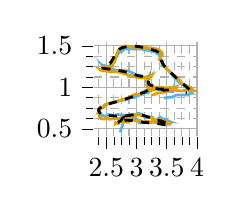
\begin{tikzpicture}

% \definecolor{color0}{rgb}{1,0.188235294117647,0.188235294117647}
\definecolor{color0}{rgb}{0.90, 0.62, 0.00}
\definecolor{color1}{rgb}{0.34, 0.70, 0.91}
\definecolor{color2}{rgb}{0.00, 0.62, 0.45}
\definecolor{color3}{rgb}{0.94, 0.89, 0.27}
\definecolor{color4}{rgb}{0.00, 0.45, 0.69}
\definecolor{color5}{rgb}{0.83, 0.37, 0.00}

\begin{axis}[
    width=\figurewidth,
    height=\figureheight,
legend cell align={left},
legend style={
  fill opacity=0.8,
  draw opacity=1,
  text opacity=1,
  at={(0.97,0.03)},
  anchor=south east,
  draw=white!80!black
},
axis line style= {white},
tick align=outside,
tick pos=left,
% title={XY plot},
xmajorgrids,
xmajorticks=true,
xminorgrids,
xminorgrids=true,
ymajorgrids,
ymajorticks=true,
yminorgrids,
yminorgrids=true,
    yticklabel style={
            /pgf/number format/fixed,
            /pgf/number format/precision=5
    },
    scaled y ticks=false,
            minor tick num = 3,
        minor grid style={dashed},
x grid style={white!69.0196078431373!black},
xmin=2.2937600641077, xmax=4.02480477083426,
xtick style={color=black},
y grid style={white!69.0196078431373!black},
ymin=0.404950771684837, ymax=1.54912152663555,
ytick style={color=black}
]
\addplot [line width=1pt, color1]
table {%
2.73259080042564 0.456958533273505
2.74343163560815 0.49487950715315
2.76226672899973 0.529290846679961
2.77197038543539 0.558159603164172
2.77941772327846 0.581603031021609
2.78829972509503 0.611786834903712
2.79987289003186 0.619828840130322
2.81119314984344 0.618996725006725
2.80290796777034 0.628498933188615
2.79863298401608 0.618617386776924
2.77857855552648 0.614607834975727
2.76879705733064 0.595761471537237
2.75941210404591 0.587547656728352
2.73673221300456 0.590958649413665
2.72048243208293 0.591881436489796
2.70981135271734 0.587976674053637
2.70740219155114 0.602002696201986
2.72064163397116 0.60076945794349
2.74227311431043 0.599485724584289
2.76767565170557 0.606668274298737
2.79776355687598 0.601798888398763
2.84619489817872 0.601803934405946
2.87781080242177 0.624994661038883
2.91866555366626 0.618054264314445
2.95885920391216 0.633184133508421
2.99111507738432 0.621581680741958
3.01853055180776 0.608653774943656
3.04301459264569 0.575099462250055
3.07663927060839 0.572568446543079
3.11054872763804 0.572684579097422
3.12983829173943 0.582454008587114
3.17180958828291 0.572830630436128
3.22576927251157 0.57180452551432
3.28173252084285 0.591655611703931
3.33522348003846 0.601012115979793
3.38826456094178 0.597981792655272
3.42938132912533 0.583684884156747
3.47478516109619 0.588966843957799
3.49920348070984 0.59836364931814
3.51926711555732 0.597582087944079
3.53323378630256 0.593434769797821
3.5104876649043 0.595421832362148
3.50924029339517 0.587168678823642
3.49381577645071 0.61323269863585
3.46585263690297 0.619632582003686
3.42616129615141 0.616422580950774
3.39381158144173 0.642036095741194
3.35878389826143 0.627756915178666
3.31842252627628 0.600471148141839
3.28373377124474 0.616949772980762
3.26717255524395 0.638238638834733
3.20625048331003 0.644806702267674
3.14292769800767 0.63367921735363
3.10984578909261 0.669634341593406
3.03028290664255 0.689264916110825
2.98342308024528 0.670265382912131
2.90833750529192 0.673432023045431
2.81369016358825 0.663546258504555
2.68960518051834 0.673433980979231
2.61834317180246 0.658970398827948
2.59133359628131 0.666703837043153
2.53889867078703 0.671934417412527
2.49640102134837 0.653844414067499
2.43093337475764 0.65968524912859
2.41406072727463 0.685358084016413
2.38916320019083 0.69307586205989
2.38424727687088 0.701937000010989
2.3797065920442 0.720095622449483
2.3804940506239 0.724435974931953
2.38711249426717 0.731778433289824
2.38454997523936 0.741309372872078
2.38524487352131 0.734836655091209
2.4086064252633 0.761445802916635
2.44214202121798 0.759670298112906
2.47419208213707 0.789383693822738
2.52827375525438 0.803059543989636
2.59370041123844 0.813322396882952
2.64731952288101 0.824897819019936
2.73361202424747 0.840585453207842
2.81427216858312 0.849309565324545
2.90816328526587 0.879255694390182
2.96942244815454 0.87885509882795
3.04041606903737 0.904607260521757
3.08431936930925 0.911776331357928
3.13378486714116 0.926187070720048
3.15156481646775 0.934689504021621
3.19113576408744 0.933546064274718
3.20853207243552 0.954467023878263
3.22592080248474 0.966678058414332
3.24157625200172 0.956835685894477
3.26849122905683 0.973457766206282
3.29794225893743 0.976457955699481
3.34512934296052 0.978880187295118
3.3871017149695 0.978734109121055
3.44399595481758 0.96995812975022
3.50091762439694 0.97968247290656
3.55147346702835 0.964835905435578
3.58816732015563 0.963451033157929
3.61049923891057 0.995157931634678
3.60773687233267 0.972477292621147
3.60600726786476 0.951715788645927
3.55194239633667 0.95058415575198
3.51784149259861 0.960707664166411
3.43165381383551 0.984419651304546
3.36386457197198 0.971751831612376
3.29561769526148 0.985980195289496
3.24881431706591 1.00240644796764
3.20861244380214 1.01293429952561
3.16938767019224 1.02839853580769
3.18050056208889 1.05042831139707
3.16503509773993 1.08165869271809
3.208614253057 1.1164418127072
3.18412356131201 1.10544999991501
3.21190362926877 1.14284870029486
3.21027400805481 1.13248620425793
3.1700639722792 1.12856981396099
3.11517225580331 1.12136826430779
3.07335484285838 1.13975526380678
2.99570056124122 1.15118368116767
2.85846299112991 1.19951970322011
2.78757485262802 1.20221132249522
2.74221472731354 1.20186365755875
2.63435390947082 1.21033719632458
2.56660606991018 1.21925373592581
2.51794481030488 1.22002153597137
2.46911614289648 1.23972725018781
2.45058709697382 1.25168273938092
2.47135825381675 1.23057699533913
2.45283485458011 1.25793334385766
2.49496367430251 1.23861195945078
2.48904701255822 1.25862519873877
2.5646343025954 1.24417509580164
2.5687428966418 1.26722145795548
2.58730541323742 1.28285985998207
2.62251700243816 1.29433042920734
2.64333416476756 1.33602361791541
2.67948897550178 1.38722348527647
2.72166591565624 1.42740486735385
2.75270055594358 1.43096683264484
2.80677818151326 1.46420167865521
2.85133018420882 1.4606499087354
2.91066751505617 1.4628090494307
2.98482763034345 1.45993833472835
3.06730554673034 1.46263587920374
3.14460274091814 1.44949469574389
3.23213784635088 1.44062697468932
3.31024163079453 1.4270307741753
3.3512951091394 1.40036671651812
3.4017711046021 1.39766894649338
3.38549056476237 1.37806342977231
3.40526244113241 1.37318389131059
3.40346612365705 1.36299155725777
3.39371821855194 1.33984612380685
3.4019140630963 1.32903653727561
3.43280327400255 1.31918825508543
3.42039131920034 1.266029771924
3.47478814252454 1.23864452174203
3.52481279222092 1.20708994254779
3.59465430557435 1.14070726337675
3.64292121266644 1.11078098661924
3.71732876891936 1.04934668163039
3.78228755694404 1.02317563752568
3.84326397997338 0.97866913059187
3.87591104971136 0.953033900190684
3.90045321168651 0.941730769001205
3.91996780654539 0.928809906030269
3.89384541236475 0.928975172026874
3.8532622045896 0.908870429954832
3.8009317601632 0.906522072719271
3.747730859615 0.906822278537671
3.66707106515983 0.907357408886252
3.5915272141181 0.883460231704356
3.52093959907854 0.878559911280428
3.45350962038186 0.871585647476596
};
% \addlegendentry{Ours}
\addplot [line width=1pt, color0]
table {%
2.73138986085617 0.657010612239058
2.75360432320259 0.645698437987604
2.7508083515257 0.646742571562861
2.74550851348316 0.62647268601071
2.72250258307611 0.615033248815969
2.70890036336189 0.587527391166454
2.70048674867281 0.566557237876796
2.6621245905157 0.56724183290176
2.65258940451437 0.562835575197254
2.65388347721636 0.574767195104584
2.67367372667819 0.569375858413319
2.71430448120537 0.580960908636404
2.75246716597602 0.589230026100572
2.86294371432932 0.578972956710099
2.90622962533318 0.602869530796653
2.95056109235385 0.610498545305097
2.99364341688218 0.592091640957174
3.02859427991752 0.596601918924841
3.05303250126545 0.605446191691559
3.07371619488321 0.59331040534939
3.13888316455779 0.578954124385501
3.16026821946876 0.593471293840019
3.2011036391208 0.587441829084113
3.26194031975455 0.585436550167668
3.324686196072 0.574030825320271
3.39168199789358 0.583491131606597
3.45507064740115 0.590701699692942
3.54791406710348 0.565351407396609
3.56893738355065 0.569375888805397
3.57555290050113 0.573217204811524
3.58155283205009 0.578697321920415
3.54932629113885 0.558774371932346
3.53567629037423 0.570017814051165
3.51997284555271 0.580211876341465
3.433437696447 0.601787538331989
3.39377508547388 0.616557406612546
3.35114383424233 0.606157718175345
3.31313908978661 0.603748215910125
3.28820382358359 0.612260202930852
3.27425116100906 0.623836672256871
3.21557335445532 0.639473359682488
3.09517642619145 0.656413354814575
3.0237912725378 0.671493474375941
2.96730721438741 0.660581288371215
2.88654480121457 0.651813349136982
2.7825827012005 0.619723430507855
2.66926498137833 0.625654022015665
2.56055966975768 0.616804803660629
2.49794002158032 0.633532465778361
2.46771011458673 0.618005370455619
2.41016471761844 0.622471582166816
2.38746546621496 0.648487353780215
2.38373945569784 0.682968405146507
2.37568340169178 0.685387413787086
2.37438529736967 0.701568477070616
2.39164826922535 0.729654784320017
2.3902769834158 0.736487016563697
2.38948524431167 0.735191718975739
2.40738441948655 0.747989026078135
2.45310103488526 0.757754302568014
2.49340311007651 0.787481070169994
2.55163154853127 0.808336627680076
2.69675335918421 0.837018512573694
2.7828881224921 0.857900350992185
2.8781491291644 0.87983859016243
2.97401096266729 0.914689697777957
3.04490491628471 0.91779790983678
3.10674838697937 0.942201302549024
3.14268939458707 0.96160500839244
3.19304735985892 0.968176824179276
3.21979241206349 0.977424816005104
3.23261212494025 0.98854923733403
3.24157911978149 0.997481256467301
3.25282331608796 0.999000764258679
3.27531500357294 1.00551834148556
3.30946525165874 1.00210401950882
3.42385911017909 1.00202748043467
3.4925721935755 0.991707550655818
3.55868134397623 0.999853118029554
3.62211398508616 0.987300409123901
3.65590555658562 0.980690779878946
3.66762449416404 1.00865384311342
3.65635034189895 1.00505626919742
3.57450225759951 0.964686392024289
3.5158561928853 0.975173104382569
3.41539104845262 0.992214323705194
3.33620951102076 0.977635694403429
3.25981144745224 0.970582182546276
3.21774691837508 0.98772491904037
3.18190880196593 1.00187251057426
3.17415752571927 1.04332747828965
3.17693561005654 1.08104896882526
3.22823553566057 1.13409488077488
3.23357894433589 1.12385764666774
3.25220577008086 1.14058092021073
3.2515280013004 1.13862285041618
3.20585824063552 1.12637073288414
3.06770239653192 1.11237674535651
2.97668730023826 1.12632378485632
2.84576909514051 1.15338153706751
2.72324522445048 1.1802201492966
2.66511587162346 1.189201715826
2.56737987444208 1.18631715643634
2.49471329396189 1.19710683876199
2.4093239167304 1.20630857760943
2.39956970376416 1.21285429981377
2.4376903406125 1.202070126601
2.44608059076592 1.23690657263644
2.49113634814668 1.22873410169901
2.49765126578515 1.24007702537664
2.57138202453032 1.22883324088849
2.60142040165522 1.27584502213182
2.63148326539495 1.30200693519575
2.65489646110252 1.35019264639585
2.67590307732644 1.41278413765946
2.71555056669599 1.46554881335009
2.75553028398983 1.48216535325547
2.80934333571462 1.49711376504688
2.92733741621492 1.48416807027805
3.00795400936487 1.48239981199108
3.113924435822 1.48464560222221
3.20209421874616 1.47546689225864
3.29513009591462 1.46906545974477
3.37406738163484 1.45005143552191
3.41678144100867 1.42274324602061
3.42748138373125 1.39132730307169
3.41629296783595 1.3824463086832
3.39991136029194 1.36938887207413
3.38655207560852 1.34900145876894
3.38100526590359 1.33633294363003
3.41160372311744 1.32677290340083
3.42411932536854 1.29090759232864
3.46911867279182 1.24151728469815
3.62774585499471 1.14207346885956
3.68700583597362 1.10617092039616
3.76279959859637 1.04095998209618
3.83677982126538 1.01456959616795
3.89950867841041 0.997756247245787
3.93350333458381 0.968176820352702
3.94612092052851 0.962598085536201
3.90038448028181 0.967805219897478
3.83280522309102 0.969189952480515
3.75225049030137 0.956281648576645
3.67462506650057 0.96179460005697
3.57868141193329 0.973224968241479
3.48884590654207 0.945283145524123
3.33868769525814 0.928901271267334
3.27961156151381 0.909942415671177
3.24219519876619 0.906760277506214
};
% \addlegendentry{Point Cloud}
% \addplot [line width=1pt, green!50!black]
% table {%
% 2.79194092027163 0.675682647712128
% 2.79407119406988 0.703220041949035
% 2.79527527534208 0.711795270023535
% 2.79418461279521 0.726723723913668
% 2.7992917117979 0.727191847951841
% 2.81102871558341 0.713931684485897
% 2.79760860772589 0.702141990464947
% 2.78645569767935 0.677849089690324
% 2.75987040227934 0.655033487836737
% 2.74492820427677 0.622901863605389
% 2.73700166567946 0.58679370241161
% 2.71236227704775 0.564860313864813
% 2.68765841775157 0.564271594380181
% 2.67290493528827 0.559782760866558
% 2.66640708423765 0.565083992103844
% 2.67907644603627 0.555989880189345
% 2.71122620765581 0.563908618052208
% 2.73898108045827 0.569398247074381
% 2.78053817349636 0.560509803672526
% 2.83576546128013 0.56673625834506
% 2.86746986064176 0.591594042425316
% 2.90443960573929 0.60198713859095
% };
% \addlegendentry{Image}
\addplot [line width=1pt, black, dashed]
table {%
2.78004336357117 0.632818698883057
2.78473997116089 0.638318061828613
2.78169870376587 0.637591958045959
2.77279257774353 0.63290148973465
2.7611358165741 0.621461033821106
2.74732780456543 0.60774290561676
2.73093748092651 0.594337582588196
2.69390487670898 0.576365888118744
2.68285369873047 0.575522303581238
2.68129086494446 0.578539431095123
2.68994092941284 0.580935955047607
2.7073175907135 0.584364891052246
2.73254680633545 0.5893794298172
2.80578780174255 0.601789712905884
2.84787058830261 0.6033616065979
2.89023494720459 0.602049291133881
2.9271776676178 0.600774049758911
2.96092367172241 0.598361253738403
2.99176788330078 0.595715701580048
3.02260088920593 0.592634737491608
3.08351445198059 0.582817792892456
3.11538076400757 0.578564763069153
3.15450525283813 0.578361749649048
3.20232772827148 0.575249850749969
3.25803208351135 0.574694573879242
3.3161768913269 0.57064300775528
3.37219643592834 0.561338245868683
3.47152757644653 0.548518240451813
3.50878357887268 0.548225939273834
3.53404450416565 0.550397217273712
3.54474639892578 0.557612478733063
3.54177737236023 0.559260010719299
3.5278651714325 0.562194406986237
3.50693893432617 0.567442297935486
3.44325828552246 0.58589380979538
3.41175317764282 0.595011711120605
3.38133764266968 0.600455462932587
3.34080910682678 0.605159401893616
3.31128025054932 0.609150171279907
3.27819752693176 0.617089152336121
3.23718738555908 0.632509291172028
3.13333964347839 0.658334314823151
3.0713849067688 0.666970789432526
3.00010514259338 0.668299496173859
2.93614459037781 0.668152689933777
2.84673571586609 0.659588932991028
2.7660768032074 0.65624737739563
2.68826532363892 0.652865469455719
2.56908178329468 0.658845484256744
2.4967725276947 0.667507708072662
2.45544767379761 0.673418462276459
2.42531800270081 0.681628286838531
2.39972305297852 0.689211785793304
2.38822770118713 0.697850942611694
2.38112616539001 0.707625448703766
2.37244391441345 0.725314617156982
2.37436366081238 0.734794139862061
2.38197445869446 0.744607985019684
2.38410639762878 0.745479464530945
2.38410639762878 0.745479464530945
2.54188394546509 0.801227807998657
2.54188394546509 0.801227807998657
2.63489747047424 0.819602787494659
2.71523118019104 0.835769176483154
2.79587984085083 0.853483378887177
2.87371587753296 0.872008979320526
2.94537568092346 0.889821469783783
3.00989937782288 0.904130518436432
3.02894711494446 0.918487727642059
3.1410870552063 0.944109201431274
3.16888523101807 0.957380533218384
3.19266724586487 0.966566443443298
3.21331095695496 0.975494146347046
3.23522543907166 0.986978530883789
3.25612902641296 0.986358344554901
3.28694272041321 0.991490304470062
3.37403917312622 0.979946970939636
3.43747353553772 0.979255378246307
3.46730494499207 0.978964030742645
3.54685282707214 0.97417813539505
3.56150364875793 0.973176598548889
3.56150364875793 0.973176598548889
3.55420994758606 0.968668818473816
3.55420994758606 0.968668818473816
3.52897119522095 0.969216406345367
3.46123027801514 0.966148912906647
3.44793391227722 0.96590119600296
3.44793391227722 0.96590119600296
3.20479941368103 1.03704440593719
3.20479941368103 1.03704440593719
3.20333743095398 1.04014050960541
3.19610905647278 1.0569064617157
3.20433259010315 1.08610856533051
3.20877623558044 1.09527552127838
3.20877623558044 1.09527552127838
3.10875654220581 1.12826061248779
3.10875654220581 1.12826061248779
3.09200954437256 1.13175475597382
3.0337131023407 1.13904809951782
2.81984186172485 1.18516874313354
2.81984186172485 1.18516874313354
2.74672770500183 1.1967648267746
2.66049242019653 1.21030521392822
2.59113669395447 1.21736228466034
2.47602367401123 1.22587513923645
2.44892525672913 1.23063182830811
2.44124889373779 1.23750829696655
2.44737863540649 1.24806439876556
2.46477293968201 1.2597678899765
2.48559141159058 1.26518547534943
2.5109715461731 1.2717148065567
2.56022667884827 1.28673839569092
2.59123277664185 1.31957471370697
2.61795139312744 1.3553694486618
2.64434695243835 1.3904550075531
2.67542433738708 1.42694270610809
2.7141900062561 1.45624256134033
2.75917601585388 1.4771876335144
2.87690043449402 1.49541795253754
2.94824028015137 1.49557495117188
3.02909922599792 1.49183130264282
3.1125910282135 1.48014390468597
3.19374990463257 1.46717548370361
3.25704741477966 1.45282530784607
3.32147431373596 1.43851757049561
3.3886239528656 1.41326069831848
3.3969361782074 1.40173852443695
3.39630007743835 1.38950276374817
3.3953697681427 1.37267100811005
3.39798903465271 1.34983742237091
3.4073429107666 1.32186985015869
3.42936635017395 1.29361128807068
3.45953583717346 1.25897550582886
3.5581591129303 1.18452751636505
3.62155294418335 1.14020931720734
3.69111347198486 1.09253120422363
3.76070165634155 1.04756617546082
3.82333898544312 1.00902199745178
3.86648988723755 0.980598151683807
3.91346454620361 0.945891678333282
3.89978837966919 0.937991917133331
3.86199855804443 0.935832738876343
3.81219482421875 0.934732735157013
3.81219482421875 0.934732735157013
3.81219482421875 0.934732735157013
3.81219482421875 0.934732735157013
3.81219482421875 0.934732735157013
3.81219482421875 0.934732735157013
3.81219482421875 0.934732735157013
};
% \addlegendentry{GT}
\end{axis}

\end{tikzpicture}
}
        \caption{\scriptsize{XZ trajectory plot}}
        \label{fig:xz_plot}     
    \end{subfigure}
    \hfill
    \begin{subfigure}{.32\textwidth}
        \centering
        \setlength{\figurewidth}{\textwidth}
        \setlength{\figureheight}{\textwidth}
        \scriptsize{% This file was created with tikzplotlib v0.9.14.
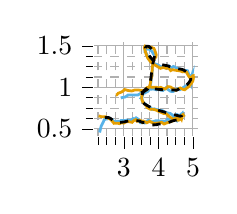
\begin{tikzpicture}

\definecolor{color0}{rgb}{1,0.188235294117647,0.188235294117647}
\definecolor{color0}{rgb}{0.90, 0.62, 0.00}
\definecolor{color1}{rgb}{0.34, 0.70, 0.91}
\definecolor{color2}{rgb}{0.00, 0.62, 0.45}
\definecolor{color3}{rgb}{0.94, 0.89, 0.27}
\definecolor{color4}{rgb}{0.00, 0.45, 0.69}
\definecolor{color5}{rgb}{0.83, 0.37, 0.00}


\begin{axis}[
    width=\figurewidth,
    height=\figureheight,
legend cell align={left},
legend style={
  fill opacity=0.8,
  draw opacity=1,
  text opacity=1,
  at={(0.97,0.03)},
  anchor=south east,
  draw=white!80!black
},
axis line style= {white},
tick align=outside,
tick pos=left,
% title={XY plot},
xmajorgrids,
xmajorticks=true,
xminorgrids,
xminorgrids=true,
ymajorgrids,
ymajorticks=true,
yminorgrids,
yminorgrids=true,
    yticklabel style={
            /pgf/number format/fixed,
            /pgf/number format/precision=5
    },
    scaled y ticks=false,
            minor tick num = 3,
        minor grid style={dashed},
x grid style={white!69.0196078431373!black},
xmin=2.12877276002231, xmax=5.16023554096054,
xtick style={color=black},
y grid style={white!69.0196078431373!black},
ymin=0.404950771684837, ymax=1.54912152663555,
ytick style={color=black}
]
\addplot [line width=1pt, color1]
table {%
2.2954216427211 0.456958533273505
2.31777733333452 0.49487950715315
2.33763132237825 0.529290846679961
2.37099891932597 0.558159603164172
2.39915270681096 0.581603031021609
2.43237971210357 0.611786834903712
2.48228843678183 0.619828840130322
2.50723591521166 0.618996725006725
2.57016757457341 0.628498933188615
2.61110224606921 0.618617386776924
2.65472841443386 0.614607834975727
2.69645540690029 0.595761471537237
2.73302168382298 0.587547656728352
2.78460398196515 0.590958649413665
2.83162000452564 0.591881436489796
2.87356750945619 0.587976674053637
2.92110874032325 0.602002696201986
2.97777074365821 0.60076945794349
3.02254324868717 0.599485724584289
3.09168373521269 0.606668274298737
3.13921476015578 0.601798888398763
3.20421169494298 0.601803934405946
3.26403626073103 0.624994661038883
3.308839878853 0.618054264314445
3.35316934072594 0.633184133508421
3.39633428969372 0.621581680741958
3.43829247711476 0.608653774943656
3.47959461117091 0.575099462250055
3.50625344126635 0.572568446543079
3.52119343091084 0.572684579097422
3.55705093628962 0.582454008587114
3.58359333367066 0.572830630436128
3.61456898100191 0.57180452551432
3.66382379414986 0.591655611703931
3.70350267599603 0.601012115979793
3.73986772656383 0.597981792655272
3.79459211832735 0.583684884156747
3.8589167167674 0.588966843957799
3.92124063459251 0.59836364931814
3.99992257838136 0.597582087944079
4.04932519277265 0.593434769797821
4.12635767857896 0.595421832362148
4.18267360064715 0.587168678823642
4.26760867678425 0.61323269863585
4.33154077984819 0.619632582003686
4.40008314812554 0.616422580950774
4.44440381051309 0.642036095741194
4.50073852441353 0.627756915178666
4.54387388862518 0.600471148141839
4.57784565316582 0.616949772980762
4.61861403199193 0.638238638834733
4.65154330276112 0.644806702267674
4.64713122150596 0.63367921735363
4.65879743126192 0.669634341593406
4.70050728512957 0.689264916110825
4.71491058954871 0.670265382912131
4.66791998111957 0.673432023045431
4.66456338564272 0.663546258504555
4.6514615485341 0.673433980979231
4.61419404518564 0.658970398827948
4.57197420706711 0.666703837043153
4.53758470508788 0.671934417412527
4.46912709671841 0.653844414067499
4.42916135383894 0.65968524912859
4.34431157821041 0.685358084016413
4.25510880352394 0.69307586205989
4.19943957942588 0.701937000010989
4.10868519659685 0.720095622449483
4.03084815122655 0.724435974931953
3.96403028690104 0.731778433289824
3.87862436703802 0.741309372872078
3.81631763394191 0.734836655091209
3.75911789075354 0.761445802916635
3.71140899378346 0.759670298112906
3.65434881455194 0.789383693822738
3.60680009805964 0.803059543989636
3.58652056216466 0.813322396882952
3.55043822523879 0.824897819019936
3.53340288012352 0.840585453207842
3.52469800454746 0.849309565324545
3.52613146215501 0.879255694390182
3.50699401464921 0.87885509882795
3.54187917205913 0.904607260521757
3.53992240245697 0.911776331357928
3.55999978636447 0.926187070720048
3.58142860940515 0.934689504021621
3.59744380239372 0.933546064274718
3.61509018467778 0.954467023878263
3.64513837855198 0.966678058414332
3.67737153279367 0.956835685894477
3.70888977791336 0.973457766206282
3.76111119411413 0.976457955699481
3.81567450582051 0.978880187295118
3.87873492581653 0.978734109121055
3.94845073923546 0.96995812975022
4.00428374323119 0.97968247290656
4.07382113314224 0.964835905435578
4.13568268890664 0.963451033157929
4.22094809638009 0.995157931634678
4.28045051725409 0.972477292621147
4.35828816630771 0.951715788645927
4.4285547032453 0.95058415575198
4.47791919068106 0.960707664166411
4.55688852191186 0.984419651304546
4.62122417091992 0.971751831612376
4.68121848605205 0.985980195289496
4.73146398329164 1.00240644796764
4.78350441257105 1.01293429952561
4.83617557570634 1.02839853580769
4.88170283359478 1.05042831139707
4.93427000544225 1.08165869271809
4.95618168663791 1.1164418127072
4.95904613541331 1.10544999991501
4.97156268814394 1.14284870029486
4.96111937046137 1.13248620425793
4.95360187519411 1.12856981396099
4.94110527615339 1.12136826430779
4.90874431955096 1.13975526380678
4.88445928190409 1.15118368116767
4.84402526283237 1.19951970322011
4.81363791051145 1.20221132249522
4.74639621909141 1.20186365755875
4.70270904061743 1.21033719632458
4.64008299046569 1.21925373592581
4.57376563144212 1.22002153597137
4.49753014236375 1.23972725018781
4.4323391667904 1.25168273938092
4.3752508721595 1.23057699533913
4.30350269834918 1.25793334385766
4.23780888271187 1.23861195945078
4.16120874459902 1.25862519873877
4.08395576213948 1.24417509580164
3.99330635987506 1.26722145795548
3.90717893497241 1.28285985998207
3.82396238528935 1.29433042920734
3.73051040945206 1.33602361791541
3.67380135412162 1.38722348527647
3.62732310185697 1.42740486735385
3.60816445200711 1.43096683264484
3.6098946166593 1.46420167865521
3.62974614417943 1.4606499087354
3.63564250016771 1.4628090494307
3.67777015015346 1.45993833472835
3.71591579123588 1.46263587920374
3.75898147583426 1.44949469574389
3.79552346889038 1.44062697468932
3.82217176546725 1.4270307741753
3.85307696350958 1.40036671651812
3.88682844445628 1.39766894649338
3.88813003946867 1.37806342977231
3.89499281734444 1.37318389131059
3.89927045065691 1.36299155725777
3.86211921707423 1.33984612380685
3.8675035459905 1.32903653727561
3.8550389843343 1.31918825508543
3.84582553031054 1.266029771924
3.82192860675603 1.23864452174203
3.8188104365502 1.20708994254779
3.81326090765918 1.14070726337675
3.79713954466694 1.11078098661924
3.77813464376112 1.04934668163039
3.76760799931913 1.02317563752568
3.73444576200688 0.97866913059187
3.70009956408722 0.953033900190684
3.64725299707619 0.941730769001205
3.57459200766659 0.928809906030269
3.49507137704457 0.928975172026874
3.40462543050264 0.908870429954832
3.31878053771735 0.906522072719271
3.21306244747252 0.906822278537671
3.11988218513941 0.907357408886252
3.03607055697764 0.883460231704356
2.95875103539358 0.878559911280428
2.90943214434925 0.871585647476596
};
% \addlegendentry{Ours }
\addplot [line width=1pt, color0]
table {%
2.26656652279223 0.657010612239058
2.35714382130048 0.645698437987604
2.46912835587662 0.646742571562861
2.54904439484317 0.62647268601071
2.61610617873149 0.615033248815969
2.67091839597072 0.587527391166454
2.71293841304514 0.566557237876796
2.8289300166783 0.56724183290176
2.8774984141375 0.562835575197254
2.9297412196155 0.574767195104584
2.99582687673874 0.569375858413319
3.04398971125765 0.580960908636404
3.11821334733149 0.589230026100572
3.23500900778058 0.578972956710099
3.29710121648793 0.602869530796653
3.34523716767429 0.610498545305097
3.38133012793502 0.592091640957174
3.42218117361351 0.596601918924841
3.46468232077013 0.605446191691559
3.50232048035524 0.59331040534939
3.53138675226301 0.578954124385501
3.56050365837881 0.593471293840019
3.5866636872793 0.587441829084113
3.61679437274807 0.585436550167668
3.66508438167831 0.574030825320271
3.71110243709038 0.583491131606597
3.74881729731915 0.590701699692942
3.87321212722207 0.565351407396609
3.94332451694098 0.569375888805397
4.02933308877975 0.573217204811524
4.09019776487595 0.578697321920415
4.16508434190537 0.558774371932346
4.22440220256894 0.570017814051165
4.30491172300629 0.580211876341465
4.45110679138145 0.601787538331989
4.49818151091311 0.616557406612546
4.54490620065661 0.606157718175345
4.58474715181891 0.603748215910125
4.61732776598191 0.612260202930852
4.64513056496436 0.623836672256871
4.68209119320882 0.639473359682488
4.67689255581475 0.656413354814575
4.71121890184527 0.671493474375941
4.72908747193449 0.660581288371215
4.68988240652772 0.651813349136982
4.67061365107596 0.619723430507855
4.66318354414061 0.625654022015665
4.62011394913901 0.616804803660629
4.52897023159987 0.633532465778361
4.45192419369431 0.618005370455619
4.40100904910164 0.622471582166816
4.31615609623814 0.648487353780215
4.22276895453488 0.682968405146507
4.1513383273049 0.685387413787086
4.06132088987714 0.701568477070616
3.91240201883462 0.729654784320017
3.83365064700832 0.736487016563697
3.76827987219866 0.735191718975739
3.71381407610171 0.747989026078135
3.67536896327288 0.757754302568014
3.62523566406642 0.787481070169994
3.57816940186485 0.808336627680076
3.53342552792813 0.837018512573694
3.51982087848909 0.857900350992185
3.51785614866331 0.87983859016243
3.52830366103386 0.914689697777957
3.51297702842778 0.91779790983678
3.54607893560372 0.942201302549024
3.56705205771726 0.96160500839244
3.60401281076548 0.968176824179276
3.62928634441175 0.977424816005104
3.64446115856433 0.98854923733403
3.67286715948425 0.997481256467301
3.71002245775272 0.999000764258679
3.74868867147703 1.00551834148556
3.80102292687833 1.00210401950882
3.93236281040655 1.00202748043467
4.00647533265346 0.991707550655818
4.06658877149959 0.999853118029554
4.13244637976297 0.987300409123901
4.1961475001081 0.980690779878946
4.27739257805573 1.00865384311342
4.34797240131824 1.00505626919742
4.49815402389132 0.964686392024289
4.55318674767089 0.975173104382569
4.63109920128498 0.992214323705194
4.70003778680557 0.977635694403429
4.76173411000382 0.970582182546276
4.80983644276065 0.98772491904037
4.85795678179988 1.00187251057426
4.94957756098052 1.04332747828965
5.00200282074395 1.08104896882526
5.02244177819062 1.13409488077488
5.01361867542625 1.12385764666774
5.01083580216477 1.14058092021073
4.99080038985157 1.13862285041618
4.97426244268442 1.12637073288414
4.92098387821703 1.11237674535651
4.89068955830255 1.12632378485632
4.85105684806315 1.15338153706751
4.81949275852938 1.1802201492966
4.75215494766644 1.189201715826
4.7000965492915 1.18631715643634
4.6370482848981 1.19710683876199
4.48600491487912 1.20630857760943
4.4143954307876 1.21285429981377
4.35508778149186 1.202070126601
4.28856147136882 1.23690657263644
4.21924292669192 1.22873410169901
4.14232480811796 1.24007702537664
4.05807420954335 1.22883324088849
3.87004989365037 1.27584502213182
3.78420504498652 1.30200693519575
3.69286429381683 1.35019264639585
3.63283440896259 1.41278413765946
3.60052766507381 1.46554881335009
3.59385470673663 1.48216535325547
3.61573660602321 1.49711376504688
3.67854550142618 1.48416807027805
3.72883539212453 1.48239981199108
3.78066445016795 1.48464560222221
3.82685738124627 1.47546689225864
3.86869615050429 1.46906545974477
3.89120954533684 1.45005143552191
3.91382799082125 1.42274324602061
3.9365317018496 1.39132730307169
3.93210645408647 1.3824463086832
3.93231502623131 1.36938887207413
3.89157036167549 1.34900145876894
3.87612959104443 1.33633294363003
3.86039258272765 1.32677290340083
3.84920205010396 1.29090759232864
3.82223804415004 1.24151728469815
3.81118702895529 1.14207346885956
3.78918835850452 1.10617092039616
3.76273740012428 1.04095998209618
3.74379930250183 1.01456959616795
3.71244778006224 0.997756247245787
3.66098633321622 0.968176820352702
3.51781356500873 0.962598085536201
3.42482929034603 0.967805219897478
3.32435618429358 0.969189952480515
3.22850809599341 0.956281648576645
3.12001769870334 0.96179460005697
3.02508054511676 0.973224968241479
2.9409249519996 0.945283145524123
2.83436894351627 0.928901271267334
2.79343853460443 0.909942415671177
2.76691028471854 0.906760277506214
};
% \addlegendentry{Point Cloud}
% \addplot [line width=1pt, green!50!black]
% table {%
% 2.35892892452518 0.675682647712128
% 2.42978630582589 0.703220041949035
% 2.48453329989567 0.711795270023535
% 2.53544276599431 0.726723723913668
% 2.60163917930246 0.727191847951841
% 2.63961579753378 0.713931684485897
% 2.70738974953776 0.702141990464947
% 2.75855673276656 0.677849089690324
% 2.8035775783111 0.655033487836737
% 2.84376380208128 0.622901863605389
% 2.8750528381069 0.58679370241161
% 2.92158934911775 0.564860313864813
% 2.97520109740467 0.564271594380181
% 3.02040086164092 0.559782760866558
% 3.06965739993503 0.565083992103844
% 3.13503458401981 0.555989880189345
% 3.1852448045617 0.563908618052208
% 3.26139294599305 0.569398247074381
% 3.31810043051243 0.560509803672526
% 3.38685611116533 0.56673625834506
% 3.45422213542551 0.591594042425316
% 3.50698442114095 0.60198713859095
% };
% \addlegendentry{Image}
\addplot [line width=1pt, black, dashed]
table {%
2.44961881637573 0.632818698883057
2.49184632301331 0.638318061828613
2.53642201423645 0.637591958045959
2.5811128616333 0.63290148973465
2.62548923492432 0.621461033821106
2.66858124732971 0.60774290561676
2.71244502067566 0.594337582588196
2.80324053764343 0.576365888118744
2.84974360466003 0.575522303581238
2.89853239059448 0.578539431095123
2.95167922973633 0.580935955047607
3.00733399391174 0.584364891052246
3.06419110298157 0.5893794298172
3.17853021621704 0.601789712905884
3.23518180847168 0.6033616065979
3.28984522819519 0.602049291133881
3.34109807014465 0.600774049758911
3.38540554046631 0.598361253738403
3.42358613014221 0.595715701580048
3.4562566280365 0.592634737491608
3.50875163078308 0.582817792892456
3.53420877456665 0.578564763069153
3.55867266654968 0.578361749649048
3.58785653114319 0.575249850749969
3.6181046962738 0.574694573879242
3.65492224693298 0.57064300775528
3.70083785057068 0.561338245868683
3.80997467041016 0.548518240451813
3.87289643287659 0.548225939273834
3.93877172470093 0.550397217273712
4.00425100326538 0.557612478733063
4.07564973831177 0.559260010719299
4.14390993118286 0.562194406986237
4.21157598495483 0.567442297935486
4.34743690490723 0.58589380979538
4.3992977142334 0.595011711120605
4.44696283340454 0.600455462932587
4.50991916656494 0.605159401893616
4.55272197723389 0.609150171279907
4.59152603149414 0.617089152336121
4.62049102783203 0.632509291172028
4.66143894195557 0.658334314823151
4.67684459686279 0.666970789432526
4.68613862991333 0.668299496173859
4.68156385421753 0.668152689933777
4.67292547225952 0.659588932991028
4.65167999267578 0.65624737739563
4.62711381912231 0.652865469455719
4.56195640563965 0.658845484256744
4.48921155929565 0.667507708072662
4.42907476425171 0.673418462276459
4.364417552948 0.681628286838531
4.28832912445068 0.689211785793304
4.21258687973022 0.697850942611694
4.13534498214722 0.707625448703766
3.9815731048584 0.725314617156982
3.91040086746216 0.734794139862061
3.84459114074707 0.744607985019684
3.83271741867065 0.745479464530945
3.83271741867065 0.745479464530945
3.59143424034119 0.801227807998657
3.59143424034119 0.801227807998657
3.55322051048279 0.819602787494659
3.53378105163574 0.835769176483154
3.52052617073059 0.853483378887177
3.51484632492065 0.872008979320526
3.51649236679077 0.889821469783783
3.52600789070129 0.904130518436432
3.53686928749084 0.918487727642059
3.56351637840271 0.944109201431274
3.57629799842834 0.957380533218384
3.59665036201477 0.966566443443298
3.62381148338318 0.975494146347046
3.65565609931946 0.986978530883789
3.696049451828 0.986358344554901
3.73732781410217 0.991490304470062
3.84776592254639 0.979946970939636
3.91309595108032 0.979255378246307
3.94392347335815 0.978964030742645
4.03354120254517 0.97417813539505
4.05302429199219 0.973176598548889
4.05302429199219 0.973176598548889
4.41191577911377 0.968668818473816
4.41191577911377 0.968668818473816
4.44498062133789 0.969216406345367
4.51591968536377 0.966148912906647
4.52946996688843 0.96590119600296
4.52946996688843 0.96590119600296
4.8422794342041 1.03704440593719
4.8422794342041 1.03704440593719
4.84621095657349 1.04014050960541
4.88337802886963 1.0569064617157
4.92765474319458 1.08610856533051
4.93645238876343 1.09527552127838
4.93645238876343 1.09527552127838
4.93231248855591 1.12826061248779
4.93231248855591 1.12826061248779
4.92480373382568 1.13175475597382
4.9000825881958 1.13904809951782
4.80996656417847 1.18516874313354
4.80996656417847 1.18516874313354
4.77510261535645 1.1967648267746
4.72225284576416 1.21030521392822
4.67178773880005 1.21736228466034
4.53933477401733 1.22587513923645
4.4741735458374 1.23063182830811
4.4066367149353 1.23750829696655
4.33526086807251 1.24806439876556
4.2646312713623 1.2597678899765
4.19270467758179 1.26518547534943
4.11613798141479 1.2717148065567
3.95782518386841 1.28673839569092
3.86118698120117 1.31957471370697
3.78020834922791 1.3553694486618
3.71509742736816 1.3904550075531
3.66681861877441 1.42694270610809
3.63695573806763 1.45624256134033
3.62501287460327 1.4771876335144
3.65587210655212 1.49541795253754
3.68864607810974 1.49557495117188
3.72396874427795 1.49183130264282
3.75977635383606 1.48014390468597
3.79366683959961 1.46717548370361
3.82296109199524 1.45282530784607
3.85447812080383 1.43851757049561
3.89113712310791 1.41326069831848
3.89532256126404 1.40173852443695
3.89313435554504 1.38950276374817
3.88669848442078 1.37267100811005
3.8734872341156 1.34983742237091
3.85793447494507 1.32186985015869
3.84170961380005 1.29361128807068
3.82747554779053 1.25897550582886
3.80352425575256 1.18452751636505
3.7911856174469 1.14020931720734
3.77538084983826 1.09253120422363
3.75537896156311 1.04756617546082
3.72709131240845 1.00902199745178
3.69070506095886 0.980598151683807
3.56822967529297 0.945891678333282
3.49198365211487 0.937991917133331
3.40586566925049 0.935832738876343
3.32272267341614 0.934732735157013
3.32272267341614 0.934732735157013
3.32272267341614 0.934732735157013
3.32272267341614 0.934732735157013
3.32272267341614 0.934732735157013
3.32272267341614 0.934732735157013
3.32272267341614 0.934732735157013
};
% \addlegendentry{GT}
\end{axis}

\end{tikzpicture}
}
        \caption{\scriptsize{YZ trajectory plot}}
        \label{fig:yz_plot}     
    \end{subfigure}
    \caption{Comparison of estimated trajectories with the point cloud tracking method and our proposed method from three different projections.}
    \label{fig:full_traj} 
\end{figure*}

\begin{figure*}[t]
    \begin{subfigure}{.32\textwidth}
        \centering
        \setlength{\figurewidth}{\textwidth}
        \setlength{\figureheight}{\textwidth}
        \scriptsize{% This file was created with tikzplotlib v0.9.14.
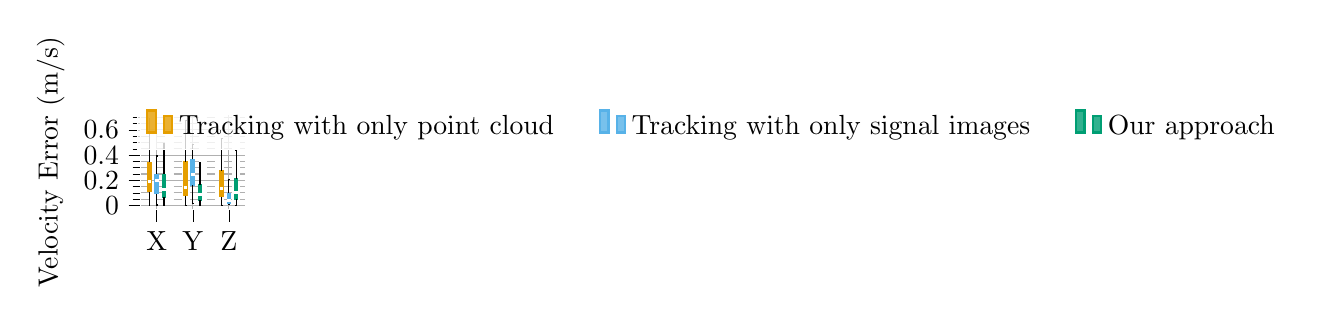
\begin{tikzpicture}

% \definecolor{color0}{rgb}{0.6,0,0.980392156862745}
% \definecolor{color1}{rgb}{0.968627450980392,0.00784313725490196,0.164705882352941}
% \definecolor{color2}{rgb}{0.0235294117647059,0.32156862745098,1}
\definecolor{color0}{rgb}{0.90, 0.62, 0.00}
\definecolor{color1}{rgb}{0.34, 0.70, 0.91}
\definecolor{color2}{rgb}{0.00, 0.62, 0.45}
\definecolor{color3}{rgb}{0.94, 0.89, 0.27}
\definecolor{color4}{rgb}{0.00, 0.45, 0.69}
\definecolor{color5}{rgb}{0.83, 0.37, 0.00}

\begin{axis}[
    width=\figurewidth,
    height=\figureheight,
legend cell align={left},
legend style={
  fill opacity=0.8,
  draw opacity=1,
  text opacity=1,
  at={(-0.03,1.12)},
  anchor=north west,
  draw=white,
/tikz/every even column/.append style={column sep=0.5cm},
},
legend columns = 3, 
axis line style={white},
tick align=outside,
tick pos=left,
% title={Seq 1 },
x grid style={white!69.0196078431373!black},
xmin=0.5, xmax=6.3,
xtick style={color=black},
xtick={1.4,3.4,5.4},
xticklabels={X,Y,Z},
y grid style={white!69.0196078431373!black},
ylabel={Velocity Error (m/s)},
ymin=-0.034208951695738, ymax=0.721221921251871,
ytick style={color=black},
    xmajorgrids,
    % xmajorticks=true,
    % xmin=-0.5, xmax=3.3125,
    xminorgrids,
    ymajorgrids,
    ymajorticks=true,
    minor y tick num = 3,
    minor y grid style={dashed},
    yminorgrids,
    yticklabel style={
            /pgf/number format/fixed,
            /pgf/number format/precision=5
    },
    scaled y ticks=false,
]

\draw[draw=color0,fill=color0, thick] (axis cs:0,0) rectangle (axis cs:0,0);
\addlegendimage{ybar, ybar legend, draw=color0,fill=color0,thick}
\addlegendentry{Tracking with only point cloud}

\draw[draw=color1,fill=color1, thick] (axis cs:0,0) rectangle (axis cs:0,0);
\addlegendimage{ybar, ybar legend, draw=color1,fill=color1,thick}
\addlegendentry{Tracking with only signal images}

\draw[draw=color2,fill=color2, thick] (axis cs:0,0) rectangle (axis cs:0,0);
\addlegendimage{ybar, ybar legend, draw=color2,fill=color2,thick}
\addlegendentry{Our approach}

\path [draw=color0, fill=color0]
(axis cs:0.9,0.109162671124885)
--(axis cs:1.1,0.109162671124885)
--(axis cs:1.1,0.344490432716165)
--(axis cs:0.9,0.344490432716165)
--(axis cs:0.9,0.109162671124885)
--cycle;
\addplot [black, forget plot]
table {%
1 0.109162671124885
1 0.000128815256426051
};
\addplot [black, forget plot]
table {%
1 0.344490432716165
1 0.686884154299707
};
\addplot [black, forget plot]
table {%
0.95 0.000128815256426051
1.05 0.000128815256426051
};
\addplot [black, forget plot]
table {%
0.95 0.686884154299707
1.05 0.686884154299707
};
\path [draw=color1, fill=color1]
(axis cs:1.3,0.0919291443556336)
--(axis cs:1.5,0.0919291443556336)
--(axis cs:1.5,0.24845085936301)
--(axis cs:1.3,0.24845085936301)
--(axis cs:1.3,0.0919291443556336)
--cycle;
\addplot [black, forget plot]
table {%
1.4 0.0919291443556336
1.4 0.00361160361343593
};
\addplot [black, forget plot]
table {%
1.4 0.24845085936301
1.4 0.392370148027017
};
\addplot [black, forget plot]
table {%
1.35 0.00361160361343593
1.45 0.00361160361343593
};
\addplot [black, forget plot]
table {%
1.35 0.392370148027017
1.45 0.392370148027017
};
\path [draw=color2, fill=color2]
(axis cs:1.7,0.0651457039411474)
--(axis cs:1.9,0.0651457039411474)
--(axis cs:1.9,0.248436061039956)
--(axis cs:1.7,0.248436061039956)
--(axis cs:1.7,0.0651457039411474)
--cycle;
\addplot [black, forget plot]
table {%
1.8 0.0651457039411474
1.8 0.0027373277432563
};
\addplot [black, forget plot]
table {%
1.8 0.248436061039956
1.8 0.493909091734377
};
\addplot [black, forget plot]
table {%
1.75 0.0027373277432563
1.85 0.0027373277432563
};
\addplot [black, forget plot]
table {%
1.75 0.493909091734377
1.85 0.493909091734377
};
\path [draw=color0, fill=color0]
(axis cs:2.9,0.0771871383898404)
--(axis cs:3.1,0.0771871383898404)
--(axis cs:3.1,0.347491246148062)
--(axis cs:2.9,0.347491246148062)
--(axis cs:2.9,0.0771871383898404)
--cycle;
\addplot [black, forget plot]
table {%
3 0.0771871383898404
3 0.000199890722223373
};
\addplot [black, forget plot]
table {%
3 0.347491246148062
3 0.677734254757247
};
\addplot [black, forget plot]
table {%
2.95 0.000199890722223373
3.05 0.000199890722223373
};
\addplot [black, forget plot]
table {%
2.95 0.677734254757247
3.05 0.677734254757247
};
\path [draw=color1, fill=color1]
(axis cs:3.3,0.158876445092808)
--(axis cs:3.5,0.158876445092808)
--(axis cs:3.5,0.366330405403881)
--(axis cs:3.3,0.366330405403881)
--(axis cs:3.3,0.158876445092808)
--cycle;
\addplot [black, forget plot]
table {%
3.4 0.158876445092808
3.4 0.0153142890715063
};
\addplot [black, forget plot]
table {%
3.4 0.366330405403881
3.4 0.486702403844719
};
\addplot [black, forget plot]
table {%
3.35 0.0153142890715063
3.45 0.0153142890715063
};
\addplot [black, forget plot]
table {%
3.35 0.486702403844719
3.45 0.486702403844719
};
\path [draw=color2, fill=color2]
(axis cs:3.7,0.0411681137598663)
--(axis cs:3.9,0.0411681137598663)
--(axis cs:3.9,0.163136180242405)
--(axis cs:3.7,0.163136180242405)
--(axis cs:3.7,0.0411681137598663)
--cycle;
\addplot [black, forget plot]
table {%
3.8 0.0411681137598663
3.8 0.000443114872510364
};
\addplot [black, forget plot]
table {%
3.8 0.163136180242405
3.8 0.342459269664861
};
\addplot [black, forget plot]
table {%
3.75 0.000443114872510364
3.85 0.000443114872510364
};
\addplot [black, forget plot]
table {%
3.75 0.342459269664861
3.85 0.342459269664861
};
\path [draw=color0, fill=color0]
(axis cs:4.9,0.070570502146341)
--(axis cs:5.1,0.070570502146341)
--(axis cs:5.1,0.276398234476372)
--(axis cs:4.9,0.276398234476372)
--(axis cs:4.9,0.070570502146341)
--cycle;
\addplot [black, forget plot]
table {%
5 0.070570502146341
5 0.000259953570465044
};
\addplot [black, forget plot]
table {%
5 0.276398234476372
5 0.531454865660448
};
\addplot [black, forget plot]
table {%
4.95 0.000259953570465044
5.05 0.000259953570465044
};
\addplot [black, forget plot]
table {%
4.95 0.531454865660448
5.05 0.531454865660448
};
\path [draw=color1, fill=color1]
(axis cs:5.3,0.0136535369876245)
--(axis cs:5.5,0.0136535369876245)
--(axis cs:5.5,0.0975762615115577)
--(axis cs:5.3,0.0975762615115577)
--(axis cs:5.3,0.0136535369876245)
--cycle;
\addplot [black, forget plot]
table {%
5.4 0.0136535369876245
5.4 0.00456348111469773
};
\addplot [black, forget plot]
table {%
5.4 0.0975762615115577
5.4 0.209099309075048
};
\addplot [black, forget plot]
table {%
5.35 0.00456348111469773
5.45 0.00456348111469773
};
\addplot [black, forget plot]
table {%
5.35 0.209099309075048
5.45 0.209099309075048
};
\path [draw=color2, fill=color2]
(axis cs:5.7,0.051383654669091)
--(axis cs:5.9,0.051383654669091)
--(axis cs:5.9,0.210674396423683)
--(axis cs:5.7,0.210674396423683)
--(axis cs:5.7,0.051383654669091)
--cycle;
\addplot [black, forget plot]
table {%
5.8 0.051383654669091
5.8 0.000249636769975581
};
\addplot [black, forget plot]
table {%
5.8 0.210674396423683
5.8 0.438200065621051
};
\addplot [black, forget plot]
table {%
5.75 0.000249636769975581
5.85 0.000249636769975581
};
\addplot [black, forget plot]
table {%
5.75 0.438200065621051
5.85 0.438200065621051
};
\addplot [line width=1pt, white, forget plot]
table {%
0.9 0.191737841303157
1.1 0.191737841303157
};
\addplot [line width=1pt, white, forget plot]
table {%
1.3 0.197800169460929
1.5 0.197800169460929
};
\addplot [line width=1pt, white, forget plot]
table {%
1.7 0.128881545706658
1.9 0.128881545706658
};
\addplot [line width=1pt, white, forget plot]
table {%
2.9 0.141984442865786
3.1 0.141984442865786
};
\addplot [line width=1pt, white, forget plot]
table {%
3.3 0.247618886526242
3.5 0.247618886526242
};
\addplot [line width=1pt, white, forget plot]
table {%
3.7 0.0878626303248753
3.9 0.0878626303248753
};
\addplot [line width=1pt, white, forget plot]
table {%
4.9 0.134968087815255
5.1 0.134968087815255
};
\addplot [line width=1pt, white, forget plot]
table {%
5.3 0.0402095843975281
5.5 0.0402095843975281
};
\addplot [line width=1pt, white, forget plot]
table {%
5.7 0.105071468625511
5.9 0.105071468625511
};
\end{axis}

\end{tikzpicture}
}
        \caption{\scriptsize{Seq\,1}}
        \label{fig:vel_err_seq1}
    \end{subfigure}
    \hfill
    \begin{subfigure}{.32\textwidth}
        \centering
        \setlength{\figurewidth}{\textwidth}
        \setlength{\figureheight}{\textwidth}
        \scriptsize{% This file was created with tikzplotlib v0.9.14.
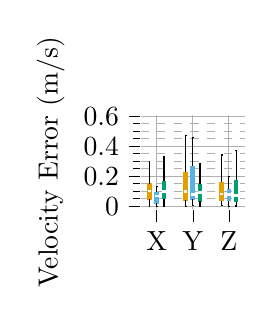
\begin{tikzpicture}

% \definecolor{color0}{rgb}{0.6,0,0.980392156862745}
% \definecolor{color1}{rgb}{0.968627450980392,0.00784313725490196,0.164705882352941}
% \definecolor{color2}{rgb}{0.0235294117647059,0.32156862745098,1}
\definecolor{color0}{rgb}{0.90, 0.62, 0.00}
\definecolor{color1}{rgb}{0.34, 0.70, 0.91}
\definecolor{color2}{rgb}{0.00, 0.62, 0.45}
\definecolor{color3}{rgb}{0.94, 0.89, 0.27}
\definecolor{color4}{rgb}{0.00, 0.45, 0.69}
\definecolor{color5}{rgb}{0.83, 0.37, 0.00}

\begin{axis}[
    width=\figurewidth,
    height=\figureheight,
legend cell align={left},
legend style={
  fill opacity=0.8,
  draw opacity=1,
  text opacity=1,
  at={(0.03,0.97)},
  anchor=north west,
  draw=white!80!black
},
axis line style={white},
tick align=outside,
tick pos=left,
% title={Seq 2 },
x grid style={white!69.0196078431373!black},
xmin=0.5, xmax=6.3,
xtick style={color=black},
xtick={1.4,3.4,5.4},
xticklabels={X,Y,Z},
y grid style={white!69.0196078431373!black},
ylabel={Velocity Error (m/s)},
ymin=-0.0233556679147973, ymax=0.61,
ytick style={color=black},
    xmajorgrids,
    % xmajorticks=true,
    % xmin=-0.5, xmax=3.3125,
    xminorgrids,
    ymajorgrids,
    ymajorticks=true,
    minor y tick num = 3,
    minor y grid style={dashed},
    yminorgrids,
    yticklabel style={
            /pgf/number format/fixed,
            /pgf/number format/precision=5
    },
    scaled y ticks=false,
]
\path [draw=color0, fill=color0]
(axis cs:0.9,0.0454993116751612)
--(axis cs:1.1,0.0454993116751612)
--(axis cs:1.1,0.149575866732583)
--(axis cs:0.9,0.149575866732583)
--(axis cs:0.9,0.0454993116751612)
--cycle;
\addplot [black, forget plot]
table {%
1 0.0454993116751612
1 0.000176190755700745
};
\addplot [black, forget plot]
table {%
1 0.149575866732583
1 0.298551854208258
};
\addplot [black, forget plot]
table {%
0.95 0.000176190755700745
1.05 0.000176190755700745
};
\addplot [black, forget plot]
table {%
0.95 0.298551854208258
1.05 0.298551854208258
};
\path [draw=color1, fill=color1]
(axis cs:1.3,0.0193088946071396)
--(axis cs:1.5,0.0193088946071396)
--(axis cs:1.5,0.0943910742063947)
--(axis cs:1.3,0.0943910742063947)
--(axis cs:1.3,0.0193088946071396)
--cycle;
\addplot [black, forget plot]
table {%
1.4 0.0193088946071396
1.4 0.000377116058847271
};
\addplot [black, forget plot]
table {%
1.4 0.0943910742063947
1.4 0.132937731845124
};
\addplot [black, forget plot]
table {%
1.35 0.000377116058847271
1.45 0.000377116058847271
};
\addplot [black, forget plot]
table {%
1.35 0.132937731845124
1.45 0.132937731845124
};
\path [draw=color2, fill=color2]
(axis cs:1.7,0.0512629607750226)
--(axis cs:1.9,0.0512629607750226)
--(axis cs:1.9,0.165225579088091)
--(axis cs:1.7,0.165225579088091)
--(axis cs:1.7,0.0512629607750226)
--cycle;
\addplot [black, forget plot]
table {%
1.8 0.0512629607750226
1.8 0.00075650953687223
};
\addplot [black, forget plot]
table {%
1.8 0.165225579088091
1.8 0.332121025821897
};
\addplot [black, forget plot]
table {%
1.75 0.00075650953687223
1.85 0.00075650953687223
};
\addplot [black, forget plot]
table {%
1.75 0.332121025821897
1.85 0.332121025821897
};
\path [draw=color0, fill=color0]
(axis cs:2.9,0.0417637473191679)
--(axis cs:3.1,0.0417637473191679)
--(axis cs:3.1,0.224785137712553)
--(axis cs:2.9,0.224785137712553)
--(axis cs:2.9,0.0417637473191679)
--cycle;
\addplot [black, forget plot]
table {%
3 0.0417637473191679
3 0.000264292467084815
};
\addplot [black, forget plot]
table {%
3 0.224785137712553
3 0.470813364165661
};
\addplot [black, forget plot]
table {%
2.95 0.000264292467084815
3.05 0.000264292467084815
};
\addplot [black, forget plot]
table {%
2.95 0.470813364165661
3.05 0.470813364165661
};
\path [draw=color1, fill=color1]
(axis cs:3.3,0.0448127976552481)
--(axis cs:3.5,0.0448127976552481)
--(axis cs:3.5,0.266378868864894)
--(axis cs:3.3,0.266378868864894)
--(axis cs:3.3,0.0448127976552481)
--cycle;
\addplot [black, forget plot]
table {%
3.4 0.0448127976552481
3.4 0.00411012798469557
};
\addplot [black, forget plot]
table {%
3.4 0.266378868864894
3.4 0.456005566679127
};
\addplot [black, forget plot]
table {%
3.35 0.00411012798469557
3.45 0.00411012798469557
};
\addplot [black, forget plot]
table {%
3.35 0.456005566679127
3.45 0.456005566679127
};
\path [draw=color2, fill=color2]
(axis cs:3.7,0.032206746853467)
--(axis cs:3.9,0.032206746853467)
--(axis cs:3.9,0.147270781441821)
--(axis cs:3.7,0.147270781441821)
--(axis cs:3.7,0.032206746853467)
--cycle;
\addplot [black, forget plot]
table {%
3.8 0.032206746853467
3.8 0.00140957279476162
};
\addplot [black, forget plot]
table {%
3.8 0.147270781441821
3.8 0.285432958940515
};
\addplot [black, forget plot]
table {%
3.75 0.00140957279476162
3.85 0.00140957279476162
};
\addplot [black, forget plot]
table {%
3.75 0.285432958940515
3.85 0.285432958940515
};
\path [draw=color0, fill=color0]
(axis cs:4.9,0.0365176475868445)
--(axis cs:5.1,0.0365176475868445)
--(axis cs:5.1,0.159425725571298)
--(axis cs:4.9,0.159425725571298)
--(axis cs:4.9,0.0365176475868445)
--cycle;
\addplot [black, forget plot]
table {%
5 0.0365176475868445
5 0.00350969869741924
};
\addplot [black, forget plot]
table {%
5 0.159425725571298
5 0.341189883516642
};
\addplot [black, forget plot]
table {%
4.95 0.00350969869741924
5.05 0.00350969869741924
};
\addplot [black, forget plot]
table {%
4.95 0.341189883516642
5.05 0.341189883516642
};
\path [draw=color1, fill=color1]
(axis cs:5.3,0.0352932972645825)
--(axis cs:5.5,0.0352932972645825)
--(axis cs:5.5,0.111943745306393)
--(axis cs:5.3,0.111943745306393)
--(axis cs:5.3,0.0352932972645825)
--cycle;
\addplot [black, forget plot]
table {%
5.4 0.0352932972645825
5.4 0.000227750891903522
};
\addplot [black, forget plot]
table {%
5.4 0.111943745306393
5.4 0.195521128516952
};
\addplot [black, forget plot]
table {%
5.35 0.000227750891903522
5.45 0.000227750891903522
};
\addplot [black, forget plot]
table {%
5.35 0.195521128516952
5.45 0.195521128516952
};
\path [draw=color2, fill=color2]
(axis cs:5.7,0.0305767420525668)
--(axis cs:5.9,0.0305767420525668)
--(axis cs:5.9,0.172522100116694)
--(axis cs:5.7,0.172522100116694)
--(axis cs:5.7,0.0305767420525668)
--cycle;
\addplot [black, forget plot]
table {%
5.8 0.0305767420525668
5.8 0.00128623420413865
};
\addplot [black, forget plot]
table {%
5.8 0.172522100116694
5.8 0.369336006006802
};
\addplot [black, forget plot]
table {%
5.75 0.00128623420413865
5.85 0.00128623420413865
};
\addplot [black, forget plot]
table {%
5.75 0.369336006006802
5.85 0.369336006006802
};
\addplot [line width=1pt, white, forget plot]
table {%
0.9 0.100766256788645
1.1 0.100766256788645
};
\addplot [line width=1pt, white, forget plot]
table {%
1.3 0.0682491611946423
1.5 0.0682491611946423
};
\addplot [line width=1pt, white, forget plot]
table {%
1.7 0.099464031339338
1.9 0.099464031339338
};
\addplot [line width=1pt, white, forget plot]
table {%
2.9 0.0989566119088892
3.1 0.0989566119088892
};
\addplot [line width=1pt, white, forget plot]
table {%
3.3 0.075984746026001
3.5 0.075984746026001
};
\addplot [line width=1pt, white, forget plot]
table {%
3.7 0.0908502564243308
3.9 0.0908502564243308
};
\addplot [line width=1pt, white, forget plot]
table {%
4.9 0.0821778973760645
5.1 0.0821778973760645
};
\addplot [line width=1pt, white, forget plot]
table {%
5.3 0.079976425217278
5.5 0.079976425217278
};
\addplot [line width=1pt, white, forget plot]
table {%
5.7 0.0728472717659245
5.9 0.0728472717659245
};
\end{axis}

\end{tikzpicture}
}
        \caption{\scriptsize{Seq\,2}}
        \label{fig:vel_err_seq2}     
    \end{subfigure}
    \hfill
    \begin{subfigure}{.32\textwidth}
        \centering
        \setlength{\figurewidth}{\textwidth}
        \setlength{\figureheight}{\textwidth}
        \scriptsize{% This file was created with tikzplotlib v0.9.14.
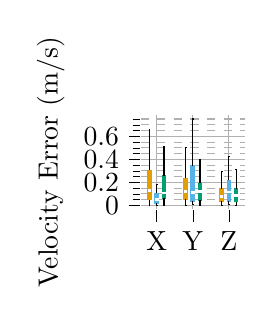
\begin{tikzpicture}

% \definecolor{color0}{rgb}{0.6,0,0.980392156862745}
% \definecolor{color1}{rgb}{0.968627450980392,0.00784313725490196,0.164705882352941}
% \definecolor{color2}{rgb}{0.0235294117647059,0.32156862745098,1}
\definecolor{color0}{rgb}{0.90, 0.62, 0.00}
\definecolor{color1}{rgb}{0.34, 0.70, 0.91}
\definecolor{color2}{rgb}{0.00, 0.62, 0.45}
\definecolor{color3}{rgb}{0.94, 0.89, 0.27}
\definecolor{color4}{rgb}{0.00, 0.45, 0.69}
\definecolor{color5}{rgb}{0.83, 0.37, 0.00}

\begin{axis}[
    width=\figurewidth,
    height=\figureheight,
legend cell align={left},
legend style={
  fill opacity=0.8,
  draw opacity=1,
  text opacity=1,
  at={(0.03,0.97)},
  anchor=north west,
  draw=white!80!black
},
axis line style={white},
tick align=outside,
tick pos=left,
% title={Seq 3 },
x grid style={white!69.0196078431373!black},
xmin=0.5, xmax=6.3,
xtick style={color=black},
xtick={1.4,3.4,5.4},
xticklabels={X,Y,Z},
y grid style={white!69.0196078431373!black},
ylabel={Velocity Error (m/s)},
ymin=-0.0375045054404742, ymax=0.78781873238659,
ytick style={color=black},
    xmajorgrids,
    % xmajorticks=true,
    % xmin=-0.5, xmax=3.3125,
    xminorgrids,
    ymajorgrids,
    ymajorticks=true,
    minor y tick num = 3,
    minor y grid style={dashed},
    yminorgrids,
    yticklabel style={
            /pgf/number format/fixed,
            /pgf/number format/precision=5
    },
    scaled y ticks=false,
]
\path [draw=color0, fill=color0]
(axis cs:0.9,0.050925850163972)
--(axis cs:1.1,0.050925850163972)
--(axis cs:1.1,0.305209551337428)
--(axis cs:0.9,0.305209551337428)
--(axis cs:0.9,0.050925850163972)
--cycle;
\addplot [black, forget plot]
table {%
1 0.050925850163972
1 0.000915280434687915
};
\addplot [black, forget plot]
table {%
1 0.305209551337428
1 0.658851716939473
};
\addplot [black, forget plot]
table {%
0.95 0.000915280434687915
1.05 0.000915280434687915
};
\addplot [black, forget plot]
table {%
0.95 0.658851716939473
1.05 0.658851716939473
};
\path [draw=color1, fill=color1]
(axis cs:1.3,0.0186842481424454)
--(axis cs:1.5,0.0186842481424454)
--(axis cs:1.5,0.103976060431693)
--(axis cs:1.3,0.103976060431693)
--(axis cs:1.3,0.0186842481424454)
--cycle;
\addplot [black, forget plot]
table {%
1.4 0.0186842481424454
1.4 0.000318754243475716
};
\addplot [black, forget plot]
table {%
1.4 0.103976060431693
1.4 0.180866270180915
};
\addplot [black, forget plot]
table {%
1.35 0.000318754243475716
1.45 0.000318754243475716
};
\addplot [black, forget plot]
table {%
1.35 0.180866270180915
1.45 0.180866270180915
};
\path [draw=color2, fill=color2]
(axis cs:1.7,0.0607938102103689)
--(axis cs:1.9,0.0607938102103689)
--(axis cs:1.9,0.255498452503433)
--(axis cs:1.7,0.255498452503433)
--(axis cs:1.7,0.0607938102103689)
--cycle;
\addplot [black, forget plot]
table {%
1.8 0.0607938102103689
1.8 0.000215207845459808
};
\addplot [black, forget plot]
table {%
1.8 0.255498452503433
1.8 0.509395351885571
};
\addplot [black, forget plot]
table {%
1.75 0.000215207845459808
1.85 0.000215207845459808
};
\addplot [black, forget plot]
table {%
1.75 0.509395351885571
1.85 0.509395351885571
};
\path [draw=color0, fill=color0]
(axis cs:2.9,0.0540813292258191)
--(axis cs:3.1,0.0540813292258191)
--(axis cs:3.1,0.234681439454613)
--(axis cs:2.9,0.234681439454613)
--(axis cs:2.9,0.0540813292258191)
--cycle;
\addplot [black, forget plot]
table {%
3 0.0540813292258191
3 0.00025457195519607
};
\addplot [black, forget plot]
table {%
3 0.234681439454613
3 0.50483313777927
};
\addplot [black, forget plot]
table {%
2.95 0.00025457195519607
3.05 0.00025457195519607
};
\addplot [black, forget plot]
table {%
2.95 0.50483313777927
3.05 0.50483313777927
};
\path [draw=color1, fill=color1]
(axis cs:3.3,0.0341207415404121)
--(axis cs:3.5,0.0341207415404121)
--(axis cs:3.5,0.341801049261369)
--(axis cs:3.3,0.341801049261369)
--(axis cs:3.3,0.0341207415404121)
--cycle;
\addplot [black, forget plot]
table {%
3.4 0.0341207415404121
3.4 0.00729099756574314
};
\addplot [black, forget plot]
table {%
3.4 0.341801049261369
3.4 0.750304039758087
};
\addplot [black, forget plot]
table {%
3.35 0.00729099756574314
3.45 0.00729099756574314
};
\addplot [black, forget plot]
table {%
3.35 0.750304039758087
3.45 0.750304039758087
};
\path [draw=color2, fill=color2]
(axis cs:3.7,0.0470434830938093)
--(axis cs:3.9,0.0470434830938093)
--(axis cs:3.9,0.190534730347155)
--(axis cs:3.7,0.190534730347155)
--(axis cs:3.7,0.0470434830938093)
--cycle;
\addplot [black, forget plot]
table {%
3.8 0.0470434830938093
3.8 0.000923772653984578
};
\addplot [black, forget plot]
table {%
3.8 0.190534730347155
3.8 0.397895565899473
};
\addplot [black, forget plot]
table {%
3.75 0.000923772653984578
3.85 0.000923772653984578
};
\addplot [black, forget plot]
table {%
3.75 0.397895565899473
3.85 0.397895565899473
};
\path [draw=color0, fill=color0]
(axis cs:4.9,0.0370850724055838)
--(axis cs:5.1,0.0370850724055838)
--(axis cs:5.1,0.144242538996679)
--(axis cs:4.9,0.144242538996679)
--(axis cs:4.9,0.0370850724055838)
--cycle;
\addplot [black, forget plot]
table {%
5 0.0370850724055838
5 1.01871880286986e-05
};
\addplot [black, forget plot]
table {%
5 0.144242538996679
5 0.29127738534024
};
\addplot [black, forget plot]
table {%
4.95 1.01871880286986e-05
5.05 1.01871880286986e-05
};
\addplot [black, forget plot]
table {%
4.95 0.29127738534024
5.05 0.29127738534024
};
\path [draw=color1, fill=color1]
(axis cs:5.3,0.0345189067087442)
--(axis cs:5.5,0.0345189067087442)
--(axis cs:5.5,0.216801981745139)
--(axis cs:5.3,0.216801981745139)
--(axis cs:5.3,0.0345189067087442)
--cycle;
\addplot [black, forget plot]
table {%
5.4 0.0345189067087442
5.4 0.00468124038173312
};
\addplot [black, forget plot]
table {%
5.4 0.216801981745139
5.4 0.421482532405152
};
\addplot [black, forget plot]
table {%
5.35 0.00468124038173312
5.45 0.00468124038173312
};
\addplot [black, forget plot]
table {%
5.35 0.421482532405152
5.45 0.421482532405152
};
\path [draw=color2, fill=color2]
(axis cs:5.7,0.0333654972375574)
--(axis cs:5.9,0.0333654972375574)
--(axis cs:5.9,0.145628655344953)
--(axis cs:5.7,0.145628655344953)
--(axis cs:5.7,0.0333654972375574)
--cycle;
\addplot [black, forget plot]
table {%
5.8 0.0333654972375574
5.8 0.000549304948028739
};
\addplot [black, forget plot]
table {%
5.8 0.145628655344953
5.8 0.312894917001754
};
\addplot [black, forget plot]
table {%
5.75 0.000549304948028739
5.85 0.000549304948028739
};
\addplot [black, forget plot]
table {%
5.75 0.312894917001754
5.85 0.312894917001754
};
\addplot [line width=1pt, white, forget plot]
table {%
0.9 0.129738371745527
1.1 0.129738371745527
};
\addplot [line width=1pt, white, forget plot]
table {%
1.3 0.0536968219671419
1.5 0.0536968219671419
};
\addplot [line width=1pt, white, forget plot]
table {%
1.7 0.107509878653638
1.9 0.107509878653638
};
\addplot [line width=1pt, white, forget plot]
table {%
2.9 0.121060592272317
3.1 0.121060592272317
};
\addplot [line width=1pt, white, forget plot]
table {%
3.3 0.109664642493887
3.5 0.109664642493887
};
\addplot [line width=1pt, white, forget plot]
table {%
3.7 0.119131419941609
3.9 0.119131419941609
};
\addplot [line width=1pt, white, forget plot]
table {%
4.9 0.0768678127111805
5.1 0.0768678127111805
};
\addplot [line width=1pt, white, forget plot]
table {%
5.3 0.115904482344118
5.5 0.115904482344118
};
\addplot [line width=1pt, white, forget plot]
table {%
5.7 0.083997795576003
5.9 0.083997795576003
};
\end{axis}

\end{tikzpicture}
}
        \caption{\scriptsize{Seq\,3}}
        \label{fig:vel_err_seq3}     
    \end{subfigure}
    \caption{Velocity estimation error for each linear component in the three data sequences.}
    \label{fig:vel_errs} 
\end{figure*}


\section{Experimental Results}

In this section, we report the experimental results, based on the three data sequences gathered in the indoor test environment. 

\subsection{UAV in the Ouster LiDAR point cloud}

The first parameter to analyze is the number of points that reflect from the UAV at different distances. Our analysis, shown in Fig~\ref{fig:pcd_frame}, reveals that the point cloud structure generated by the UAV is significantly influenced by the distance from the target. At short distances, the point cloud produced by LiDAR is abundant and presents comprehensive details. When the distance extends to a medium range, the number of UAV point clouds decreases to less than 100, but the three-dimensional structure of the UAV remains discernible. However, when the distance is at a medium range of 7\,m according to our results, the number of UAV point clouds reduces to single digits, and the point cloud structure becomes highly unpredictable and unstructured. It is worth noting that in a more realistic application, additional elements such as other sensor payloads or a cargo bay would potentially increase significantly the reflective surface of the UAV. 



\subsection{Trajectory Validation}

We also show a quantitative analysis of the APE based on ground truth, with the main results summarized in Fig.~\ref{fig:ape_error}. To ensure the trajectories are compared under the same coordinates, we utilize the coordinates of the ground truth as the reference coordinates and convert all trajectories generated by the three UAV tracking methods to these coordinates. 
% For the primary evaluation metric, we employ the absolute pose error (APE) [29]. To compute the error for each trajectory, we use the open-source EVO toolset. This enables us to conduct a comprehensive evaluation of the accuracy of each tracking method.
Table~\ref{tab:methods_compare} presents a comprehensive comparison of three different UAV tracking methods in terms of detectable distance, average APE, algorithm update frequency, and need for initial conditions. 
\begin{table}[h]
    \centering
    \caption{ Performance( Detectable distance, frame rate, and APE error) and initial conditions comparison of selected tracking methods. } 
    % \renewcommand{\arraystretch}{1.4}
    \resizebox{0.48\textwidth}{!}{%
    \begin{tabular}{@{}lcccc@{}}
        \toprule
        & \textbf{Distance} & \textbf{APE Error(Mean/RMSE)} & \textbf{FPS} & \textbf{ Initialization} \\ 
        & \textit{(m)} & (m) & (Hz) \\
        \midrule
        \textbf{Tracking with point cloud} & \textbf{8.0}  & 0.104 / 0.142 & 8.3  & Yes  \\
        \textbf{Tracking with signal images} & 2.4  & 0.078 / 0.088 & \textbf{10} & No \\
        \textbf{Fused(Ours)} & \textbf{8.0}  & \textbf{0.061 / 0.067} & \textbf{10} & No \\
        \bottomrule
    \end{tabular}
    }
    \label{tab:methods_compare}
\end{table}

The image-based UAV tracking method shows a relatively small average error; however, its overall error distribution is inconsistent, as the Y-axis error in the \textit{Seq\,1} sequence reaches up to 0.3\,m. Conversely, the point cloud-based UAV tracking method has the largest average error, but its error distribution is more uniform. Our proposed method, on the other hand, achieves the smallest average error and minimal error fluctuation. Additionally, to supplement the quantitative trajectory analysis, we also provide a visualization of the trajectories based on the point cloud tracking method and our proposed method from three different viewpoints, as illustrated in Fig~\ref{fig:full_traj}, with more consistent behavior.


\subsection{Velocity Validation}

In addition to pose estimation, we conducted a quantitative analysis of the UAV velocities based on the ground truth data and compared them with different UAV tracking methods. Fig.~\ref{fig:vel_errs} illustrates the velocity errors of each method along the X, Y, and Z axes. The experimental results reveal that all methods have similar mean values of the velocity errors, but different fluctuations. The image tracking method has a large fluctuation in the Y-axis velocity error, reaching up to \textit{0.75 m/s} in \textit{Seq\,3}. The point cloud tracking method also has relatively large fluctuations in all dimensions. In contrast, our method achieves smaller overall velocity errors in both the mean value and fluctuation range.

\subsection{Resource Consumption}
% To validate the performance of our UAV tracking design and better understand its limitations, we collected three flight trajectory sequences (\textit{Seq 1}, \textit{Seq 2}, and \textit{Seq 3}) in a large open area of 10 x 10 square meters, 0.5 to 8 meters away from the LiDAR scanner, as detailed in Table~\ref{tab:sequence_detail}. \textit{Seq 1} and \textit{Seq 3} represent a helical ascension trajectory, while \textit{Seq 2} represents an elliptical trajectory. We first focused on analyzing \textit{Seq 3} and compared it to the ground truth trajectory obtained from the Mocap system. 

% We conducted the experiment on two different platforms, the Lenovo Legion Y7000P equipped with 16GB RAM, 6-core Intel i5-9300H (2.40GHz) and Nvidia GTX 1660Ti (1536 CUDA cores, 6GB VRAM), as well as the commonly used embedded computing platform Jetson Nano with 4-core ARM A57 64-bit CPU (1.43GHz), 4GB RAM, and 128-core Maxwell GPU. 
Both the Intel laptop and the Jetson Nano run ROS Melodic on Ubuntu 18.04. The CPU and memory utilization is measured with a ROS resource monitor tool~\footnote{\href{https://github.com/alspitz/cpu_monitor}{https://github.com/alspitz/cpu\_monitor}}. Additionally, for minimizing the difference of the operating environment, we unified the dependencies used in each method into same version. The results are summarized in Table~\ref{tab:runtime_src}.

The memory utilization of each selected method was roughly equivalent in both processor architecture platforms. However, the same algorithm showed generally higher CPU utilization and achieved the highest publishing rate when running on the Intel processor. For the Intel processor, the point cloud tracking method had higher CPU utilization than other methods but the lowest publishing rate. The fusion method performed well on the laptop and had the smallest overall error. On the embedded computing platform, the CPU utilization of all methods did not differ significantly, and the point cloud tracking method had the lowest memory utilization but the lowest pose publication rate. The difference in CPU utilization is caused by the use of CUDA GPU acceleration in the Open3D binaries utilized for the Jetson Nano platform, while the Intel computer uses only the CPU for point cloud data processing. The image processing also leverages the embedded GPU in the Jetson Nano board. Because of the small ROI that we extract to process the point cloud, the fused method adds little overhead on top of the vision-only method.

\begin{table}[t]
    \centering
    \caption{ Average run-time resource (CPU/RAM) utilization and performance (pose calculation speed) comparison of selected tracking methods across multiple platforms. CPU utilization of 100\% equals one full processor core. } 
    % \renewcommand{\arraystretch}{1.6}
    % \resizebox{\linewidth}{!}{%
    \begin{tabular}{@{}lcc@{}}
        \toprule
         & Laptop & Jetson Nano  \\
        & \multicolumn{2}{c}{\textit{( CPU (\%), RAM (MB), Pose rate (Hz) )}} \\%[-.21em]
        \midrule
        \textbf{Tracking with point cloud} & (422.7, 296.1, 8.3 ) & (121.7, 179.7, 5.15 )  \\
        \textbf{Tracking with image} & (209.0, 293.6, 10 ) & (113.8, 232.9, 6.07)   \\
        \textbf{Fused (ours)} & (195.5, 299.0, 10 ) & (114.5, 247.8, 6.04)    \\ \bottomrule
    \end{tabular}
    % }
    \label{tab:runtime_src}
\end{table}


% Fig~\ref{fig:full_traj} compares the trajectory obtained by our tracking method with the ground truth trajectory from three different perspectives of \textit{Seq 3}, while Fig~\ref{fig:ape_error} shows the errors on the X, Y, Z axes, and overall for \textit{Seq 1}, \textit{Seq 2}, and \textit{Seq 3}.

% \begin{table}[htb]
% \centering
% \caption{ Details of sequences that use for our experiment. } 
% \renewcommand{\arraystretch}{1.2}
% \resizebox{\linewidth}{!}{%
% \begin{tabular}{@{}lcccc@{}}
% \hline
% Sequences & Time (s) & Ground Truth & Trajectory & Distance (m) \\ \hline
% \textit{Seq 1}& 35.8 & Mocap  &  elliptical trajectory & 7.0    \\
% \textit{Seq 2} & 26.9 &Mocap  & spiral trajectory & 6.3   \\
% \textit{Seq 3} &32.7 & Mocap  & spiral trajectory & 8.0   \\\hline
% \end{tabular}
% }
%     \label{tab:sequence_detail}   
% \end{table}





% \begin{figure*}[t]
%     \begin{subfigure}{.23\textwidth}
%         \centering
%         \setlength{\figurewidth}{1.2\textwidth} % here
%         \setlength{\figureheight}{\textwidth}
%         \scriptsize{% This file was created with tikzplotlib v0.9.14.
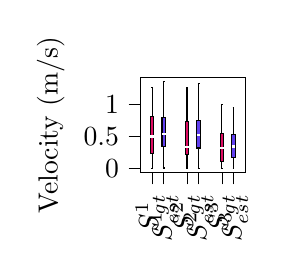
\begin{tikzpicture}

\definecolor{color0}{rgb}{0.870588235294118,0.0470588235294118,0.384313725490196}
\definecolor{color1}{rgb}{0.172549019607843,0.627450980392157,0.172549019607843}
\definecolor{color2}{rgb}{0.380392156862745,0.250980392156863,0.937254901960784}

\begin{axis}[
    width=\figurewidth,
    height=\figureheight,
tick align=outside,
tick pos=left,
x grid style={white!69.0196078431373!black},
xmin=0.5, xmax=5,
xtick style={color=black},
xtick={1,1.5,2.5,3,4,4.5},
xticklabel style={rotate=90},
xticklabels={$S^1_{gt}$,$S^1_{est}$,$S^2_{gt}$,$S^2_{est}$,$S^3_{gt}$,$S^3_{est}$},
y grid style={white!69.0196078431373!black},
ylabel={Velocity (m/s)},
ymin=-0.0675477474867174, ymax=1.41850269722107,
ytick style={color=black}
]
\path [draw=black, fill=color0]
(axis cs:0.925,0.228301763534546)
--(axis cs:1.075,0.228301763534546)
--(axis cs:1.075,0.803003311157227)
--(axis cs:0.925,0.803003311157227)
--(axis cs:0.925,0.228301763534546)
--cycle;
\addplot [black]
table {%
1 0.228301763534546
1 0
};
\addplot [black]
table {%
1 0.803003311157227
1 1.25467252731323
};
\addplot [black]
table {%
0.9625 0
1.0375 0
};
\addplot [black]
table {%
0.9625 1.25467252731323
1.0375 1.25467252731323
};
\path [draw=black, fill=color2]
(axis cs:1.425,0.345915478896163)
--(axis cs:1.575,0.345915478896163)
--(axis cs:1.575,0.795930253469308)
--(axis cs:1.425,0.795930253469308)
--(axis cs:1.425,0.345915478896163)
--cycle;
\addplot [black]
table {%
1.5 0.345915478896163
1.5 0.00287716614362132
};
\addplot [black]
table {%
1.5 0.795930253469308
1.5 1.35095494973435
};
\addplot [black]
table {%
1.4625 0.00287716614362132
1.5375 0.00287716614362132
};
\addplot [black]
table {%
1.4625 1.35095494973435
1.5375 1.35095494973435
};
\path [draw=black, fill=color0]
(axis cs:2.425,0.212566673755646)
--(axis cs:2.575,0.212566673755646)
--(axis cs:2.575,0.730346202850342)
--(axis cs:2.425,0.730346202850342)
--(axis cs:2.425,0.212566673755646)
--cycle;
\addplot [black]
table {%
2.5 0.212566673755646
2.5 0
};
\addplot [black]
table {%
2.5 0.730346202850342
2.5 1.25709009170532
};
\addplot [black]
table {%
2.4625 0
2.5375 0
};
\addplot [black]
table {%
2.4625 1.25709009170532
2.5375 1.25709009170532
};
\path [draw=black, fill=color2]
(axis cs:2.925,0.315225119374558)
--(axis cs:3.075,0.315225119374558)
--(axis cs:3.075,0.741941809976617)
--(axis cs:2.925,0.741941809976617)
--(axis cs:2.925,0.315225119374558)
--cycle;
\addplot [black]
table {%
3 0.315225119374558
3 0.00179093087536142
};
\addplot [black]
table {%
3 0.741941809976617
3 1.32119624163926
};
\addplot [black]
table {%
2.9625 0.00179093087536142
3.0375 0.00179093087536142
};
\addplot [black]
table {%
2.9625 1.32119624163926
3.0375 1.32119624163926
};
\path [draw=black, fill=color0]
(axis cs:3.925,0.0992751121520996)
--(axis cs:4.075,0.0992751121520996)
--(axis cs:4.075,0.545222759246826)
--(axis cs:3.925,0.545222759246826)
--(axis cs:3.925,0.0992751121520996)
--cycle;
\addplot [black]
table {%
4 0.0992751121520996
4 0
};
\addplot [black]
table {%
4 0.545222759246826
4 1.00019693374634
};
\addplot [black]
table {%
3.9625 0
4.0375 0
};
\addplot [black]
table {%
3.9625 1.00019693374634
4.0375 1.00019693374634
};
\path [draw=black, fill=color2]
(axis cs:4.425,0.160789500908161)
--(axis cs:4.575,0.160789500908161)
--(axis cs:4.575,0.530982102987396)
--(axis cs:4.425,0.530982102987396)
--(axis cs:4.425,0.160789500908161)
--cycle;
\addplot [black]
table {%
4.5 0.160789500908161
4.5 0.00151534690679966
};
\addplot [black]
table {%
4.5 0.530982102987396
4.5 0.94600199294792
};
\addplot [black]
table {%
4.4625 0.00151534690679966
4.5375 0.00151534690679966
};
\addplot [black]
table {%
4.4625 0.94600199294792
4.5375 0.94600199294792
};
\addplot [line width=1pt, white]
table {%
0.925 0.491624116897583
1.075 0.491624116897583
};
% \addplot [color1, mark=triangle*, mark size=3, mark options={solid}, only marks]
% table {%
% 1 0.596368908264476
% };
\addplot [line width=1pt, white]
table {%
1.425 0.533792302786217
1.575 0.533792302786217
};
% \addplot [color1, mark=triangle*, mark size=3, mark options={solid}, only marks]
% table {%
% 1.5 0.572308932232665
% };
\addplot [line width=1pt, white]
table {%
2.425 0.331982731819153
2.575 0.331982731819153
};
% \addplot [color1, mark=triangle*, mark size=3, mark options={solid}, only marks]
% table {%
% 2.5 0.464838665723801
% };
\addplot [line width=1pt, white]
table {%
2.925 0.517644409921193
3.075 0.517644409921193
};
% \addplot [color1, mark=triangle*, mark size=3, mark options={solid}, only marks]
% table {%
% 3 0.625595390180014
% };
\addplot [line width=1pt, white]
table {%
3.925 0.316886901855469
4.075 0.316886901855469
};
% \addplot [color1, mark=triangle*, mark size=3, mark options={solid}, only marks]
% table {%
% 4 0.357478909376191
% };
\addplot [line width=1pt, white]
table {%
4.425 0.338854789192458
4.575 0.338854789192458
};
% \addplot [color1, mark=triangle*, mark size=3, mark options={solid}, only marks]
% table {%
% 4.5 0.370969953522953
% };
\end{axis}

\end{tikzpicture}
}
%         \label{fig:Velo_x}
%         \caption{\scriptsize{Velo\_x}}
%     \end{subfigure}
%     \hfill
%     \begin{subfigure}{.23\textwidth}
%         \centering
%         \setlength{\figurewidth}{1.2\textwidth}
%         \setlength{\figureheight}{\textwidth}
%         \scriptsize{% This file was created with tikzplotlib v0.9.14.
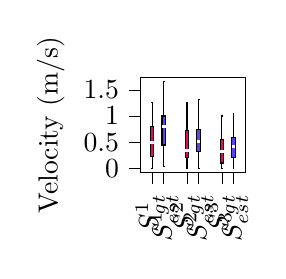
\begin{tikzpicture}

\definecolor{color0}{rgb}{0.870588235294118,0.0470588235294118,0.384313725490196}
\definecolor{color1}{rgb}{0.172549019607843,0.627450980392157,0.172549019607843}
\definecolor{color2}{rgb}{0.380392156862745,0.250980392156863,0.937254901960784}

\begin{axis}[
    width=\figurewidth,
    height=\figureheight,
tick align=outside,
tick pos=left,
x grid style={white!69.0196078431373!black},
xmin=0.5, xmax=5,
xtick style={color=black},
xtick={1,1.5,2.5,3,4,4.5},
xticklabel style={rotate=90},
xticklabels={$S^1_{gt}$,$S^1_{est}$,$S^2_{gt}$,$S^2_{est}$,$S^3_{gt}$,$S^3_{est}$},
% xticklabel style={rotate=45},
y grid style={white!69.0196078431373!black},
ylabel={Velocity (m/s)},
ymin=-0.0827635518386503, ymax=1.73803458861166,
ytick style={color=black}
]
\path [draw=black, fill=color0]
(axis cs:0.925,0.228301763534546)
--(axis cs:1.075,0.228301763534546)
--(axis cs:1.075,0.803003311157227)
--(axis cs:0.925,0.803003311157227)
--(axis cs:0.925,0.228301763534546)
--cycle;
\addplot [black]
table {%
1 0.228301763534546
1 0
};
\addplot [black]
table {%
1 0.803003311157227
1 1.25467252731323
};
\addplot [black]
table {%
0.9625 0
1.0375 0
};
\addplot [black]
table {%
0.9625 1.25467252731323
1.0375 1.25467252731323
};
\path [draw=black, fill=color2]
(axis cs:1.425,0.444815078086613)
--(axis cs:1.575,0.444815078086613)
--(axis cs:1.575,0.999803679059729)
--(axis cs:1.425,0.999803679059729)
--(axis cs:1.425,0.444815078086613)
--cycle;
\addplot [black]
table {%
1.5 0.444815078086613
1.5 0.0373116657325312
};
\addplot [black]
table {%
1.5 0.999803679059729
1.5 1.65527103677301
};
\addplot [black]
table {%
1.4625 0.0373116657325312
1.5375 0.0373116657325312
};
\addplot [black]
table {%
1.4625 1.65527103677301
1.5375 1.65527103677301
};
\path [draw=black, fill=color0]
(axis cs:2.425,0.212566673755646)
--(axis cs:2.575,0.212566673755646)
--(axis cs:2.575,0.730346202850342)
--(axis cs:2.425,0.730346202850342)
--(axis cs:2.425,0.212566673755646)
--cycle;
\addplot [black]
table {%
2.5 0.212566673755646
2.5 0
};
\addplot [black]
table {%
2.5 0.730346202850342
2.5 1.25709009170532
};
\addplot [black]
table {%
2.4625 0
2.5375 0
};
\addplot [black]
table {%
2.4625 1.25709009170532
2.5375 1.25709009170532
};
\path [draw=black, fill=color2]
(axis cs:2.925,0.315225119374558)
--(axis cs:3.075,0.315225119374558)
--(axis cs:3.075,0.741941809976617)
--(axis cs:2.925,0.741941809976617)
--(axis cs:2.925,0.315225119374558)
--cycle;
\addplot [black]
table {%
3 0.315225119374558
3 0.00179093087536142
};
\addplot [black]
table {%
3 0.741941809976617
3 1.32119624163926
};
\addplot [black]
table {%
2.9625 0.00179093087536142
3.0375 0.00179093087536142
};
\addplot [black]
table {%
2.9625 1.32119624163926
3.0375 1.32119624163926
};
\path [draw=black, fill=color0]
(axis cs:3.925,0.0992751121520996)
--(axis cs:4.075,0.0992751121520996)
--(axis cs:4.075,0.545222759246826)
--(axis cs:3.925,0.545222759246826)
--(axis cs:3.925,0.0992751121520996)
--cycle;
\addplot [black]
table {%
4 0.0992751121520996
4 0
};
\addplot [black]
table {%
4 0.545222759246826
4 1.00019693374634
};
\addplot [black]
table {%
3.9625 0
4.0375 0
};
\addplot [black]
table {%
3.9625 1.00019693374634
4.0375 1.00019693374634
};
\path [draw=black, fill=color2]
(axis cs:4.425,0.211098591176642)
--(axis cs:4.575,0.211098591176642)
--(axis cs:4.575,0.595357008744495)
--(axis cs:4.425,0.595357008744495)
--(axis cs:4.425,0.211098591176642)
--cycle;
\addplot [black]
table {%
4.5 0.211098591176642
4.5 0.00237383238998135
};
\addplot [black]
table {%
4.5 0.595357008744495
4.5 1.04749536722338
};
\addplot [black]
table {%
4.4625 0.00237383238998135
4.5375 0.00237383238998135
};
\addplot [black]
table {%
4.4625 1.04749536722338
4.5375 1.04749536722338
};
\addplot [line width=1pt, white]
table {%
0.925 0.491624116897583
1.075 0.491624116897583
};
% \addplot [color1, mark=triangle*, mark size=3, mark options={solid}, only marks]
% table {%
% 1 0.596368908264476
% };
\addplot [line width=1pt, white]
table {%
1.425 0.801675693519194
1.575 0.801675693519194
};
% \addplot [color1, mark=triangle*, mark size=3, mark options={solid}, only marks]
% table {%
% 1.5 0.765829195547974
% };
\addplot [line width=1pt, white]
table {%
2.425 0.331982731819153
2.575 0.331982731819153
};
% \addplot [color1, mark=triangle*, mark size=3, mark options={solid}, only marks]
% table {%
% 2.5 0.464838665723801
% };
\addplot [line width=1pt, white]
table {%
2.925 0.517644409921193
3.075 0.517644409921193
};
% \addplot [color1, mark=triangle*, mark size=3, mark options={solid}, only marks]
% table {%
% 3 0.625595390180014
% };
\addplot [line width=1pt, white]
table {%
3.925 0.316886901855469
4.075 0.316886901855469
};
% \addplot [color1, mark=triangle*, mark size=3, mark options={solid}, only marks]
% table {%
% 4 0.357478909376191
% };
\addplot [line width=1pt, white]
table {%
4.425 0.417277371600981
4.575 0.417277371600981
};
% \addplot [color1, mark=triangle*, mark size=3, mark options={solid}, only marks]
% table {%
% 4.5 0.41983885568837
% };
\end{axis}

\end{tikzpicture}
}
%         \caption{\scriptsize{Velo\_y}}
%         \label{fig:Velo_y}     
%     \end{subfigure}
%     \hfill
%     \begin{subfigure}{.23\textwidth}
%         \centering
%         \setlength{\figurewidth}{1.2\textwidth}
%         \setlength{\figureheight}{\textwidth}
%         \scriptsize{% This file was created with tikzplotlib v0.9.14.
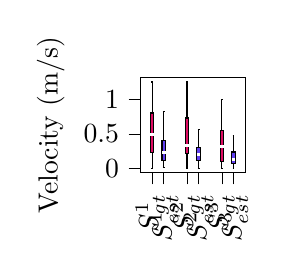
\begin{tikzpicture}

\definecolor{color0}{rgb}{0.870588235294118,0.0470588235294118,0.384313725490196}
\definecolor{color1}{rgb}{0.172549019607843,0.627450980392157,0.172549019607843}
\definecolor{color2}{rgb}{0.380392156862745,0.250980392156863,0.937254901960784}

\begin{axis}[
    width=\figurewidth,
    height=\figureheight,
tick align=outside,
tick pos=left,
x grid style={white!69.0196078431373!black},
xmin=0.5, xmax=5,
xtick style={color=black},
xtick={1,1.5,2.5,3,4,4.5},
xticklabel style={rotate=90},
xticklabels={$S^1_{gt}$,$S^1_{est}$,$S^2_{gt}$,$S^2_{est}$,$S^3_{gt}$,$S^3_{est}$},
y grid style={white!69.0196078431373!black},
ylabel={Velocity (m/s)},
ymin=-0.0628545045852661, ymax=1.31994459629059,
ytick style={color=black}
]
\path [draw=black, fill=color0]
(axis cs:0.925,0.228301763534546)
--(axis cs:1.075,0.228301763534546)
--(axis cs:1.075,0.803003311157227)
--(axis cs:0.925,0.803003311157227)
--(axis cs:0.925,0.228301763534546)
--cycle;
\addplot [black]
table {%
1 0.228301763534546
1 0
};
\addplot [black]
table {%
1 0.803003311157227
1 1.25467252731323
};
\addplot [black]
table {%
0.9625 0
1.0375 0
};
\addplot [black]
table {%
0.9625 1.25467252731323
1.0375 1.25467252731323
};
\path [draw=black, fill=color2]
(axis cs:1.425,0.113470833721045)
--(axis cs:1.575,0.113470833721045)
--(axis cs:1.575,0.398442972462949)
--(axis cs:1.425,0.398442972462949)
--(axis cs:1.425,0.113470833721045)
--cycle;
\addplot [black]
table {%
1.5 0.113470833721045
1.5 0.0105257916981311
};
\addplot [black]
table {%
1.5 0.398442972462949
1.5 0.821563747271634
};
\addplot [black]
table {%
1.4625 0.0105257916981311
1.5375 0.0105257916981311
};
\addplot [black]
table {%
1.4625 0.821563747271634
1.5375 0.821563747271634
};
\path [draw=black, fill=color0]
(axis cs:2.425,0.212566673755646)
--(axis cs:2.575,0.212566673755646)
--(axis cs:2.575,0.730346202850342)
--(axis cs:2.425,0.730346202850342)
--(axis cs:2.425,0.212566673755646)
--cycle;
\addplot [black]
table {%
2.5 0.212566673755646
2.5 0
};
\addplot [black]
table {%
2.5 0.730346202850342
2.5 1.25709009170532
};
\addplot [black]
table {%
2.4625 0
2.5375 0
};
\addplot [black]
table {%
2.4625 1.25709009170532
2.5375 1.25709009170532
};
\path [draw=black, fill=color2]
(axis cs:2.925,0.110751028617817)
--(axis cs:3.075,0.110751028617817)
--(axis cs:3.075,0.301799595829543)
--(axis cs:2.925,0.301799595829543)
--(axis cs:2.925,0.110751028617817)
--cycle;
\addplot [black]
table {%
3 0.110751028617817
3 0.000630204376011356
};
\addplot [black]
table {%
3 0.301799595829543
3 0.55998953885202
};
\addplot [black]
table {%
2.9625 0.000630204376011356
3.0375 0.000630204376011356
};
\addplot [black]
table {%
2.9625 0.55998953885202
3.0375 0.55998953885202
};
\path [draw=black, fill=color0]
(axis cs:3.925,0.0992751121520996)
--(axis cs:4.075,0.0992751121520996)
--(axis cs:4.075,0.545222759246826)
--(axis cs:3.925,0.545222759246826)
--(axis cs:3.925,0.0992751121520996)
--cycle;
\addplot [black]
table {%
4 0.0992751121520996
4 0
};
\addplot [black]
table {%
4 0.545222759246826
4 1.00019693374634
};
\addplot [black]
table {%
3.9625 0
4.0375 0
};
\addplot [black]
table {%
3.9625 1.00019693374634
4.0375 1.00019693374634
};
\path [draw=black, fill=color2]
(axis cs:4.425,0.0645805682441358)
--(axis cs:4.575,0.0645805682441358)
--(axis cs:4.575,0.235053128543875)
--(axis cs:4.425,0.235053128543875)
--(axis cs:4.425,0.0645805682441358)
--cycle;
\addplot [black]
table {%
4.5 0.0645805682441358
4.5 0.000576203866032854
};
\addplot [black]
table {%
4.5 0.235053128543875
4.5 0.47113530926346
};
\addplot [black]
table {%
4.4625 0.000576203866032854
4.5375 0.000576203866032854
};
\addplot [black]
table {%
4.4625 0.47113530926346
4.5375 0.47113530926346
};
\addplot [line width=1pt, white]
table {%
0.925 0.491624116897583
1.075 0.491624116897583
};
% \addplot [color1, mark=triangle*, mark size=3, mark options={solid}, only marks]
% table {%
% 1 0.596368908264476
% };
\addplot [line width=1pt, white]
table {%
1.425 0.232014217104268
1.575 0.232014217104268
};
% \addplot [color1, mark=triangle*, mark size=3, mark options={solid}, only marks]
% table {%
% 1.5 0.295426155215103
% };
\addplot [line width=1pt, white]
table {%
2.425 0.331982731819153
2.575 0.331982731819153
};
% \addplot [color1, mark=triangle*, mark size=3, mark options={solid}, only marks]
% table {%
% 2.5 0.464838665723801
% };
\addplot [line width=1pt, white]
table {%
2.925 0.201312865262763
3.075 0.201312865262763
};
% \addplot [color1, mark=triangle*, mark size=3, mark options={solid}, only marks]
% table {%
% 3 0.255979156305825
% };
\addplot [line width=1pt, white]
table {%
3.925 0.316886901855469
4.075 0.316886901855469
};
% \addplot [color1, mark=triangle*, mark size=3, mark options={solid}, only marks]
% table {%
% 4 0.357478909376191
% };
\addplot [line width=1pt, white]
table {%
4.425 0.127364749837743
4.575 0.127364749837743
};
% \addplot [color1, mark=triangle*, mark size=3, mark options={solid}, only marks]
% table {%
% 4.5 0.166514199058239
% };
\end{axis}

\end{tikzpicture}
}
%         \caption{\scriptsize{Velo\_y}}
%         \label{fig:Velo_y}     
%     \end{subfigure}
%     \hfill
%     \begin{subfigure}{.23\textwidth}
%         \centering
%         \setlength{\figurewidth}{1.2\textwidth}
%         \setlength{\figureheight}{\textwidth}
%         \scriptsize{% This file was created with tikzplotlib v0.9.14.
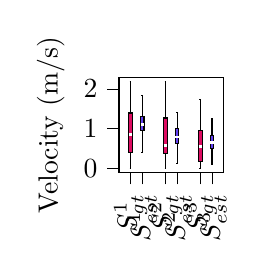
\begin{tikzpicture}

\definecolor{color0}{rgb}{0.870588235294118,0.0470588235294118,0.384313725490196}
\definecolor{color1}{rgb}{0.172549019607843,0.627450980392157,0.172549019607843}
\definecolor{color2}{rgb}{0.380392156862745,0.250980392156863,0.937254901960784}

\begin{axis}[
    width=\figurewidth,
    height=\figureheight,
tick align=outside,
tick pos=left,
x grid style={white!69.0196078431373!black},
xmin=0.5, xmax=5,
xtick style={color=black},
xtick={1,1.5,2.5,3,4,4.5},
xticklabel style={rotate=90},
xticklabels={$S^1_{gt}$,$S^1_{est}$,$S^2_{gt}$,$S^2_{est}$,$S^3_{gt}$,$S^3_{est}$},
y grid style={white!69.0196078431373!black},
ylabel={Velocity (m/s)},
ymin=-0.108867195426252, ymax=2.28621110395129,
ytick style={color=black}
]
\path [draw=black, fill=color0]
(axis cs:0.925,0.395430253899409)
--(axis cs:1.075,0.395430253899409)
--(axis cs:1.075,1.39084253357036)
--(axis cs:0.925,1.39084253357036)
--(axis cs:0.925,0.395430253899409)
--cycle;
\addplot [black]
table {%
1 0.395430253899409
1 0
};
\addplot [black]
table {%
1 1.39084253357036
1 2.17315656416737
};
\addplot [black]
table {%
0.9625 0
1.0375 0
};
\addplot [black]
table {%
0.9625 2.17315656416737
1.0375 2.17315656416737
};
\path [draw=black, fill=color2]
(axis cs:1.425,0.941181742088769)
--(axis cs:1.575,0.941181742088769)
--(axis cs:1.575,1.30615450665097)
--(axis cs:1.425,1.30615450665097)
--(axis cs:1.425,0.941181742088769)
--cycle;
\addplot [black]
table {%
1.5 0.941181742088769
1.5 0.400352838078203
};
\addplot [black]
table {%
1.5 1.30615450665097
1.5 1.83474493679979
};
\addplot [black]
table {%
1.4625 0.400352838078203
1.5375 0.400352838078203
};
\addplot [black]
table {%
1.4625 1.83474493679979
1.5375 1.83474493679979
};
\path [draw=black, fill=color0]
(axis cs:2.425,0.368176278940696)
--(axis cs:2.575,0.368176278940696)
--(axis cs:2.575,1.2649967304518)
--(axis cs:2.425,1.2649967304518)
--(axis cs:2.425,0.368176278940696)
--cycle;
\addplot [black]
table {%
2.5 0.368176278940696
2.5 0
};
\addplot [black]
table {%
2.5 1.2649967304518
2.5 2.17734390852504
};
\addplot [black]
table {%
2.4625 0
2.5375 0
};
\addplot [black]
table {%
2.4625 2.17734390852504
2.5375 2.17734390852504
};
\path [draw=black, fill=color2]
(axis cs:2.925,0.620111065408091)
--(axis cs:3.075,0.620111065408091)
--(axis cs:3.075,0.992183801791019)
--(axis cs:2.925,0.992183801791019)
--(axis cs:2.925,0.620111065408091)
--cycle;
\addplot [black]
table {%
3 0.620111065408091
3 0.113923421243718
};
\addplot [black]
table {%
3 0.992183801791019
3 1.3950839521451
};
\addplot [black]
table {%
2.9625 0.113923421243718
3.0375 0.113923421243718
};
\addplot [black]
table {%
2.9625 1.3950839521451
3.0375 1.3950839521451
};
\path [draw=black, fill=color0]
(axis cs:3.925,0.171949538174535)
--(axis cs:4.075,0.171949538174535)
--(axis cs:4.075,0.944353520458397)
--(axis cs:3.925,0.944353520458397)
--(axis cs:3.925,0.171949538174535)
--cycle;
\addplot [black]
table {%
4 0.171949538174535
4 0
};
\addplot [black]
table {%
4 0.944353520458397
4 1.73239190682326
};
\addplot [black]
table {%
3.9625 0
4.0375 0
};
\addplot [black]
table {%
3.9625 1.73239190682326
4.0375 1.73239190682326
};
\path [draw=black, fill=color2]
(axis cs:4.425,0.496256182549431)
--(axis cs:4.575,0.496256182549431)
--(axis cs:4.575,0.82581732680424)
--(axis cs:4.425,0.82581732680424)
--(axis cs:4.425,0.496256182549431)
--cycle;
\addplot [black]
table {%
4.5 0.496256182549431
4.5 0.0876241192954267
};
\addplot [black]
table {%
4.5 0.82581732680424
4.5 1.2516592273785
};
\addplot [black]
table {%
4.4625 0.0876241192954267
4.5375 0.0876241192954267
};
\addplot [black]
table {%
4.4625 1.2516592273785
4.5375 1.2516592273785
};
\addplot [line width=1pt, white]
table {%
0.925 0.851517948692795
1.075 0.851517948692795
};
% \addplot [color1, mark=triangle*, mark size=3, mark options={solid}, only marks]
% table {%
% 1 1.03294124916846
% };
\addplot [line width=1pt, white]
table {%
1.425 1.09400778779152
1.575 1.09400778779152
};
% \addplot [color1, mark=triangle*, mark size=3, mark options={solid}, only marks]
% table {%
% 1.5 1.11454884167741
% };
\addplot [line width=1pt, white]
table {%
2.425 0.575010958746286
2.575 0.575010958746286
};
% \addplot [color1, mark=triangle*, mark size=3, mark options={solid}, only marks]
% table {%
% 2.5 0.805124186356148
% };
\addplot [line width=1pt, white]
table {%
2.925 0.785511883398785
3.075 0.785511883398785
};
% \addplot [color1, mark=triangle*, mark size=3, mark options={solid}, only marks]
% table {%
% 3 0.891858915137335
% };
\addplot [line width=1pt, white]
table {%
3.925 0.548864214266764
4.075 0.548864214266764
};
% \addplot [color1, mark=triangle*, mark size=3, mark options={solid}, only marks]
% table {%
% 4 0.619171633673873
% };
\addplot [line width=1pt, white]
table {%
4.425 0.6431148242745
4.575 0.6431148242745
};
% \addplot [color1, mark=triangle*, mark size=3, mark options={solid}, only marks]
% table {%
% 4.5 0.652855139469089
% };
\end{axis}

\end{tikzpicture}
}
%         \caption{\scriptsize{Velo\_all}}
%         \label{fig:Velo_y}     
%     \end{subfigure}
%     \caption{On the left is a top view of the trajectory comparison, and on the right is a side view of the trajectory comparison.}
%     \label{fig:velo_xyza}
% \end{figure*}



% \subsection{blah blah}
% We also compared our method with a UAV tracking method based on Ouster OS0-128 LiDAR images and point clouds in the environment of \textit{Seq 3}, and the trajectories are shown in Fig~\ref{fig:full_traj}. The point cloud tracking method only uses Ouster OS0-128 LiDAR point cloud data as input, with a frame rate of 10Hz. When tracking the UAV using only point cloud data as input, we need to know the initial position of the UAV, because the point cloud of the UAV is sparser than that of larger objects such as cars or humans, and it is difficult to distinguish the point cloud of the UAV from the environment using features. The image tracking method only uses Ouster OS0-128 LiDAR signal images, with a frame rate of 10Hz. First, the signal image is subjected to target detection processing to obtain the bounding box of the UAV in the signal image, and then the image in the bounding box is converted into point cloud data. After obtaining the point cloud in the ROI, the point cloud clustering algorithm is used to separate the point cloud of the UAV based on the number and distance features of the point cloud clusters, thus obtaining the trajectory of the UAV.
% \begin{figure}[htb] 
%     \centering   
%     \includegraphics[width=0.4\textwidth]{fig/to_do_sign.png}  
%     \caption{traj-fig to fill.}
%     \label{fig:to-do} 
% \end{figure}
% \begin{figure}[h] 
%     \centering 
%     \scriptsize{% This file was created with tikzplotlib v0.9.14.
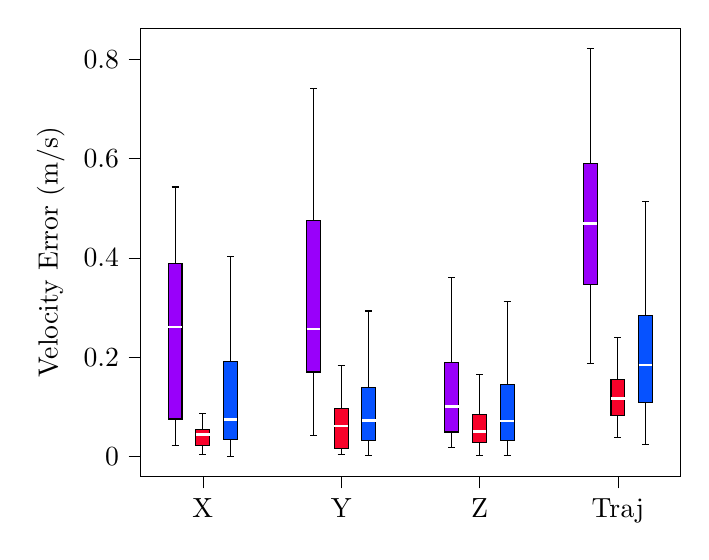
\begin{tikzpicture}

\definecolor{color0}{rgb}{0.6,0,0.980392156862745}
\definecolor{color1}{rgb}{0.968627450980392,0.00784313725490196,0.164705882352941}
\definecolor{color2}{rgb}{0.0235294117647059,0.32156862745098,1}

\begin{axis}[
legend cell align={left},
legend style={
  fill opacity=0.8,
  draw opacity=1,
  text opacity=1,
  at={(0.03,0.97)},
  anchor=north west,
  draw=white!80!black
},
tick align=outside,
tick pos=left,
x grid style={white!69.0196078431373!black},
xmin=0.5, xmax=8.3,
xtick style={color=black},
xtick={1.4,3.4,5.4,7.4},
xticklabels={X,Y,Z,Traj},
y grid style={white!69.0196078431373!black},
ylabel={Velocity Error (m/s)},
ymin=-0.0403882278249122, ymax=0.862144572706216,
ytick style={color=black}
]
\path [draw=black, fill=color0]
(axis cs:0.9,0.075331025851198)
--(axis cs:1.1,0.075331025851198)
--(axis cs:1.1,0.388781930340623)
--(axis cs:0.9,0.388781930340623)
--(axis cs:0.9,0.075331025851198)
--cycle;
\addplot [black, forget plot]
table {%
1 0.075331025851198
1 0.0223148850774031
};
\addplot [black, forget plot]
table {%
1 0.388781930340623
1 0.542564255496907
};
\addplot [black, forget plot]
table {%
0.95 0.0223148850774031
1.05 0.0223148850774031
};
\addplot [black, forget plot]
table {%
0.95 0.542564255496907
1.05 0.542564255496907
};
\path [draw=black, fill=color1]
(axis cs:1.3,0.0217070569597944)
--(axis cs:1.5,0.0217070569597944)
--(axis cs:1.5,0.0546994247647747)
--(axis cs:1.3,0.0546994247647747)
--(axis cs:1.3,0.0217070569597944)
--cycle;
\addplot [black, forget plot]
table {%
1.4 0.0217070569597944
1.4 0.00352621215375493
};
\addplot [black, forget plot]
table {%
1.4 0.0546994247647747
1.4 0.0865244006083676
};
\addplot [black, forget plot]
table {%
1.35 0.00352621215375493
1.45 0.00352621215375493
};
\addplot [black, forget plot]
table {%
1.35 0.0865244006083676
1.45 0.0865244006083676
};
\path [draw=black, fill=color2]
(axis cs:1.7,0.0332886140400268)
--(axis cs:1.9,0.0332886140400268)
--(axis cs:1.9,0.19141703059926)
--(axis cs:1.7,0.19141703059926)
--(axis cs:1.7,0.0332886140400268)
--cycle;
\addplot [black, forget plot]
table {%
1.8 0.0332886140400268
1.8 0.000635990381048224
};
\addplot [black, forget plot]
table {%
1.8 0.19141703059926
1.8 0.402100357756092
};
\addplot [black, forget plot]
table {%
1.75 0.000635990381048224
1.85 0.000635990381048224
};
\addplot [black, forget plot]
table {%
1.75 0.402100357756092
1.85 0.402100357756092
};
\path [draw=black, fill=color0]
(axis cs:2.9,0.169990197655884)
--(axis cs:3.1,0.169990197655884)
--(axis cs:3.1,0.475912431655918)
--(axis cs:2.9,0.475912431655918)
--(axis cs:2.9,0.169990197655884)
--cycle;
\addplot [black, forget plot]
table {%
3 0.169990197655884
3 0.042828844665673
};
\addplot [black, forget plot]
table {%
3 0.475912431655918
3 0.740511941235374
};
\addplot [black, forget plot]
table {%
2.95 0.042828844665673
3.05 0.042828844665673
};
\addplot [black, forget plot]
table {%
2.95 0.740511941235374
3.05 0.740511941235374
};
\path [draw=black, fill=color1]
(axis cs:3.3,0.0157473096754768)
--(axis cs:3.5,0.0157473096754768)
--(axis cs:3.5,0.0958901340197926)
--(axis cs:3.3,0.0958901340197926)
--(axis cs:3.3,0.0157473096754768)
--cycle;
\addplot [black, forget plot]
table {%
3.4 0.0157473096754768
3.4 0.00351959530062285
};
\addplot [black, forget plot]
table {%
3.4 0.0958901340197926
3.4 0.183003675718196
};
\addplot [black, forget plot]
table {%
3.35 0.00351959530062285
3.45 0.00351959530062285
};
\addplot [black, forget plot]
table {%
3.35 0.183003675718196
3.45 0.183003675718196
};
\path [draw=black, fill=color2]
(axis cs:3.7,0.0315928666809684)
--(axis cs:3.9,0.0315928666809684)
--(axis cs:3.9,0.138337363062844)
--(axis cs:3.7,0.138337363062844)
--(axis cs:3.7,0.0315928666809684)
--cycle;
\addplot [black, forget plot]
table {%
3.8 0.0315928666809684
3.8 0.00131056242322458
};
\addplot [black, forget plot]
table {%
3.8 0.138337363062844
3.8 0.292953311866837
};
\addplot [black, forget plot]
table {%
3.75 0.00131056242322458
3.85 0.00131056242322458
};
\addplot [black, forget plot]
table {%
3.75 0.292953311866837
3.85 0.292953311866837
};
\path [draw=black, fill=color0]
(axis cs:4.9,0.0491585177890972)
--(axis cs:5.1,0.0491585177890972)
--(axis cs:5.1,0.189313611734313)
--(axis cs:4.9,0.189313611734313)
--(axis cs:4.9,0.0491585177890972)
--cycle;
\addplot [black, forget plot]
table {%
5 0.0491585177890972
5 0.0179027446331044
};
\addplot [black, forget plot]
table {%
5 0.189313611734313
5 0.36036437044022
};
\addplot [black, forget plot]
table {%
4.95 0.0179027446331044
5.05 0.0179027446331044
};
\addplot [black, forget plot]
table {%
4.95 0.36036437044022
5.05 0.36036437044022
};
\path [draw=black, fill=color1]
(axis cs:5.3,0.0283181876034852)
--(axis cs:5.5,0.0283181876034852)
--(axis cs:5.5,0.0841908035928116)
--(axis cs:5.3,0.0841908035928116)
--(axis cs:5.3,0.0283181876034852)
--cycle;
\addplot [black, forget plot]
table {%
5.4 0.0283181876034852
5.4 0.00137162626933862
};
\addplot [black, forget plot]
table {%
5.4 0.0841908035928116
5.4 0.164295546110094
};
\addplot [black, forget plot]
table {%
5.35 0.00137162626933862
5.45 0.00137162626933862
};
\addplot [black, forget plot]
table {%
5.35 0.164295546110094
5.45 0.164295546110094
};
\path [draw=black, fill=color2]
(axis cs:5.7,0.0315878910472867)
--(axis cs:5.9,0.0315878910472867)
--(axis cs:5.9,0.144246711391837)
--(axis cs:5.7,0.144246711391837)
--(axis cs:5.7,0.0315878910472867)
--cycle;
\addplot [black, forget plot]
table {%
5.8 0.0315878910472867
5.8 0.00268274559533599
};
\addplot [black, forget plot]
table {%
5.8 0.144246711391837
5.8 0.311185092802099
};
\addplot [black, forget plot]
table {%
5.75 0.00268274559533599
5.85 0.00268274559533599
};
\addplot [black, forget plot]
table {%
5.75 0.311185092802099
5.85 0.311185092802099
};
\path [draw=black, fill=color0]
(axis cs:6.9,0.3459828068099)
--(axis cs:7.1,0.3459828068099)
--(axis cs:7.1,0.590554533840883)
--(axis cs:6.9,0.590554533840883)
--(axis cs:6.9,0.3459828068099)
--cycle;
\addplot [black, forget plot]
table {%
7 0.3459828068099
7 0.186642545736422
};
\addplot [black, forget plot]
table {%
7 0.590554533840883
7 0.821120354500256
};
\addplot [black, forget plot]
table {%
6.95 0.186642545736422
7.05 0.186642545736422
};
\addplot [black, forget plot]
table {%
6.95 0.821120354500256
7.05 0.821120354500256
};
\path [draw=black, fill=color1]
(axis cs:7.3,0.0820777035987898)
--(axis cs:7.5,0.0820777035987898)
--(axis cs:7.5,0.155043841711235)
--(axis cs:7.3,0.155043841711235)
--(axis cs:7.3,0.0820777035987898)
--cycle;
\addplot [black, forget plot]
table {%
7.4 0.0820777035987898
7.4 0.038816234445421
};
\addplot [black, forget plot]
table {%
7.4 0.155043841711235
7.4 0.238862504550516
};
\addplot [black, forget plot]
table {%
7.35 0.038816234445421
7.45 0.038816234445421
};
\addplot [black, forget plot]
table {%
7.35 0.238862504550516
7.45 0.238862504550516
};
\path [draw=black, fill=color2]
(axis cs:7.7,0.108502081919612)
--(axis cs:7.9,0.108502081919612)
--(axis cs:7.9,0.284651138459915)
--(axis cs:7.7,0.284651138459915)
--(axis cs:7.7,0.108502081919612)
--cycle;
\addplot [black, forget plot]
table {%
7.8 0.108502081919612
7.8 0.024657186551901
};
\addplot [black, forget plot]
table {%
7.8 0.284651138459915
7.8 0.512915034364593
};
\addplot [black, forget plot]
table {%
7.75 0.024657186551901
7.85 0.024657186551901
};
\addplot [black, forget plot]
table {%
7.75 0.512915034364593
7.85 0.512915034364593
};
\addplot [line width=1pt, white, forget plot]
table {%
0.9 0.260803583949127
1.1 0.260803583949127
};
\addplot [line width=1pt, white, forget plot]
table {%
1.3 0.0438217532799601
1.5 0.0438217532799601
};
\addplot [line width=1pt, white, forget plot]
table {%
1.7 0.0739501251040564
1.9 0.0739501251040564
};
\addplot [line width=1pt, white, forget plot]
table {%
2.9 0.256659941040683
3.1 0.256659941040683
};
\addplot [line width=1pt, white, forget plot]
table {%
3.3 0.061504939272532
3.5 0.061504939272532
};
\addplot [line width=1pt, white, forget plot]
table {%
3.7 0.0727679202697828
3.9 0.0727679202697828
};
\addplot [line width=1pt, white, forget plot]
table {%
4.9 0.100280910532975
5.1 0.100280910532975
};
\addplot [line width=1pt, white, forget plot]
table {%
5.3 0.0498791556970923
5.5 0.0498791556970923
};
\addplot [line width=1pt, white, forget plot]
table {%
5.7 0.0715585282181058
5.9 0.0715585282181058
};
\addplot [line width=1pt, white, forget plot]
table {%
6.9 0.469156620244255
7.1 0.469156620244255
};
\addplot [line width=1pt, white, forget plot]
table {%
7.3 0.11608448207449
7.5 0.11608448207449
};
\addplot [line width=1pt, white, forget plot]
table {%
7.7 0.184174965298658
7.9 0.184174965298658
};
\end{axis}

\end{tikzpicture}
}
%     \caption{compare velo error of different methods. }
%     \label{fig:velo_arr} 
% \end{figure}


% Table~\ref{tab:methods_compare} compares these three methods in terms of detectable range, average ATE error and root mean square error (RMSE), operating speed, and prerequisite conditions, while Fig~\ref{fig:vel_errs} shows the velocity error of different UAV tracking methods.
% Based on the experimental results above, it can be concluded that the point cloud tracking method is superior to the image tracking method in terms of the detectable range, but the method runs slowly, with an average frame rate of only 1.55 Hz, because this method does not limit the number of point clouds to be clustered by selecting ROI. Moreover, due to the slow running speed, the speed error of this method is very large.Although the image tracking method has advantages in accuracy and operating speed, and the speed error of this method is the smallest, the detection distance of this method is only 2.4 m. Our method combines Ouster OS0-128 LiDAR image and point cloud data, which has advantages in both running speed and detection range. Although the error is slightly larger than that of the image tracking method, the average error is only 3.6 cm, and the speed error is not significantly different from that of the image tracking method, only slightly larger, with a total error of about 0.19 m/s.












% \begin{figure}[htb] 
%     \centering   
%     \includegraphics[width=0.45\textwidth]{fig/box_error.png}  
%     \caption{Box plot of the error of X value, Y value, Z value, and trajectory (Euclidean distance). }
%     \label{fig:box_error} 
% \end{figure}

% \begin{figure}[t] 
%     \centering 
%     \scriptsize{% This file was created with tikzplotlib v0.9.14.
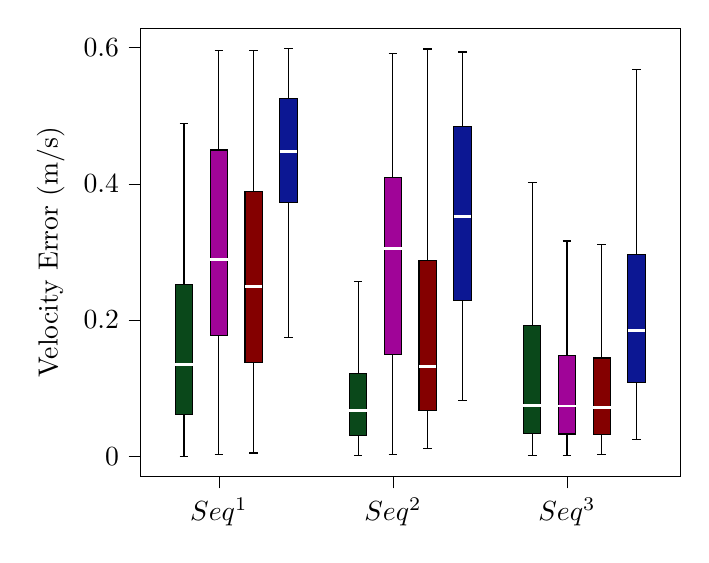
\begin{tikzpicture}

\definecolor{color0}{rgb}{0.0392156862745098,0.282352941176471,0.101960784313725}
\definecolor{color1}{rgb}{0.627450980392157,0.0156862745098039,0.596078431372549}
\definecolor{color2}{rgb}{0.0470588235294118,0.0901960784313725,0.576470588235294}

\begin{axis}[
legend cell align={left},
legend style={
  fill opacity=0.8,
  draw opacity=1,
  text opacity=1,
  at={(0.03,0.97)},
  anchor=north west,
  draw=white!80!black
},
tick align=outside,
tick pos=left,
x grid style={white!69.0196078431373!black},
xmin=0.5, xmax=6.7,
xtick style={color=black},
xtick={1.4,3.4,5.4},
xticklabels={$Seq^1$,$Seq^2$,$Seq^3$},
y grid style={white!69.0196078431373!black},
ylabel={Velocity Error (m/s)},
ymin=-0.0298483261699612, ymax=0.628427089758528,
ytick style={color=black}
]
\path [draw=black, fill=color0]
(axis cs:0.9,0.0610462777542375)
--(axis cs:1.1,0.0610462777542375)
--(axis cs:1.1,0.251716065963832)
--(axis cs:0.9,0.251716065963832)
--(axis cs:0.9,0.0610462777542375)
--cycle;
\addplot [black, forget plot]
table {%
1 0.0610462777542375
1 7.32836449701679e-05
};
\addplot [black, forget plot]
table {%
1 0.251716065963832
1 0.488183398388942
};
\addplot [black, forget plot]
table {%
0.95 7.32836449701679e-05
1.05 7.32836449701679e-05
};
\addplot [black, forget plot]
table {%
0.95 0.488183398388942
1.05 0.488183398388942
};
\path [draw=black, fill=color1]
(axis cs:1.3,0.177610035147419)
--(axis cs:1.5,0.177610035147419)
--(axis cs:1.5,0.449675727250805)
--(axis cs:1.3,0.449675727250805)
--(axis cs:1.3,0.177610035147419)
--cycle;
\addplot [black, forget plot]
table {%
1.4 0.177610035147419
1.4 0.0023949624187658
};
\addplot [black, forget plot]
table {%
1.4 0.449675727250805
1.4 0.595338376221308
};
\addplot [black, forget plot]
table {%
1.35 0.0023949624187658
1.45 0.0023949624187658
};
\addplot [black, forget plot]
table {%
1.35 0.595338376221308
1.45 0.595338376221308
};
\path [draw=black, fill=red!51.7647058823529!black]
(axis cs:1.7,0.137953780734275)
--(axis cs:1.9,0.137953780734275)
--(axis cs:1.9,0.388440654417876)
--(axis cs:1.7,0.388440654417876)
--(axis cs:1.7,0.137953780734275)
--cycle;
\addplot [black, forget plot]
table {%
1.8 0.137953780734275
1.8 0.00473007136044701
};
\addplot [black, forget plot]
table {%
1.8 0.388440654417876
1.8 0.595076896115714
};
\addplot [black, forget plot]
table {%
1.75 0.00473007136044701
1.85 0.00473007136044701
};
\addplot [black, forget plot]
table {%
1.75 0.595076896115714
1.85 0.595076896115714
};
\path [draw=black, fill=color2]
(axis cs:2.1,0.372285519453117)
--(axis cs:2.3,0.372285519453117)
--(axis cs:2.3,0.524950572995953)
--(axis cs:2.1,0.524950572995953)
--(axis cs:2.1,0.372285519453117)
--cycle;
\addplot [black, forget plot]
table {%
2.2 0.372285519453117
2.2 0.174768843643038
};
\addplot [black, forget plot]
table {%
2.2 0.524950572995953
2.2 0.598505479943596
};
\addplot [black, forget plot]
table {%
2.15 0.174768843643038
2.25 0.174768843643038
};
\addplot [black, forget plot]
table {%
2.15 0.598505479943596
2.25 0.598505479943596
};
\path [draw=black, fill=color0]
(axis cs:2.9,0.0310470276541031)
--(axis cs:3.1,0.0310470276541031)
--(axis cs:3.1,0.12176457855323)
--(axis cs:2.9,0.12176457855323)
--(axis cs:2.9,0.0310470276541031)
--cycle;
\addplot [black, forget plot]
table {%
3 0.0310470276541031
3 0.00155012128587817
};
\addplot [black, forget plot]
table {%
3 0.12176457855323
3 0.256631309238178
};
\addplot [black, forget plot]
table {%
2.95 0.00155012128587817
3.05 0.00155012128587817
};
\addplot [black, forget plot]
table {%
2.95 0.256631309238178
3.05 0.256631309238178
};
\path [draw=black, fill=color1]
(axis cs:3.3,0.148977968583482)
--(axis cs:3.5,0.148977968583482)
--(axis cs:3.5,0.408763744813898)
--(axis cs:3.3,0.408763744813898)
--(axis cs:3.3,0.148977968583482)
--cycle;
\addplot [black, forget plot]
table {%
3.4 0.148977968583482
3.4 0.00250996215517496
};
\addplot [black, forget plot]
table {%
3.4 0.408763744813898
3.4 0.591429347259549
};
\addplot [black, forget plot]
table {%
3.35 0.00250996215517496
3.45 0.00250996215517496
};
\addplot [black, forget plot]
table {%
3.35 0.591429347259549
3.45 0.591429347259549
};
\path [draw=black, fill=red!51.7647058823529!black]
(axis cs:3.7,0.0674717168155389)
--(axis cs:3.9,0.0674717168155389)
--(axis cs:3.9,0.28783706080661)
--(axis cs:3.7,0.28783706080661)
--(axis cs:3.7,0.0674717168155389)
--cycle;
\addplot [black, forget plot]
table {%
3.8 0.0674717168155389
3.8 0.0114388920134345
};
\addplot [black, forget plot]
table {%
3.8 0.28783706080661
3.8 0.597991973978502
};
\addplot [black, forget plot]
table {%
3.75 0.0114388920134345
3.85 0.0114388920134345
};
\addplot [black, forget plot]
table {%
3.75 0.597991973978502
3.85 0.597991973978502
};
\path [draw=black, fill=color2]
(axis cs:4.1,0.228594804047771)
--(axis cs:4.3,0.228594804047771)
--(axis cs:4.3,0.483983635249305)
--(axis cs:4.1,0.483983635249305)
--(axis cs:4.1,0.228594804047771)
--cycle;
\addplot [black, forget plot]
table {%
4.2 0.228594804047771
4.2 0.0813244583746304
};
\addplot [black, forget plot]
table {%
4.2 0.483983635249305
4.2 0.593453650512267
};
\addplot [black, forget plot]
table {%
4.15 0.0813244583746304
4.25 0.0813244583746304
};
\addplot [black, forget plot]
table {%
4.15 0.593453650512267
4.25 0.593453650512267
};
\path [draw=black, fill=color0]
(axis cs:4.9,0.0332886140400268)
--(axis cs:5.1,0.0332886140400268)
--(axis cs:5.1,0.19141703059926)
--(axis cs:4.9,0.19141703059926)
--(axis cs:4.9,0.0332886140400268)
--cycle;
\addplot [black, forget plot]
table {%
5 0.0332886140400268
5 0.000635990381048224
};
\addplot [black, forget plot]
table {%
5 0.19141703059926
5 0.402100357756092
};
\addplot [black, forget plot]
table {%
4.95 0.000635990381048224
5.05 0.000635990381048224
};
\addplot [black, forget plot]
table {%
4.95 0.402100357756092
5.05 0.402100357756092
};
\path [draw=black, fill=color1]
(axis cs:5.3,0.0326411668857862)
--(axis cs:5.5,0.0326411668857862)
--(axis cs:5.5,0.148022968453305)
--(axis cs:5.3,0.148022968453305)
--(axis cs:5.3,0.0326411668857862)
--cycle;
\addplot [black, forget plot]
table {%
5.4 0.0326411668857862
5.4 0.00131056242322458
};
\addplot [black, forget plot]
table {%
5.4 0.148022968453305
5.4 0.315998510977415
};
\addplot [black, forget plot]
table {%
5.35 0.00131056242322458
5.45 0.00131056242322458
};
\addplot [black, forget plot]
table {%
5.35 0.315998510977415
5.45 0.315998510977415
};
\path [draw=black, fill=red!51.7647058823529!black]
(axis cs:5.7,0.0315878910472867)
--(axis cs:5.9,0.0315878910472867)
--(axis cs:5.9,0.144246711391837)
--(axis cs:5.7,0.144246711391837)
--(axis cs:5.7,0.0315878910472867)
--cycle;
\addplot [black, forget plot]
table {%
5.8 0.0315878910472867
5.8 0.00268274559533599
};
\addplot [black, forget plot]
table {%
5.8 0.144246711391837
5.8 0.311185092802099
};
\addplot [black, forget plot]
table {%
5.75 0.00268274559533599
5.85 0.00268274559533599
};
\addplot [black, forget plot]
table {%
5.75 0.311185092802099
5.85 0.311185092802099
};
\path [draw=black, fill=color2]
(axis cs:6.1,0.10859210618893)
--(axis cs:6.3,0.10859210618893)
--(axis cs:6.3,0.296439930951403)
--(axis cs:6.1,0.296439930951403)
--(axis cs:6.1,0.10859210618893)
--cycle;
\addplot [black, forget plot]
table {%
6.2 0.10859210618893
6.2 0.024657186551901
};
\addplot [black, forget plot]
table {%
6.2 0.296439930951403
6.2 0.567549807740381
};
\addplot [black, forget plot]
table {%
6.15 0.024657186551901
6.25 0.024657186551901
};
\addplot [black, forget plot]
table {%
6.15 0.567549807740381
6.25 0.567549807740381
};
\addplot [line width=1pt, white, forget plot]
table {%
0.9 0.134893165702126
1.1 0.134893165702126
};
\addplot [line width=1pt, white, forget plot]
table {%
1.3 0.28923681918398
1.5 0.28923681918398
};
\addplot [line width=1pt, white, forget plot]
table {%
1.7 0.248659865769282
1.9 0.248659865769282
};
\addplot [line width=1pt, white, forget plot]
table {%
2.1 0.447386340670933
2.3 0.447386340670933
};
\addplot [line width=1pt, white, forget plot]
table {%
2.9 0.0667883769203348
3.1 0.0667883769203348
};
\addplot [line width=1pt, white, forget plot]
table {%
3.3 0.304836412692187
3.5 0.304836412692187
};
\addplot [line width=1pt, white, forget plot]
table {%
3.7 0.131350867943023
3.9 0.131350867943023
};
\addplot [line width=1pt, white, forget plot]
table {%
4.1 0.352492654874463
4.3 0.352492654874463
};
\addplot [line width=1pt, white, forget plot]
table {%
4.9 0.0739501251040564
5.1 0.0739501251040564
};
\addplot [line width=1pt, white, forget plot]
table {%
5.3 0.0736057369100562
5.5 0.0736057369100562
};
\addplot [line width=1pt, white, forget plot]
table {%
5.7 0.0715585282181058
5.9 0.0715585282181058
};
\addplot [line width=1pt, white, forget plot]
table {%
6.1 0.184562865752524
6.3 0.184562865752524
};
\end{axis}

\end{tikzpicture}
}
%     \caption{velo_error. }
%     \label{fig:velo_all_seq} 
% \end{figure}
%%%%%%%%%%%%%%%%%%%%%%%%%%%%%%%%%%%%%%%%%%%%%%
%%                                          %%
%%              CONCLUSION                  %%
%%                                          %%
%%%%%%%%%%%%%%%%%%%%%%%%%%%%%%%%%%%%%%%%%%%%%%

% \newpage
\section{Conclusion}\label{sec:conclusion}
This paper has proposed a novel approach for tracking a UAV based on the fusion of signal images and point clouds from an Ouster LiDAR. Unlike conventional LiDAR and camera fusion, this approach does not need any calibration and preprocessing with external cameras and the LiDAR data is more resistant to harsh environments. We collected three different data sequences in an indoor environment with the OptiTrack mocap system providing ground truth positions. We compared the proposed approach with the approaches based on either only point clouds or signal images and the results showed the effectiveness of our proposed approach. Additionally, we found that our approach can be utilized in a popular mobile computing platform, Jetson Nano according to our evaluation.

Future work includes fusing the Ouster images (depth, signal, and ambient), point clouds, and conventional RGB images in various applications including simultaneous localization
and mapping (SLAM), object detection, and tracking.




%%%%%%%%%%%%%%%%%%%%%%%%%%%%%%%%%%%%%%%%%%%%%%
%%                                          %%
%%            ACKNOWLEDGMENT                %%
%%                                          %%
%%%%%%%%%%%%%%%%%%%%%%%%%%%%%%%%%%%%%%%%%%%%%%

\section*{Acknowledgment}

This research work is supported by the Academy of Finland's AutoSOS project (Grant No. 328755) and RoboMesh project (Grant No. 336061).


%%%%%%%%%%%%%%%%%%%%%%%%%%%%%%%%%%%%%%%%%%%%%%
%%                                          %%
%%              BIBLIOGRAPHY                %%
%%                                          %%
%%%%%%%%%%%%%%%%%%%%%%%%%%%%%%%%%%%%%%%%%%%%%%
% \newpage
% \nocite{*}
\bibliographystyle{unsrt}
\bibliography{bibliography}



\end{document}


